\documentclass[ oneside,openright,titlepage,numbers=noenddot,headinclude,%1headlines,% letterpaper
                a4paper,
                footinclude=true,cleardoublepage=empty,abstractoff, % <--- obsolete, remove (todo)
                BCOR=5mm,paper=a4,fontsize=11pt,%11pt,a4paper,%
                british,%
                ]{scrreprt}

%********************************************************************
% Note: Make all your adjustments in here
%*******************************************************
% **************************************************************************************************
% classicthesis-config.tex 
% formerly known as loadpackages.sty, classicthesis-ldpkg.sty, and classicthesis-preamble.sty 
% Use it at the beginning of your ClassicThesis.tex, or as a LaTeX Preamble 
% in your ClassicThesis.{tex,lyx} with % **************************************************************************************************
% classicthesis-config.tex 
% formerly known as loadpackages.sty, classicthesis-ldpkg.sty, and classicthesis-preamble.sty 
% Use it at the beginning of your ClassicThesis.tex, or as a LaTeX Preamble 
% in your ClassicThesis.{tex,lyx} with % **************************************************************************************************
% classicthesis-config.tex 
% formerly known as loadpackages.sty, classicthesis-ldpkg.sty, and classicthesis-preamble.sty 
% Use it at the beginning of your ClassicThesis.tex, or as a LaTeX Preamble 
% in your ClassicThesis.{tex,lyx} with \input{classicthesis-config}
% **************************************************************************************************
% If you like the classicthesis, then I would appreciate a postcard. 
% My address can be found in the file ClassicThesis.pdf. A collection 
% of the postcards I received so far is available online at 
% http://postcards.miede.de
% **************************************************************************************************

% **************************************************************************************************
% 1. Configure classicthesis for your needs here, e.g., remove "drafting" below 
% in order to deactivate the time-stamp on the pages
% **************************************************************************************************
\PassOptionsToPackage{eulerchapternumbers,listings,drafting,%
				 pdfspacing,%floatperchapter,%linedheaders,%
				 subfig,beramono,eulermath,parts}{classicthesis}										
% ********************************************************************
% Available options for classicthesis.sty 
% (see ClassicThesis.pdf for more information):
% drafting
% parts nochapters linedheaders
% eulerchapternumbers beramono eulermath pdfspacing minionprospacing
% tocaligned dottedtoc manychapters
% listings floatperchapter subfig
% ********************************************************************

% ********************************************************************
% Triggers for this config
% ******************************************************************** 
\usepackage{ifthen}
\newboolean{enable-backrefs} % enable backrefs in the bibliography
\setboolean{enable-backrefs}{false} % true false
% **************************************************************************************************


% **************************************************************************************************
% 2. Personal data and user ad-hoc commands
% **************************************************************************************************
\newcommand{\myTitle}{Improving Typography and Minimising Computation for Documents with Variable Layouts\xspace}
\newcommand{\mySubtitle}{this is supposed to be a subtitle\xspace}
\newcommand{\myNewDegree}{Doctor of Philosophy\xspace}
\newcommand{\myOldDegree}{B.Sc. (Hons)}
\newcommand{\myName}{Alexander J. Pinkney\xspace}
\newcommand{\myProf}{Steven R. Bagley\xspace}
\newcommand{\myOtherProf}{David F. Brailsford\xspace}
\newcommand{\mySupervisor}{Put name here\xspace}
\newcommand{\myFaculty}{Faculty of Science\xspace}
\newcommand{\myDepartment}{School of Computer Science\xspace}
\newcommand{\myUni}{University of Nottingham\xspace}
\newcommand{\myLocation}{Nottingham\xspace}
\newcommand{\myTime}{September 2013\xspace}
\newcommand{\myVersion}{DRAFT version 0.8\xspace}

% ********************************************************************
% Setup, finetuning, and useful commands
% ********************************************************************
\newcounter{dummy} % necessary for correct hyperlinks (to index, bib, etc.)
\newlength{\abcd} % for ab..z string length calculation
\providecommand{\mLyX}{L\kern-.1667em\lower.25em\hbox{Y}\kern-.125emX\@}
\newcommand{\ie}{i.\,e.}
\newcommand{\Ie}{I.\,e.}
\newcommand{\eg}{e.\,g.}
\newcommand{\Eg}{E.\,g.}
\newcommand{\ed}{\,---\,}

% **************************************************************************************************


% **************************************************************************************************
% 3. Loading some handy packages
% **************************************************************************************************
% ******************************************************************** 
% Packages with options that might require adjustments
% ******************************************************************** 
\PassOptionsToPackage{latin9}{inputenc}	% latin9 (ISO-8859-9) = latin1+"Euro sign"
 \usepackage{inputenc}				

%\PassOptionsToPackage{ngerman,american}{babel}   % change this to your language(s)
% Spanish languages need extra options in order to work with this template
%\PassOptionsToPackage{spanish,es-lcroman}{babel}
 \usepackage{babel}					

\PassOptionsToPackage{square,numbers}{natbib}
 \usepackage{natbib}				

\PassOptionsToPackage{fleqn}{amsmath}		% math environments and more by the AMS 
 \usepackage{amsmath}

% ******************************************************************** 
% General useful packages
% ******************************************************************** 
\PassOptionsToPackage{T1}{fontenc} % T2A for cyrillics
	\usepackage{fontenc}                 
\usepackage{xspace} % to get the spacing after macros right  
\usepackage{mparhack} % get marginpar right
\usepackage{fixltx2e} % fixes some LaTeX stuff 
\PassOptionsToPackage{printonlyused,smaller}{acronym}
	\usepackage{acronym} % nice macros for handling all acronyms in the thesis
%\renewcommand*{\acsfont}[1]{\textssc{#1}} % for MinionPro
\renewcommand{\bflabel}[1]{{#1}\hfill} % fix the list of acronyms
\usepackage{framed}
\usepackage{setspace}
% **************************************************************************************************


% **************************************************************************************************
% 4. Setup floats: tables, (sub)figures, and captions
% **************************************************************************************************
\usepackage{tabularx} % better tables
	\setlength{\extrarowheight}{3pt} % increase table row height
\newcommand{\tableheadline}[1]{\multicolumn{1}{c}{\spacedlowsmallcaps{#1}}}
\newcommand{\myfloatalign}{\centering} % to be used with each float for alignment
\usepackage{caption}
\captionsetup{format=hang,font=small}
\usepackage{subfig}  
\usepackage{rotating}
% **************************************************************************************************


% **************************************************************************************************
% 5. Setup code listings
% **************************************************************************************************
\usepackage{listings} 
%\lstset{emph={trueIndex,root},emphstyle=\color{BlueViolet}}%\underbar} % for special keywords
\lstset{language=[LaTeX]Tex,%C++,
    keywordstyle=\color{RoyalBlue},%\bfseries,
    basicstyle=\small\ttfamily,
    %identifierstyle=\color{NavyBlue},
    commentstyle=\color{Green}\ttfamily,
    stringstyle=\rmfamily,
    numbers=none,%left,%
    numberstyle=\scriptsize,%\tiny
    stepnumber=5,
    numbersep=8pt,
    showstringspaces=false,
    breaklines=true,
    frameround=ftff,
    frame=single,
    belowcaptionskip=.75\baselineskip
    %frame=L
} 
% **************************************************************************************************


% **************************************************************************************************
% 6. PDFLaTeX, hyperreferences and citation backreferences
% **************************************************************************************************
% ********************************************************************
% Using PDFLaTeX
% ********************************************************************
\PassOptionsToPackage{pdftex,hyperfootnotes=false,pdfpagelabels}{hyperref}
	\usepackage{hyperref}  % backref linktocpage pagebackref
\pdfcompresslevel=9
\pdfadjustspacing=1 
\PassOptionsToPackage{pdftex}{graphicx}
	\usepackage{graphicx} 

% ********************************************************************
% Setup the style of the backrefs from the bibliography
% (translate the options to any language you use)
% ********************************************************************
\newcommand{\backrefnotcitedstring}{\relax}%(Not cited.)
\newcommand{\backrefcitedsinglestring}[1]{(Cited on page~#1.)}
\newcommand{\backrefcitedmultistring}[1]{(Cited on pages~#1.)}
\ifthenelse{\boolean{enable-backrefs}}%
{%
		\PassOptionsToPackage{hyperpageref}{backref}
		\usepackage{backref} % to be loaded after hyperref package 
		   \renewcommand{\backreftwosep}{ and~} % separate 2 pages
		   \renewcommand{\backreflastsep}{, and~} % separate last of longer list
		   \renewcommand*{\backref}[1]{}  % disable standard
		   \renewcommand*{\backrefalt}[4]{% detailed backref
		      \ifcase #1 %
		         \backrefnotcitedstring%
		      \or%
		         \backrefcitedsinglestring{#2}%
		      \else%
		         \backrefcitedmultistring{#2}%
		      \fi}%
}{\relax}    

% ********************************************************************
% Hyperreferences
% ********************************************************************
\hypersetup{%
    %draft,	% = no hyperlinking at all (useful in b/w printouts)
    colorlinks=true, linktocpage=true, pdfstartpage=3, pdfstartview=FitV,%
    % uncomment the following line if you want to have black links (e.g., for printing)
    %colorlinks=false, linktocpage=false, pdfborder={0 0 0}, pdfstartpage=3, pdfstartview=FitV,% 
    breaklinks=true, pdfpagemode=UseNone, pageanchor=true, pdfpagemode=UseOutlines,%
    plainpages=false, bookmarksnumbered, bookmarksopen=true, bookmarksopenlevel=1,%
    hypertexnames=true, pdfhighlight=/O,%nesting=true,%frenchlinks,%
    urlcolor=webbrown, linkcolor=RoyalBlue, citecolor=webgreen, %pagecolor=RoyalBlue,%
    %urlcolor=Black, linkcolor=Black, citecolor=Black, %pagecolor=Black,%
    pdftitle={\myTitle},%
    pdfauthor={\textcopyright\ \myName, \myUni, \myDepartment},%
    pdfsubject={},%
    pdfkeywords={},%
    pdfcreator={pdfLaTeX},%
    pdfproducer={LaTeX with hyperref and classicthesis}%
}   

% ********************************************************************
% Setup autoreferences
% ********************************************************************
% There are some issues regarding autorefnames
% http://www.ureader.de/msg/136221647.aspx
% http://www.tex.ac.uk/cgi-bin/texfaq2html?label=latexwords
% you have to redefine the makros for the 
% language you use, e.g., american, ngerman
% (as chosen when loading babel/AtBeginDocument)
% ********************************************************************
\makeatletter
\@ifpackageloaded{babel}%
    {%
       \addto\extrasamerican{%
					\renewcommand*{\figureautorefname}{Figure}%
					\renewcommand*{\tableautorefname}{Table}%
					\renewcommand*{\partautorefname}{Part}%
					\renewcommand*{\chapterautorefname}{Chapter}%
					\renewcommand*{\sectionautorefname}{Section}%
					\renewcommand*{\subsectionautorefname}{Section}%
					\renewcommand*{\subsubsectionautorefname}{Section}% 	
				}%
       \addto\extrasngerman{% 
					\renewcommand*{\paragraphautorefname}{Absatz}%
					\renewcommand*{\subparagraphautorefname}{Unterabsatz}%
					\renewcommand*{\footnoteautorefname}{Fu\"snote}%
					\renewcommand*{\FancyVerbLineautorefname}{Zeile}%
					\renewcommand*{\theoremautorefname}{Theorem}%
					\renewcommand*{\appendixautorefname}{Anhang}%
					\renewcommand*{\equationautorefname}{Gleichung}%        
					\renewcommand*{\itemautorefname}{Punkt}%
				}%	
% Fix to getting autorefs for subfigures right (thanks to Belinda Vogt for changing the definition)
			\providecommand{\subfigureautorefname}{\figureautorefname}%  			
    }{\relax}
\makeatother




% **************************************************************************************************
% 7. Last calls before the bar closes
% **************************************************************************************************
% ********************************************************************
% Development Stuff
% ********************************************************************
\listfiles
%\PassOptionsToPackage{l2tabu,orthodox,abort}{nag}
%	\usepackage{nag}
%\PassOptionsToPackage{warning, all}{onlyamsmath}
%	\usepackage{onlyamsmath}


\usepackage[style=long,nolist,toc]{glossaries}
\input{glossaries}
\makeglossaries


% ********************************************************************
% Last, but not least...
% ********************************************************************
\usepackage{classicthesis} 
% **************************************************************************************************


% **************************************************************************************************
% 8. Further adjustments (experimental)
% **************************************************************************************************
% ********************************************************************
% Changing the text area
% ********************************************************************
%\linespread{1.05} % a bit more for Palatino
%\areaset[current]{312pt}{761pt} % 686 (factor 2.2) + 33 head + 42 head \the\footskip
%\setlength{\marginparwidth}{7em}%
%\setlength{\marginparsep}{2em}%

% ********************************************************************
% Using different fonts
% ********************************************************************
%\usepackage[oldstylenums]{kpfonts} % oldstyle notextcomp
%\usepackage[osf]{libertine}
%\usepackage{hfoldsty} % Computer Modern with osf
%\usepackage[light,condensed,math]{iwona}
%\renewcommand{\sfdefault}{iwona}
%\usepackage{lmodern} % <-- no osf support :-(
%\usepackage[urw-garamond]{mathdesign} <-- no osf support :-(
% **************************************************************************************************

% **************************************************************************************************
% If you like the classicthesis, then I would appreciate a postcard. 
% My address can be found in the file ClassicThesis.pdf. A collection 
% of the postcards I received so far is available online at 
% http://postcards.miede.de
% **************************************************************************************************

% **************************************************************************************************
% 1. Configure classicthesis for your needs here, e.g., remove "drafting" below 
% in order to deactivate the time-stamp on the pages
% **************************************************************************************************
\PassOptionsToPackage{eulerchapternumbers,listings,drafting,%
				 pdfspacing,%floatperchapter,%linedheaders,%
				 subfig,beramono,eulermath,parts}{classicthesis}										
% ********************************************************************
% Available options for classicthesis.sty 
% (see ClassicThesis.pdf for more information):
% drafting
% parts nochapters linedheaders
% eulerchapternumbers beramono eulermath pdfspacing minionprospacing
% tocaligned dottedtoc manychapters
% listings floatperchapter subfig
% ********************************************************************

% ********************************************************************
% Triggers for this config
% ******************************************************************** 
\usepackage{ifthen}
\newboolean{enable-backrefs} % enable backrefs in the bibliography
\setboolean{enable-backrefs}{false} % true false
% **************************************************************************************************


% **************************************************************************************************
% 2. Personal data and user ad-hoc commands
% **************************************************************************************************
\newcommand{\myTitle}{Improving Typography and Minimising Computation for Documents with Variable Layouts\xspace}
\newcommand{\mySubtitle}{this is supposed to be a subtitle\xspace}
\newcommand{\myNewDegree}{Doctor of Philosophy\xspace}
\newcommand{\myOldDegree}{B.Sc. (Hons)}
\newcommand{\myName}{Alexander J. Pinkney\xspace}
\newcommand{\myProf}{Steven R. Bagley\xspace}
\newcommand{\myOtherProf}{David F. Brailsford\xspace}
\newcommand{\mySupervisor}{Put name here\xspace}
\newcommand{\myFaculty}{Faculty of Science\xspace}
\newcommand{\myDepartment}{School of Computer Science\xspace}
\newcommand{\myUni}{University of Nottingham\xspace}
\newcommand{\myLocation}{Nottingham\xspace}
\newcommand{\myTime}{September 2013\xspace}
\newcommand{\myVersion}{DRAFT version 0.8\xspace}

% ********************************************************************
% Setup, finetuning, and useful commands
% ********************************************************************
\newcounter{dummy} % necessary for correct hyperlinks (to index, bib, etc.)
\newlength{\abcd} % for ab..z string length calculation
\providecommand{\mLyX}{L\kern-.1667em\lower.25em\hbox{Y}\kern-.125emX\@}
\newcommand{\ie}{i.\,e.}
\newcommand{\Ie}{I.\,e.}
\newcommand{\eg}{e.\,g.}
\newcommand{\Eg}{E.\,g.}
\newcommand{\ed}{\,---\,}

% **************************************************************************************************


% **************************************************************************************************
% 3. Loading some handy packages
% **************************************************************************************************
% ******************************************************************** 
% Packages with options that might require adjustments
% ******************************************************************** 
\PassOptionsToPackage{latin9}{inputenc}	% latin9 (ISO-8859-9) = latin1+"Euro sign"
 \usepackage{inputenc}				

%\PassOptionsToPackage{ngerman,american}{babel}   % change this to your language(s)
% Spanish languages need extra options in order to work with this template
%\PassOptionsToPackage{spanish,es-lcroman}{babel}
 \usepackage{babel}					

\PassOptionsToPackage{square,numbers}{natbib}
 \usepackage{natbib}				

\PassOptionsToPackage{fleqn}{amsmath}		% math environments and more by the AMS 
 \usepackage{amsmath}

% ******************************************************************** 
% General useful packages
% ******************************************************************** 
\PassOptionsToPackage{T1}{fontenc} % T2A for cyrillics
	\usepackage{fontenc}                 
\usepackage{xspace} % to get the spacing after macros right  
\usepackage{mparhack} % get marginpar right
\usepackage{fixltx2e} % fixes some LaTeX stuff 
\PassOptionsToPackage{printonlyused,smaller}{acronym}
	\usepackage{acronym} % nice macros for handling all acronyms in the thesis
%\renewcommand*{\acsfont}[1]{\textssc{#1}} % for MinionPro
\renewcommand{\bflabel}[1]{{#1}\hfill} % fix the list of acronyms
\usepackage{framed}
\usepackage{setspace}
% **************************************************************************************************


% **************************************************************************************************
% 4. Setup floats: tables, (sub)figures, and captions
% **************************************************************************************************
\usepackage{tabularx} % better tables
	\setlength{\extrarowheight}{3pt} % increase table row height
\newcommand{\tableheadline}[1]{\multicolumn{1}{c}{\spacedlowsmallcaps{#1}}}
\newcommand{\myfloatalign}{\centering} % to be used with each float for alignment
\usepackage{caption}
\captionsetup{format=hang,font=small}
\usepackage{subfig}  
\usepackage{rotating}
% **************************************************************************************************


% **************************************************************************************************
% 5. Setup code listings
% **************************************************************************************************
\usepackage{listings} 
%\lstset{emph={trueIndex,root},emphstyle=\color{BlueViolet}}%\underbar} % for special keywords
\lstset{language=[LaTeX]Tex,%C++,
    keywordstyle=\color{RoyalBlue},%\bfseries,
    basicstyle=\small\ttfamily,
    %identifierstyle=\color{NavyBlue},
    commentstyle=\color{Green}\ttfamily,
    stringstyle=\rmfamily,
    numbers=none,%left,%
    numberstyle=\scriptsize,%\tiny
    stepnumber=5,
    numbersep=8pt,
    showstringspaces=false,
    breaklines=true,
    frameround=ftff,
    frame=single,
    belowcaptionskip=.75\baselineskip
    %frame=L
} 
% **************************************************************************************************


% **************************************************************************************************
% 6. PDFLaTeX, hyperreferences and citation backreferences
% **************************************************************************************************
% ********************************************************************
% Using PDFLaTeX
% ********************************************************************
\PassOptionsToPackage{pdftex,hyperfootnotes=false,pdfpagelabels}{hyperref}
	\usepackage{hyperref}  % backref linktocpage pagebackref
\pdfcompresslevel=9
\pdfadjustspacing=1 
\PassOptionsToPackage{pdftex}{graphicx}
	\usepackage{graphicx} 

% ********************************************************************
% Setup the style of the backrefs from the bibliography
% (translate the options to any language you use)
% ********************************************************************
\newcommand{\backrefnotcitedstring}{\relax}%(Not cited.)
\newcommand{\backrefcitedsinglestring}[1]{(Cited on page~#1.)}
\newcommand{\backrefcitedmultistring}[1]{(Cited on pages~#1.)}
\ifthenelse{\boolean{enable-backrefs}}%
{%
		\PassOptionsToPackage{hyperpageref}{backref}
		\usepackage{backref} % to be loaded after hyperref package 
		   \renewcommand{\backreftwosep}{ and~} % separate 2 pages
		   \renewcommand{\backreflastsep}{, and~} % separate last of longer list
		   \renewcommand*{\backref}[1]{}  % disable standard
		   \renewcommand*{\backrefalt}[4]{% detailed backref
		      \ifcase #1 %
		         \backrefnotcitedstring%
		      \or%
		         \backrefcitedsinglestring{#2}%
		      \else%
		         \backrefcitedmultistring{#2}%
		      \fi}%
}{\relax}    

% ********************************************************************
% Hyperreferences
% ********************************************************************
\hypersetup{%
    %draft,	% = no hyperlinking at all (useful in b/w printouts)
    colorlinks=true, linktocpage=true, pdfstartpage=3, pdfstartview=FitV,%
    % uncomment the following line if you want to have black links (e.g., for printing)
    %colorlinks=false, linktocpage=false, pdfborder={0 0 0}, pdfstartpage=3, pdfstartview=FitV,% 
    breaklinks=true, pdfpagemode=UseNone, pageanchor=true, pdfpagemode=UseOutlines,%
    plainpages=false, bookmarksnumbered, bookmarksopen=true, bookmarksopenlevel=1,%
    hypertexnames=true, pdfhighlight=/O,%nesting=true,%frenchlinks,%
    urlcolor=webbrown, linkcolor=RoyalBlue, citecolor=webgreen, %pagecolor=RoyalBlue,%
    %urlcolor=Black, linkcolor=Black, citecolor=Black, %pagecolor=Black,%
    pdftitle={\myTitle},%
    pdfauthor={\textcopyright\ \myName, \myUni, \myDepartment},%
    pdfsubject={},%
    pdfkeywords={},%
    pdfcreator={pdfLaTeX},%
    pdfproducer={LaTeX with hyperref and classicthesis}%
}   

% ********************************************************************
% Setup autoreferences
% ********************************************************************
% There are some issues regarding autorefnames
% http://www.ureader.de/msg/136221647.aspx
% http://www.tex.ac.uk/cgi-bin/texfaq2html?label=latexwords
% you have to redefine the makros for the 
% language you use, e.g., american, ngerman
% (as chosen when loading babel/AtBeginDocument)
% ********************************************************************
\makeatletter
\@ifpackageloaded{babel}%
    {%
       \addto\extrasamerican{%
					\renewcommand*{\figureautorefname}{Figure}%
					\renewcommand*{\tableautorefname}{Table}%
					\renewcommand*{\partautorefname}{Part}%
					\renewcommand*{\chapterautorefname}{Chapter}%
					\renewcommand*{\sectionautorefname}{Section}%
					\renewcommand*{\subsectionautorefname}{Section}%
					\renewcommand*{\subsubsectionautorefname}{Section}% 	
				}%
       \addto\extrasngerman{% 
					\renewcommand*{\paragraphautorefname}{Absatz}%
					\renewcommand*{\subparagraphautorefname}{Unterabsatz}%
					\renewcommand*{\footnoteautorefname}{Fu\"snote}%
					\renewcommand*{\FancyVerbLineautorefname}{Zeile}%
					\renewcommand*{\theoremautorefname}{Theorem}%
					\renewcommand*{\appendixautorefname}{Anhang}%
					\renewcommand*{\equationautorefname}{Gleichung}%        
					\renewcommand*{\itemautorefname}{Punkt}%
				}%	
% Fix to getting autorefs for subfigures right (thanks to Belinda Vogt for changing the definition)
			\providecommand{\subfigureautorefname}{\figureautorefname}%  			
    }{\relax}
\makeatother




% **************************************************************************************************
% 7. Last calls before the bar closes
% **************************************************************************************************
% ********************************************************************
% Development Stuff
% ********************************************************************
\listfiles
%\PassOptionsToPackage{l2tabu,orthodox,abort}{nag}
%	\usepackage{nag}
%\PassOptionsToPackage{warning, all}{onlyamsmath}
%	\usepackage{onlyamsmath}


\usepackage[style=long,nolist,toc]{glossaries}
% This has all glossary definitions contained within it

\newglossaryentry{COSObject}{name={\textsc{cos} object},
description={An object of the COS Object System, of type boolean, integer/real number, string, name, array, dictionary, stream, or the null object}}

\newglossaryentry{measure}{name={measure},description={The standard length of a line of text}}

\newglossaryentry{galley}{name={galley},description={A metal tray into which physical type is set}}

\newacronym{pdf}{\textsc{pdf}}{Portable Document Format}
\newacronym{cog}{\textsc{cog}}{Component Object Graphic}
\newacronym{json}{\textsc{json}}{JavaScript Object Notation}
\makeglossaries


% ********************************************************************
% Last, but not least...
% ********************************************************************
\usepackage{classicthesis} 
% **************************************************************************************************


% **************************************************************************************************
% 8. Further adjustments (experimental)
% **************************************************************************************************
% ********************************************************************
% Changing the text area
% ********************************************************************
%\linespread{1.05} % a bit more for Palatino
%\areaset[current]{312pt}{761pt} % 686 (factor 2.2) + 33 head + 42 head \the\footskip
%\setlength{\marginparwidth}{7em}%
%\setlength{\marginparsep}{2em}%

% ********************************************************************
% Using different fonts
% ********************************************************************
%\usepackage[oldstylenums]{kpfonts} % oldstyle notextcomp
%\usepackage[osf]{libertine}
%\usepackage{hfoldsty} % Computer Modern with osf
%\usepackage[light,condensed,math]{iwona}
%\renewcommand{\sfdefault}{iwona}
%\usepackage{lmodern} % <-- no osf support :-(
%\usepackage[urw-garamond]{mathdesign} <-- no osf support :-(
% **************************************************************************************************

% **************************************************************************************************
% If you like the classicthesis, then I would appreciate a postcard. 
% My address can be found in the file ClassicThesis.pdf. A collection 
% of the postcards I received so far is available online at 
% http://postcards.miede.de
% **************************************************************************************************

% **************************************************************************************************
% 1. Configure classicthesis for your needs here, e.g., remove "drafting" below 
% in order to deactivate the time-stamp on the pages
% **************************************************************************************************
\PassOptionsToPackage{eulerchapternumbers,listings,drafting,%
				 pdfspacing,%floatperchapter,%linedheaders,%
				 subfig,beramono,eulermath,parts}{classicthesis}										
% ********************************************************************
% Available options for classicthesis.sty 
% (see ClassicThesis.pdf for more information):
% drafting
% parts nochapters linedheaders
% eulerchapternumbers beramono eulermath pdfspacing minionprospacing
% tocaligned dottedtoc manychapters
% listings floatperchapter subfig
% ********************************************************************

% ********************************************************************
% Triggers for this config
% ******************************************************************** 
\usepackage{ifthen}
\newboolean{enable-backrefs} % enable backrefs in the bibliography
\setboolean{enable-backrefs}{false} % true false
% **************************************************************************************************


% **************************************************************************************************
% 2. Personal data and user ad-hoc commands
% **************************************************************************************************
\newcommand{\myTitle}{Improving Typography and Minimising Computation for Documents with Variable Layouts\xspace}
\newcommand{\mySubtitle}{this is supposed to be a subtitle\xspace}
\newcommand{\myNewDegree}{Doctor of Philosophy\xspace}
\newcommand{\myOldDegree}{B.Sc. (Hons)}
\newcommand{\myName}{Alexander J. Pinkney\xspace}
\newcommand{\myProf}{Steven R. Bagley\xspace}
\newcommand{\myOtherProf}{David F. Brailsford\xspace}
\newcommand{\mySupervisor}{Put name here\xspace}
\newcommand{\myFaculty}{Faculty of Science\xspace}
\newcommand{\myDepartment}{School of Computer Science\xspace}
\newcommand{\myUni}{University of Nottingham\xspace}
\newcommand{\myLocation}{Nottingham\xspace}
\newcommand{\myTime}{September 2013\xspace}
\newcommand{\myVersion}{DRAFT version 0.8\xspace}

% ********************************************************************
% Setup, finetuning, and useful commands
% ********************************************************************
\newcounter{dummy} % necessary for correct hyperlinks (to index, bib, etc.)
\newlength{\abcd} % for ab..z string length calculation
\providecommand{\mLyX}{L\kern-.1667em\lower.25em\hbox{Y}\kern-.125emX\@}
\newcommand{\ie}{i.\,e.}
\newcommand{\Ie}{I.\,e.}
\newcommand{\eg}{e.\,g.}
\newcommand{\Eg}{E.\,g.}
\newcommand{\ed}{\,---\,}

% **************************************************************************************************


% **************************************************************************************************
% 3. Loading some handy packages
% **************************************************************************************************
% ******************************************************************** 
% Packages with options that might require adjustments
% ******************************************************************** 
\PassOptionsToPackage{latin9}{inputenc}	% latin9 (ISO-8859-9) = latin1+"Euro sign"
 \usepackage{inputenc}				

%\PassOptionsToPackage{ngerman,american}{babel}   % change this to your language(s)
% Spanish languages need extra options in order to work with this template
%\PassOptionsToPackage{spanish,es-lcroman}{babel}
 \usepackage{babel}					

\PassOptionsToPackage{square,numbers}{natbib}
 \usepackage{natbib}				

\PassOptionsToPackage{fleqn}{amsmath}		% math environments and more by the AMS 
 \usepackage{amsmath}

% ******************************************************************** 
% General useful packages
% ******************************************************************** 
\PassOptionsToPackage{T1}{fontenc} % T2A for cyrillics
	\usepackage{fontenc}                 
\usepackage{xspace} % to get the spacing after macros right  
\usepackage{mparhack} % get marginpar right
\usepackage{fixltx2e} % fixes some LaTeX stuff 
\PassOptionsToPackage{printonlyused,smaller}{acronym}
	\usepackage{acronym} % nice macros for handling all acronyms in the thesis
%\renewcommand*{\acsfont}[1]{\textssc{#1}} % for MinionPro
\renewcommand{\bflabel}[1]{{#1}\hfill} % fix the list of acronyms
\usepackage{framed}
\usepackage{setspace}
% **************************************************************************************************


% **************************************************************************************************
% 4. Setup floats: tables, (sub)figures, and captions
% **************************************************************************************************
\usepackage{tabularx} % better tables
	\setlength{\extrarowheight}{3pt} % increase table row height
\newcommand{\tableheadline}[1]{\multicolumn{1}{c}{\spacedlowsmallcaps{#1}}}
\newcommand{\myfloatalign}{\centering} % to be used with each float for alignment
\usepackage{caption}
\captionsetup{format=hang,font=small}
\usepackage{subfig}  
\usepackage{rotating}
% **************************************************************************************************


% **************************************************************************************************
% 5. Setup code listings
% **************************************************************************************************
\usepackage{listings} 
%\lstset{emph={trueIndex,root},emphstyle=\color{BlueViolet}}%\underbar} % for special keywords
\lstset{language=[LaTeX]Tex,%C++,
    keywordstyle=\color{RoyalBlue},%\bfseries,
    basicstyle=\small\ttfamily,
    %identifierstyle=\color{NavyBlue},
    commentstyle=\color{Green}\ttfamily,
    stringstyle=\rmfamily,
    numbers=none,%left,%
    numberstyle=\scriptsize,%\tiny
    stepnumber=5,
    numbersep=8pt,
    showstringspaces=false,
    breaklines=true,
    frameround=ftff,
    frame=single,
    belowcaptionskip=.75\baselineskip
    %frame=L
} 
% **************************************************************************************************


% **************************************************************************************************
% 6. PDFLaTeX, hyperreferences and citation backreferences
% **************************************************************************************************
% ********************************************************************
% Using PDFLaTeX
% ********************************************************************
\PassOptionsToPackage{pdftex,hyperfootnotes=false,pdfpagelabels}{hyperref}
	\usepackage{hyperref}  % backref linktocpage pagebackref
\pdfcompresslevel=9
\pdfadjustspacing=1 
\PassOptionsToPackage{pdftex}{graphicx}
	\usepackage{graphicx} 

% ********************************************************************
% Setup the style of the backrefs from the bibliography
% (translate the options to any language you use)
% ********************************************************************
\newcommand{\backrefnotcitedstring}{\relax}%(Not cited.)
\newcommand{\backrefcitedsinglestring}[1]{(Cited on page~#1.)}
\newcommand{\backrefcitedmultistring}[1]{(Cited on pages~#1.)}
\ifthenelse{\boolean{enable-backrefs}}%
{%
		\PassOptionsToPackage{hyperpageref}{backref}
		\usepackage{backref} % to be loaded after hyperref package 
		   \renewcommand{\backreftwosep}{ and~} % separate 2 pages
		   \renewcommand{\backreflastsep}{, and~} % separate last of longer list
		   \renewcommand*{\backref}[1]{}  % disable standard
		   \renewcommand*{\backrefalt}[4]{% detailed backref
		      \ifcase #1 %
		         \backrefnotcitedstring%
		      \or%
		         \backrefcitedsinglestring{#2}%
		      \else%
		         \backrefcitedmultistring{#2}%
		      \fi}%
}{\relax}    

% ********************************************************************
% Hyperreferences
% ********************************************************************
\hypersetup{%
    %draft,	% = no hyperlinking at all (useful in b/w printouts)
    colorlinks=true, linktocpage=true, pdfstartpage=3, pdfstartview=FitV,%
    % uncomment the following line if you want to have black links (e.g., for printing)
    %colorlinks=false, linktocpage=false, pdfborder={0 0 0}, pdfstartpage=3, pdfstartview=FitV,% 
    breaklinks=true, pdfpagemode=UseNone, pageanchor=true, pdfpagemode=UseOutlines,%
    plainpages=false, bookmarksnumbered, bookmarksopen=true, bookmarksopenlevel=1,%
    hypertexnames=true, pdfhighlight=/O,%nesting=true,%frenchlinks,%
    urlcolor=webbrown, linkcolor=RoyalBlue, citecolor=webgreen, %pagecolor=RoyalBlue,%
    %urlcolor=Black, linkcolor=Black, citecolor=Black, %pagecolor=Black,%
    pdftitle={\myTitle},%
    pdfauthor={\textcopyright\ \myName, \myUni, \myDepartment},%
    pdfsubject={},%
    pdfkeywords={},%
    pdfcreator={pdfLaTeX},%
    pdfproducer={LaTeX with hyperref and classicthesis}%
}   

% ********************************************************************
% Setup autoreferences
% ********************************************************************
% There are some issues regarding autorefnames
% http://www.ureader.de/msg/136221647.aspx
% http://www.tex.ac.uk/cgi-bin/texfaq2html?label=latexwords
% you have to redefine the makros for the 
% language you use, e.g., american, ngerman
% (as chosen when loading babel/AtBeginDocument)
% ********************************************************************
\makeatletter
\@ifpackageloaded{babel}%
    {%
       \addto\extrasamerican{%
					\renewcommand*{\figureautorefname}{Figure}%
					\renewcommand*{\tableautorefname}{Table}%
					\renewcommand*{\partautorefname}{Part}%
					\renewcommand*{\chapterautorefname}{Chapter}%
					\renewcommand*{\sectionautorefname}{Section}%
					\renewcommand*{\subsectionautorefname}{Section}%
					\renewcommand*{\subsubsectionautorefname}{Section}% 	
				}%
       \addto\extrasngerman{% 
					\renewcommand*{\paragraphautorefname}{Absatz}%
					\renewcommand*{\subparagraphautorefname}{Unterabsatz}%
					\renewcommand*{\footnoteautorefname}{Fu\"snote}%
					\renewcommand*{\FancyVerbLineautorefname}{Zeile}%
					\renewcommand*{\theoremautorefname}{Theorem}%
					\renewcommand*{\appendixautorefname}{Anhang}%
					\renewcommand*{\equationautorefname}{Gleichung}%        
					\renewcommand*{\itemautorefname}{Punkt}%
				}%	
% Fix to getting autorefs for subfigures right (thanks to Belinda Vogt for changing the definition)
			\providecommand{\subfigureautorefname}{\figureautorefname}%  			
    }{\relax}
\makeatother




% **************************************************************************************************
% 7. Last calls before the bar closes
% **************************************************************************************************
% ********************************************************************
% Development Stuff
% ********************************************************************
\listfiles
%\PassOptionsToPackage{l2tabu,orthodox,abort}{nag}
%	\usepackage{nag}
%\PassOptionsToPackage{warning, all}{onlyamsmath}
%	\usepackage{onlyamsmath}


\usepackage[style=long,nolist,toc]{glossaries}
% This has all glossary definitions contained within it

\newglossaryentry{COSObject}{name={\textsc{cos} object},
description={An object of the COS Object System, of type boolean, integer/real number, string, name, array, dictionary, stream, or the null object}}

\newglossaryentry{measure}{name={measure},description={The standard length of a line of text}}

\newglossaryentry{galley}{name={galley},description={A metal tray into which physical type is set}}

\newacronym{pdf}{\textsc{pdf}}{Portable Document Format}
\newacronym{cog}{\textsc{cog}}{Component Object Graphic}
\newacronym{json}{\textsc{json}}{JavaScript Object Notation}
\makeglossaries


% ********************************************************************
% Last, but not least...
% ********************************************************************
\usepackage{classicthesis} 
% **************************************************************************************************


% **************************************************************************************************
% 8. Further adjustments (experimental)
% **************************************************************************************************
% ********************************************************************
% Changing the text area
% ********************************************************************
%\linespread{1.05} % a bit more for Palatino
%\areaset[current]{312pt}{761pt} % 686 (factor 2.2) + 33 head + 42 head \the\footskip
%\setlength{\marginparwidth}{7em}%
%\setlength{\marginparsep}{2em}%

% ********************************************************************
% Using different fonts
% ********************************************************************
%\usepackage[oldstylenums]{kpfonts} % oldstyle notextcomp
%\usepackage[osf]{libertine}
%\usepackage{hfoldsty} % Computer Modern with osf
%\usepackage[light,condensed,math]{iwona}
%\renewcommand{\sfdefault}{iwona}
%\usepackage{lmodern} % <-- no osf support :-(
%\usepackage[urw-garamond]{mathdesign} <-- no osf support :-(
% **************************************************************************************************



\newcommand{\Ebook}{Ebook}
\newcommand{\ebook}{ebook}
\newcommand{\pdf}{\gls{pdf}}%{\textsc{pdf}}
\newcommand{\epub}{EPUB}
\newcommand{\html}{\gls{html}}%\textsc{html}}
\newcommand{\xhtml}{\textsc{xhtml}}
\newcommand{\xml}{\textsc{xml}}
\newcommand{\css}{\textsc{css}}
\newcommand{\pdfdit}{\textsc{pdfdit}}
\newcommand{\troff}{\emph{troff}}
\newcommand{\Troff}{\emph{Troff}}
\newcommand{\ditroff}{\emph{ditroff}}
\newcommand{\Ditroff}{\emph{Ditroff}}
\newcommand{\COG}{\gls{cog}}%\textsc{cog}}

\newcommand{\todo}[1]{\vspace{0.3in}\hspace{-0.5in}\textbf{\textcolor{red}{TODO:\hspace{1.1in}#1}}\vspace{0.3in}}
\newcommand{\redmarginpar}[1]{\marginpar{\textcolor{red}{#1}}}
%\newacronym[longplural=Frames per Second]{FPS}{fpsLabel}{Frame per Second}
%********************************************************************
% Hyphenation
%*******************************************************
%\hyphenation{put special hyphenation here}

% ********************************************************************
% GO!GO!GO! MOVE IT!
%*******************************************************

% \includeonly{
% FrontBackmatter/Titlepage,
% FrontBackmatter/Abstract,
% FrontBackmatter/Contents,
% Chapters/ChapterIntro,
% Chapters/ChapterMalleable,
% Chapters/ChapterFloats,
% Chapters/ChapterBloat,
% Chapters/ChapterTechAnalysis,
% Chapters/ChapterAestheticAnalysis,
% Chapters/ChapterEvaluation,
% %Chapters/ChapterAppendix,
% FrontBackmatter/Bibliography
% }

\lstset{literate= % Make my numbers red, you fucker
    *{0}{{{\color{BrickRed}0}}}1
    {1}{{{\color{BrickRed}1}}}1
    {2}{{{\color{BrickRed}2}}}1
    {3}{{{\color{BrickRed}3}}}1
    {4}{{{\color{BrickRed}4}}}1
    {5}{{{\color{BrickRed}5}}}1
    {6}{{{\color{BrickRed}6}}}1
    {7}{{{\color{BrickRed}7}}}1
    {8}{{{\color{BrickRed}8}}}1
    {9}{{{\color{BrickRed}9}}}1
    {.}{{{\color{BrickRed}.}}}1
}

\begin{document}
\frenchspacing
\raggedbottom
\selectlanguage{british} % american ngerman
\renewcommand*{\bibname}{References}
%\setbibpreamble{}
\pagenumbering{roman}
\pagestyle{plain}

%********************************************************************
% Frontmatter
%*******************************************************
\small
%%*******************************************************
% Little Dirty Titlepage
%*******************************************************
\thispagestyle{empty}
%\pdfbookmark[1]{Titel}{title}
%*******************************************************
\begin{center}
    \spacedlowsmallcaps{\myName} \\ \medskip                        

    \begingroup
        \color{Maroon}\spacedallcaps{\myTitle}
    \endgroup
\end{center}        


%*******************************************************
% Titlepage
%*******************************************************
\begin{titlepage}
	% if you want the titlepage to be centered, uncomment and fine-tune the line below (KOMA classes environment)
	\begin{addmargin}[-1cm]{-3cm}
    \begin{center}
        \large  

        \hfill

        \vfill

        \begingroup
            \color{Maroon}\spacedallcaps{\myTitle} \\ \bigskip
        \endgroup

        \myName, \myOldDegree

        \vfill

         
        \spacedlowsmallcaps{Thesis submitted to \myUni} \\
        \spacedlowsmallcaps{for the degree of\ \myNewDegree} \\
        

        \spacedlowsmallcaps{\myTime}
        \vfill                      

    \end{center}  
  \end{addmargin}       
\end{titlepage}   
%\thispagestyle{empty}

\hfill

\vfill

\noindent\myName: \textit{\myTitle,} %\mySubtitle, %\myDegree, 
\textcopyright\ \myTime

%\bigskip
%
%\noindent\spacedlowsmallcaps{Supervisors}: \\
%\myProf \\
%\myOtherProf \\ 
%\mySupervisor
%
%\medskip
%
%\noindent\spacedlowsmallcaps{Location}: \\
%\myLocation
%
%\medskip
%
%\noindent\spacedlowsmallcaps{Time Frame}: \\
%\myTime


%\cleardoublepage
%*******************************************************
% Dedication
%*******************************************************
\thispagestyle{empty}
%\phantomsection 
\refstepcounter{dummy}
\pdfbookmark[1]{Dedication}{Dedication}

\vspace*{3cm}

\begin{center}
    To myself
\end{center}

\medskip

\begin{center}
    My favourite of the 5 people\\who will ever read this\footnote{I will take the opportunity now to apologise for my poor sense of humour :)}
\end{center}
%\chapter{Foreword and Overview}
%\setcounter{footnote}{-1}
This thesis is structured in a slightly unconventional manner: its literature review is spread amongst the chapters, and sources are discussed within relevant areas of the text. Below is an outline of the thesis structure:

\vspace{1em}
\noindent Chapter~\ref{ch:intro} provides an overview of the present state of affairs of the electronic document world, with particular emphasis upon the technologies used in contemporary \ebook{} readers, and their benefits and drawbacks.

\vspace{1em}
\noindent Chapter~\ref{ch:malleable} takes a brief look at the history of movable type, and some of the techniques tradionally used in newspaper typesetting. Using some of these techniques as a basis, it then describes a novel paradigm for document representation that allows documents to fit a wide variety of screen sizes whilst maintaining high typographic quality. It then outlines a prototype implementation of a system to generate and display simple documents. Work in this chapter was published and presented at DocEng'11 in Mountain View, CA, USA.\hspace{0pt}\cite{Pinkney2011}

\vspace{1em}
\noindent Chapter~\ref{ch:floats} introduces a complete reimplementation of the system described in Chapter~\ref{ch:malleable} to enable its use on mobile devices, and extends the devised model to include support for floating items such as figures and tables. Work in this chapter was published and presented at DocEng'13 in Florence, Italy.\hspace{0pt}\cite{Pinkney2013}

\vspace{1em}
\noindent Chapter~\ref{ch:bloat} addresses the issue of enlarged file sizes, and details various methods to keep file sizes to a minimum, where possible avoiding unnecessary increases in computational complexity that would counter the work described in Chapters \ref{ch:malleable}~and~\ref{ch:floats}.

\vspace{1em}
\noindent Chapter~\ref{ch:analysis} provides technical and aesthetic analysis, focusing on the quantitative and qualitative aspects of the system as it runs at view-time, and includes the results of a user study of the system developed in the previous chapter.

\vspace{1em}
\noindent Finally, Chapter~\ref{ch:conclusions} evaluates the success of the project, and details areas of potential new research that have been encountered throughout the process.



\onehalfspacing
%\doublespacing
\cleardoublepage
%*******************************************************
% Abstract
%*******************************************************
%\renewcommand{\abstractname}{Abstract}
\pdfbookmark[1]{Abstract}{Abstract}
\begingroup
\let\clearpage\relax
\let\cleardoublepage\relax
\let\cleardoublepage\relax

\chapter*{Abstract}

Since the 1980s, two paradigms have dominated the representation of formatted electronic documents: flowable and fixed. Flowable formats, such as HTML, EPUB, or word processor formats, allow documents to scale to any arbitrary page size, but typographical compromises must be made since the layout is computed in real time, and is re-computed each time the document is displayed. Conversely, fixed formats such as SVG or PDF are afforded the potential for arbitrarily complex typography, but are constrained to the fixed layout that is set at the time of creation. With the recent surge in popularity of low-powered portable reading devices\ed{}from tablets to e-readers to mobile phones\ed{}there is an expectation that documents should scale to any size, maintain their high-quality typography, and not provide unnecessary strain on an already overloaded battery.

This thesis defines a novel paradigm for electronic document representation\ed{}the \emph{Malleable Document}\ed{}whereby documents are partially typeset at the time of creation, leaving enough flexibility that their content can be flowed to arbitrary page sizes with minimal computation. One tradeoff encountered is that of increased file size, and this is addressed with a bespoke, computationally-light compression scheme.

A sample implementation is presented that transforms documents from a source format into Malleable Document format, alongside a lightweight display engine that enables the documents to be viewed and resized on a wide range of devices. Reviews of the technical aspects and a user study to evaluate the quality of the system's rendering and layout show that the Malleable Document paradigm is a viable alternative to both fixed and flowable formats, and builds upon the best of both approaches.


\endgroup

\vfill

\singlespacing
%%*******************************************************
% Publications
%*******************************************************
\pdfbookmark[1]{Publications}{publications}
\chapter*{Publications}
Some ideas and figures have appeared previously in \emph{Reflowable Documents Composed from Pre-rendered Atomic Components}\cite{Pinkney2011}, published in the proceedings of the 2011 ACM Symposium on Document Engineering.
\cleardoublepage
%*******************************************************
% Acknowledgments
%*******************************************************
\pdfbookmark[1]{Acknowledgments}{acknowledgments}

\begin{quote}{\slshape    
    In a badly designed book, the letters mill 
    and stand like starving horses in a field.
    In a book designed by rote, they sit 
    like stale bread and mutton on the page. 
    In a well-made book, where designer, compositor
    and printer have all done their jobs, 
    no matter how many thousands of lines and pages 
    they must occupy, the letters are alive. 
    They dance in their seats. 
    Sometimes they rise and dance in the margins and aisles. } \\ \medskip
    --- \defcitealias{Bringhurst2008}{Robert Bringhurst}\citetalias{Bringhurst2008} \citep{Bringhurst2008}
\end{quote}



\bigskip

\begingroup
\let\clearpage\relax
\let\cleardoublepage\relax
\let\cleardoublepage\relax
\chapter*{Acknowledgments}

\medskip

\begin{center}
 People who have got me through this
\end{center}

\medskip

\begin{center}
academically, socially, pastorally, alcoholically\ldots
\end{center}

\medskip

\begin{center}
you know who you are!\footnote{If you're not sure, it probably isn't you}
\end{center}

\medskip

\begin{center}
Thanks
\end{center}

\medskip

\begin{center}
(let's be honest though, most of you guys probably won't ever read this anyway)
\end{center}

\endgroup





\pagestyle{scrheadings}
\doublespacing

\cleardoublepage
%*******************************************************
% Table of Contents
%*******************************************************
%\phantomsection
\refstepcounter{dummy}
\pdfbookmark[1]{\contentsname}{tableofcontents}
\setcounter{tocdepth}{2} % <-- 2 includes up to subsections in the ToC
\setcounter{secnumdepth}{3} % <-- 3 numbers up to subsubsections
\manualmark
\markboth{\spacedlowsmallcaps{\contentsname}}{\spacedlowsmallcaps{\contentsname}}
\tableofcontents 
\automark[section]{chapter}
\renewcommand{\chaptermark}[1]{\markboth{\spacedlowsmallcaps{#1}}{\spacedlowsmallcaps{#1}}}
\renewcommand{\sectionmark}[1]{\markright{\thesection\enspace\spacedlowsmallcaps{#1}}}
%*******************************************************
% List of Figures and of the Tables
%*******************************************************
\clearpage

\begingroup 
    \let\clearpage\relax
    \let\cleardoublepage\relax
    \let\cleardoublepage\relax
    %*******************************************************
    % List of Figures
    %*******************************************************    
    %\phantomsection 
    \refstepcounter{dummy}
    %\addcontentsline{toc}{chapter}{\listfigurename}
    \pdfbookmark[1]{\listfigurename}{lof}
    \listoffigures

    \vspace*{8ex}

    %*******************************************************
    % List of Tables
    %*******************************************************
    %\phantomsection 
    \refstepcounter{dummy}
    %\addcontentsline{toc}{chapter}{\listtablename}
    \pdfbookmark[1]{\listtablename}{lot}
    \listoftables
        
    \vspace*{8ex}
%   \newpage
    
    %*******************************************************
    % List of Listings
    %*******************************************************      
	  %\phantomsection 
    \refstepcounter{dummy}
    %\addcontentsline{toc}{chapter}{\lstlistlistingname}
    \pdfbookmark[1]{\lstlistlistingname}{lol}
    \lstlistoflistings 

%    \vspace*{8ex}
       
    %*******************************************************
    % Acronyms
    %*******************************************************
    %\phantomsection 
%    \refstepcounter{dummy}
%    \pdfbookmark[1]{Acronyms}{acronyms}
%    \markboth{\spacedlowsmallcaps{Acronyms}}{\spacedlowsmallcaps{Acronyms}}
%    \chapter*{Acronyms}
%    \begin{acronym}[UML]
%        \acro{DRY}{Don't Repeat Yourself}
%        \acro{API}{Application Programming Interface}
%        \acro{UML}{Unified Modeling Language}
%    \end{acronym}                     
\endgroup

\cleardoublepage

\singlespacing
%********************************************************************
% Mainmatter
%*******************************************************
\normalsize
\pagenumbering{arabic}
% use \cleardoublepage here to avoid problems with pdfbookmark

\doublespacing
\part{Motivation}
\cleardoublepage
\chapter{The rise of \ebook{}s} \label{ch:intro}

In the past five years, the surge in popularity of tablets and dedicated \ebook{} readers has vastly increased the sale and distribution of \ebook{}s. In August 2012, it was widely reported in the media that Amazon's Kindle Store sales were outstripping print book sales by 114 to 100. This figure did not include free \ebook{}s `sold' through the Kindle Store, which would skew the figures significantly further.

Project Gutenberg, a digital online library that (at the time of writing) hosts over 43,000 freely downloadable \ebook{}s, regularly exceeds 150,000 downloads \emph{per day}.\footnote{See \url{http://www.gutenberg.org/browse/scores/pretty-pictures} for up-to-date statistics.}

\section{Devices}
\marginpar{Amazon distributes software that allows Kindle format books to be read on Android and iOS tablets and smartphones, and on Windows and OS X, in addition to its own range of Kindle hardware}
In addition to dedicated \ebook{} readers, such as the Amazon Kindle and the Kobo eReader, many other devices  can be equipped to read \ebook{} files, such as tablets, mobile phones, laptops, and desktop PCs. Indeed, virtually every modern device with network connectivity and a screen can be equipped to read \ebook{}s. Consequently, any given \ebook{} file can be expected to be read on any number of devices with an enormous range of screen sizes and types. 

%\todo{write something about range of screen sizes/types/pixel densities}

\section{Paradigms of Document Representation}
Computer representations of documents can be classified into two distinct paradigms:
\begin{itemize}
 \item Documents may be stored in \emph{fixed formats}, such as \pdf{} and PostScript, which are designed to be the direct analogue of printed pages
 \item Documents may be stored in \emph{flowable formats} such as \html{} and \epub{}, which have no fixed presentation associated with them, and whose layout must be computed each time the document is displayed
\end{itemize}
Currently there is no middle ground\ed a document may either be fully rendered to a fixed layout, or completely unrendered, to be laid out at the mercy of a display device's decisions.

\subsection{Fixed Formats}
The only fixed document format commonly used for \ebook{}s (or indeed commonly used at all) is \pdf{}, which was originally designed as a way of faithfully reproducing documents both on screen and in print. For this reason, it is almost entirely pre\-s\-en\-ta\-tion-oriented and will not necessarily include any metadata pertaining to the semantic structure of a given document. The archetypal \pdf{} file consists solely of drawing operators which describe the document pages. There is no compulsion for these drawing operators to render the page in an order that might be considered sensible by a human reader: for example, if a \pdf{} generator program decided to render every character on a page in alphabetical order, or radially outwards from the centre, the resulting file would still be semantically valid, and the result should be imperceptible to the end user. This lack of imposed semantic structure makes it difficult to infer the best way to `unpick' \pdf{} files to allow their content to be reflowed into a new layout. For example, it is not easy to decide programatically whether the line break between adjacent lines of text is explicitly intended to be there, or whether the lines should logically flow together.

This is not to say that \pdf{} files \emph{cannot} represent the semantic structure of their content\ed indeed as early as 1999, \pdf{}~1.3 introduced \emph{logical structure} facilities,~\cite{Adobe2001} adding an optional \emph{structure tree} to the \pdf{} specification, and \emph{tagged \pdf{}}, introduced in \pdf{}~1.4 in 2001, provides various extensions to this. \pdf{} documents which actually make good use of these facilities are few and far between, even a decade after their introduction.

%Unfortunately, even when these facilities to include structural semantics are actually used, it is still not particularly useful in reflowing the content of documents. It is true that it helps to correctly identify the logical order of page components, but 


\subsection{Flowable Formats}
\label{sec:flowableformat}
\marginpar{Amazon's proprietary Kindle format is derived from Mobipocket; \pdf{} and \epub{} are open standards}
The two most common flowable \ebook{} formats are \epub{} and Mobipocket, both of which are largely based on \html{}. \html{} was chosen not only because of its inherent support for reflow, but also because it allows document content to be semantically marked up into paragraphs, varying levels of headers, and so on. At the time, this was an enormous improvement over \ebook{}s stored as plain text, which consequently had no formatting \emph{or} semantic structure, 

Whilst the use of these \html{}-like formats allows the semantic structure of documents to be very well defined, in general their presentation can only be specified in a very loose manner. On an \ebook{} reader (or in \ebook{} reading software) the user is often presented with a choice of typefaces and point sizes, which gives the reader software scope to render the document in any number of arbitrary ways.

Since a document stored in a flowable format has no concrete presentation associated with it, each time the document is displayed, its layout must be recomputed. For an \ebook{} reader to maximise its battery life, this computation must be as simple as possible, \ie{} the algorithm used must not be too complex, since the more \textsc{cpu} cycles spent executing it, the less time the \textsc{cpu} can spend idle, and thus the greater the drain on the device's battery. Furthermore, the longer that is spent formatting the output, the longer the delay between page turns on the device, and with the speed of \textsc{cpu}s used in these devices ($<$ 500 \textsc{MHz}) it does not take too large an increase in computation for the page-turn time to become noticeable.



\section{Limitations of Current Formats}

The design paradigm of \pdf{}, conceived in the early 1990s,~\cite{Warnock1991} was to form a perfect analogue of the printed page, which would be exactly reproducible regardless of the system on which the file was rendered. For this reason, it is possible to embed fonts within \pdf{} files, to ensure faithful reproduction on any system, regardless of which fonts are actually installed. In general, a well typeset \pdf{} file looks good wherever it is displayed, but, stemming from the `digital sheet of paper' paradigm, page sizes in a \pdf{} document are necessarily fixed at creation-time. An overwhelming majority of \pdf{} documents are rendered for  US letter or A4 size paper. This is fine if the document is to be printed and read. On a reasonably large screen, the document remains perfectly readable, and a 10'' netbook or tablet screen may provide acceptable reading. Anything much smaller (notably mobile phones, and \ebook{} readers) requires a combination of zooming and panning  in order to read the document.

Documents may, of course, be rendered to a smaller page size, however the problem still remains\ed it is unlikely that any one page size will be suited to \emph{all} reading platforms. Most \ebook{} readers, using their native (i.e.\ non-\pdf{}) formats, allow text to be resized according to user preference. Indeed, it seems unnecessarily restrictive to force one size of type upon the user. Of course, paper books suffer from this affliction; digital books need not. Selling \ebook{}s separately in standard and large-print versions seems perverse when, for virtually no difference in cost to the publisher/distributor, both can be included in one file.

If the document is stored at a higher, more abstract level than \pdf{}, the text can be rendered at any desired size, at the cost of the retention of high-quality typesetting afforded by \pdf{}.

%\marginpar{The rendering engines generally used in \ebook{} readers take a \emph{greedy} approach. That is, they place as many words onto the current line as will fit, and then break, start a new line, and repeat.}

\epub{} and Mobipocket, both based on \html{}, provide this necessary higher abstraction of documents. This allows a font size to be chosen at view-time, and the text to be rendered accordingly, to closely fit the screen. Line breaks and page breaks can then be calculated and inserted as necessary, in order to wrap the text to fit the screen, and to paginate the content. The rendering engines of \ebook{} readers use simplistic reflow algorithms\ed but necessarily so. The battery life of portable devices is lamentably low\ed battery capacity has not improved at anywhere near the same rate as other facets of mobile computing. Manufacturers of \ebook{} readers may claim their products have batteries which can last for weeks, but this is principally due to the many shortcuts used when laying out flowable content. As noted in Section~\ref{sec:flowableformat}, were these devices to use more complex layout algorithms, which can produce far higher quality typeset output, it would soon emerge that any savings made by using a low-power e-ink screen would quickly disappear. In addition to increasing battery usage, the higher computational complexity of these algorithms may cause page turns to take longer, as each subsequent page is only rendered when a page turn is requested. This time delay could be fixed reasonably easily by buffering between page turns, but this would not solve the battery drain problem.


\epub{} allows fonts to be embedded, but Mobipocket does not. Mobipocket files (and by extension, Kindle files) are therefore restricted to be rendered in a typeface local to (and often chosen by) the reader software. The Kindle, as an example, provides the user with a choice of `regular', `condensed', or `sans-serif' for the main body text of its documents. There are bold and italic variants of these, which are applied according to formatting instructions within the documents themselves. Additionally, there is a typewriter-style font which document authors may choose to use in the same manner. The Mobipocket specification supports a very limited subset of \html{} and \css{}, which makes it virtually impossible to achieve complex layouts such as those involving arbitrary indentation or font size changes. Figures \ref{fig:alices1} and~\ref{fig:alices2} demonstrate the well known `Mouse's Tale' from Lewis Carroll's \emph{Alice in Wonderland}, and the limitations of various formats.


\begin{figure}[tb]
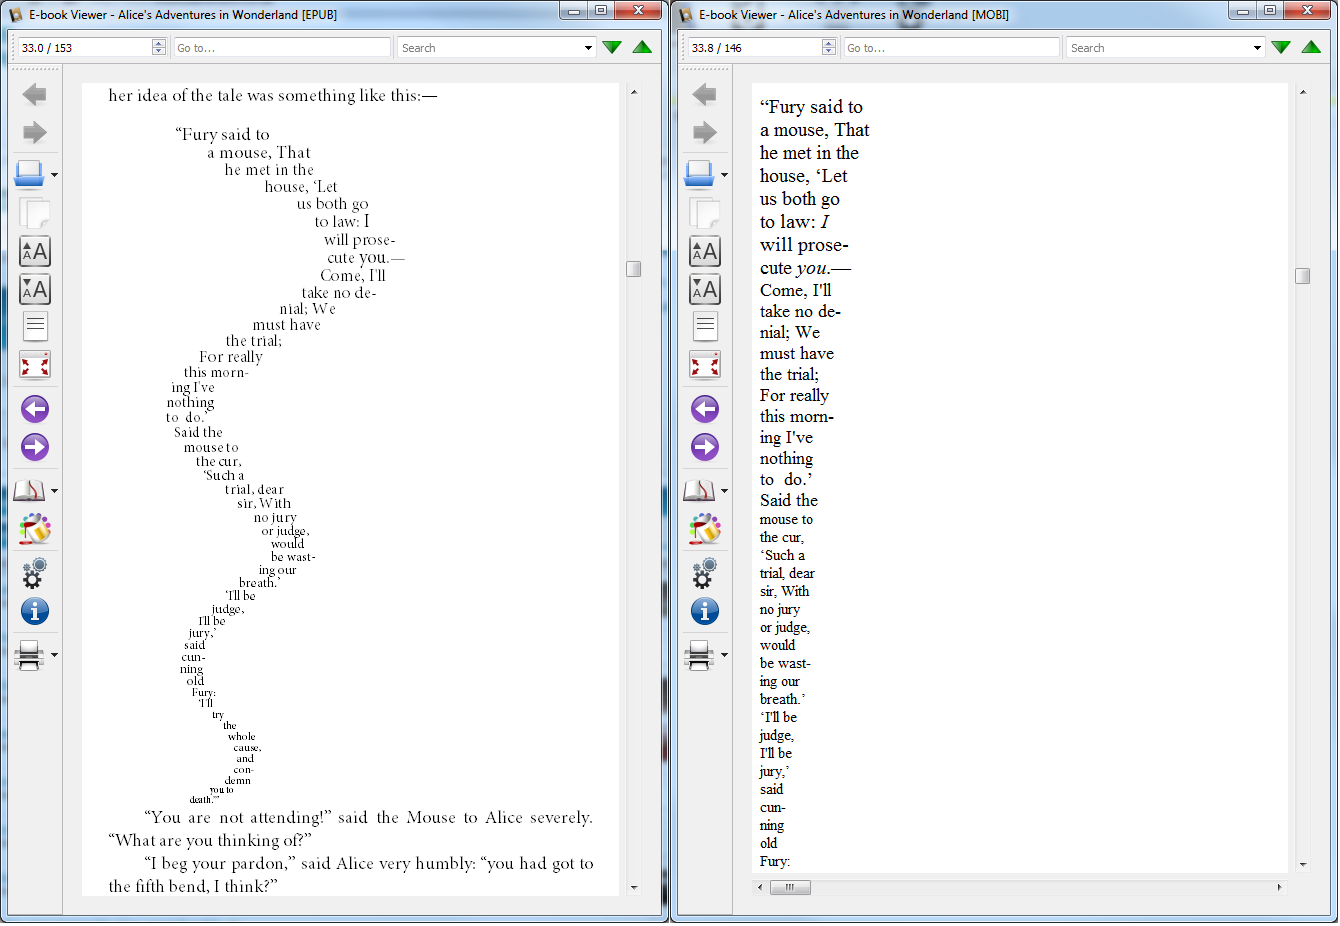
\includegraphics[width=\textwidth]{gfx/alices1}
\caption[Document displayed in Calibre]{On the left is an \epub{} version of Alice in Wonderland, displayed in Calibre (an open source desktop \ebook{} viewer). On the right is the same file, converted to Mobipocket, also displayed in Calibre. Note that in addition to the indentation being lost, the (embedded) font from the \epub{} is no longer present in the Mobipocket file.}
\label{fig:alices1}
\end{figure}

%\marginpar{Mobipocket\ed can't embed fonts... very limited choice of html to use. Reliant on
%rendering engine of device.
%\epub{}\ed can embed fonts, can style with \css{} pretty much arbitrarily, but still needs to be
%retypeset on each viewing and thus relies on the crappy built in rendering engine of the device.}

\epub{} is a little more flexible, in that it supports a more comprehensive range of \xhtml{} and \css{}, and allows for arbitrarily complex styling. \epub{} files are still entirely reliant on the rendering engine of the display device correctly displaying their content, as they have no concrete layout associated with them.

\begin{figure}[tb]
\begin{center}
\vspace{-.3in}
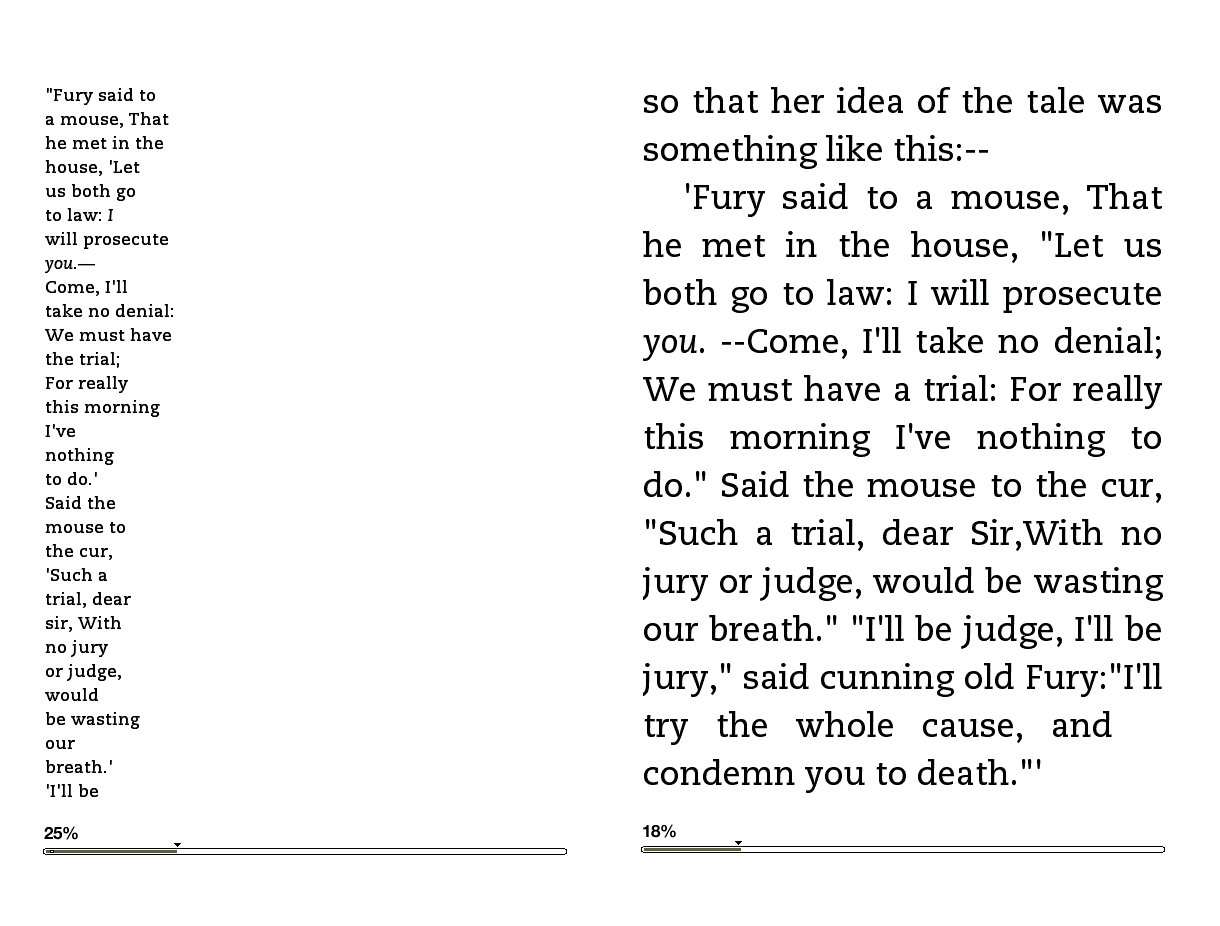
\includegraphics[width=\textwidth]{gfx/alices2}
\end{center}
\vspace{-.3in}
\caption[The same document displayed on the Kindle]{On the left is the Mobipocket version of Alice in Wonderland (from Figure~\ref{fig:alices1}) displayed on the Kindle. Note that the sizing instructions appear to have been ignored. On the right is the free version of Alice in Wonderland from the Kindle store, displayed on the Kindle. Note that no attempt has been made to render the poem in a `tail' shape.}
\label{fig:alices2}
\end{figure}

\section{``Good'' typesetting}
\label{sec:goodtypesetting}

\begin{figure}
    \centering
    \fbox{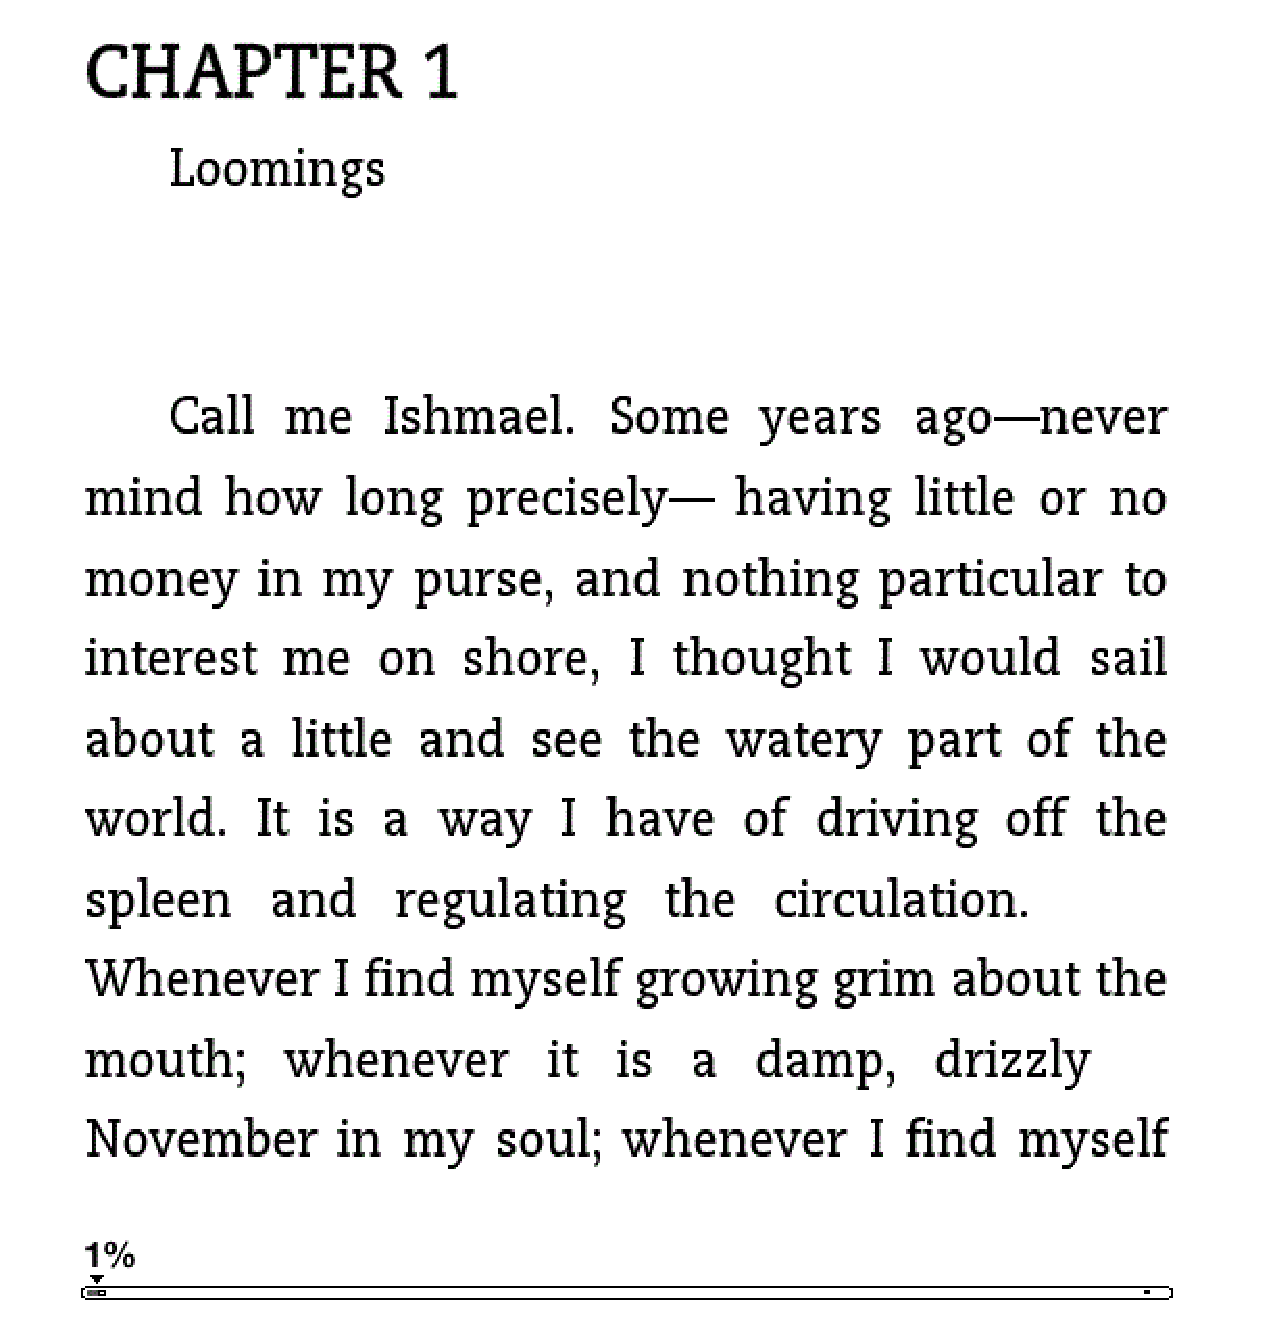
\includegraphics[width=\textwidth
]{gfx/screen_shot-42583}}
    \caption{The Kindle Keyboard appears to primarily use justified text, falling back to ragged-right when inter-word spacing would become too large.}
    \label{fig:crapkindle}
\end{figure}

\subsection{Hyphenation and Line-Breaking}
\Ebook{} readers typically use a `greedy' algorithm to lay out their text\ed that is, they place as many words as will fit onto the current line without exceeding it, then start a new line and continue. Although this algorithm is optimal in that it will always fit text onto the fewest possible lines, it often causes consecutive lines to have wildly varying lengths, accentuating either the `ragged-right' effect of the text, or, in the case of justified text, the inter-word spacing. In general, \ebook{} readers will only hyphenate in extreme cases\ed indeed the Kindle Keyboard seems not to do so at all, to the detriment of its typography (see Figure~\ref{fig:crapkindle}).

Donald E. Knuth and Michael F. Plass~\cite{Knuth1981} developed a more advanced line-breaking algorithm (now used by \TeX{}) which attempts to minimise large discrepancies between consecutive lines by considering each paragraph as a whole. \TeX{} also uses the hyphenation algorithm designed by Franklin Liang~\cite{Liang1983} (another of Knuth's grad students) which has been ported to many other applications.

Knuth and Plass's line breaking algorithm, in conjunction with Liang's hyphenation algorithm, breaks paragraphs into lines of text to fit a page, resulting in what can be considered an aesthetically optimal configuration. \TeX 's default behaviour is then to alter the spacing between words in order to justify the line to fit the measure of the page.

\begin{figure}
 \fbox{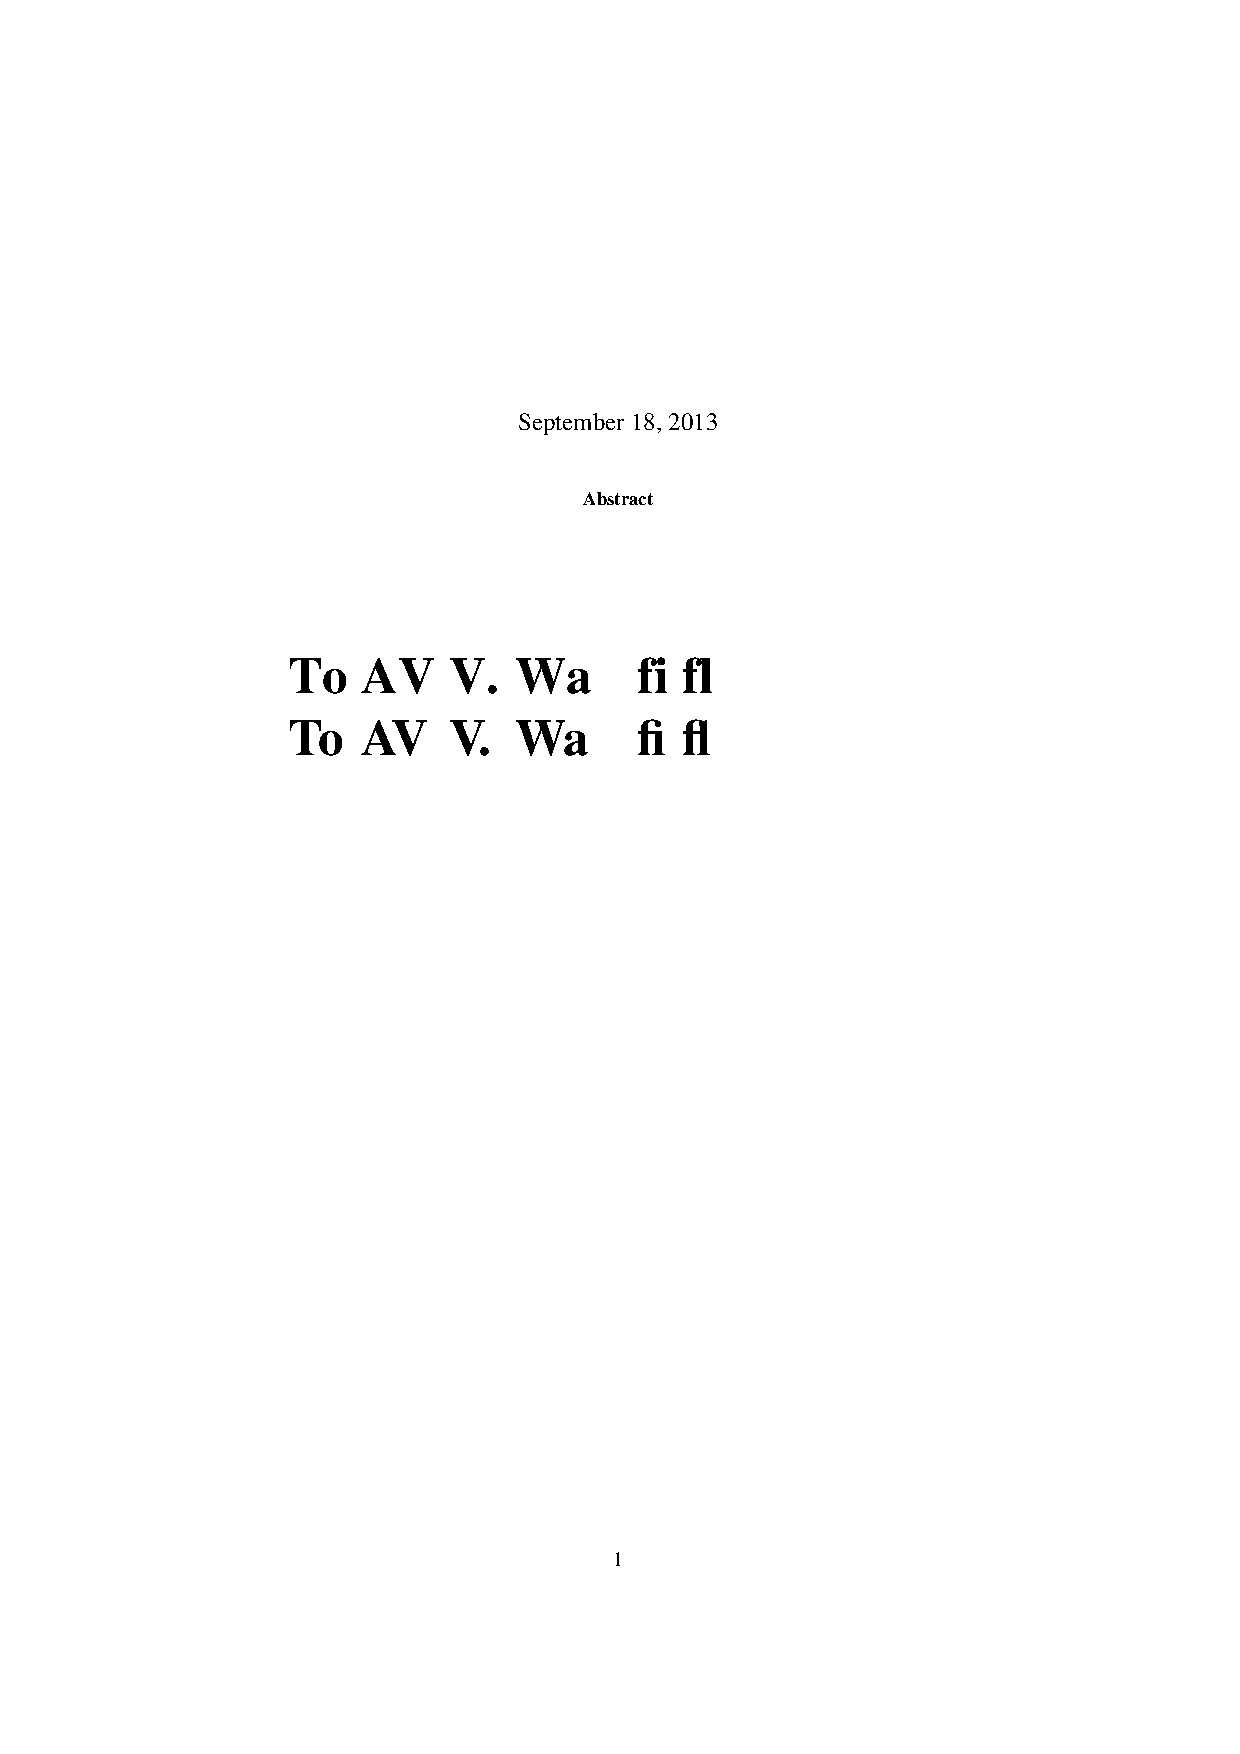
\includegraphics[trim=1.8in 6.54in 3.4in 4.25in, clip=true, width=\textwidth]{gfx/kerningetc}}
 \caption{Examples of various letter-pairs and their kerned (left) or ligature (right) equivalents, as typeset by pdf\LaTeX{}.}
 \label{fig:kern-lig}
\end{figure}

\subsection{Further Typographical Techniques}
Other techniques employed during hand-type\-set\-t\-ing and high-qua\-l\-ity electronic typesetting include the use of kerning and ligatures. Kerning involves altering the spacing between certain glyph pairs in order to produce more consistent letter spacing, and ligatures are sin\-gle-glyph replacements for two or more single glyphs which may otherwise have clashing components. Some examples of these are shown in Figure~\ref{fig:kern-lig}.

Kerning requires a table of kern-pairs, specific to each font; values from this table must then be looked up for every pair of adjacent glyphs in the document. Ligatures may or may not need to be inserted: if the component characters of the ligature lie over a potential hyphenation point, it cannot be decided whether to replace them with the ligature until it is known whether the hyphenation point needs to be used. \TeX{} handles kerning and insertion of ligatures automatically, but there are still further typographical tweaks that its default typesetting algorithm does not use.

More advanced methods than simply stretching or shrinking the word spacing do exist, however. Robert Bringhurst, in \emph{The Elements of Typographic Style}~\cite{Bringhurst2008}, suggests that in addition to altering word spacing, subtle changes to inter-character spacing and individual glyph widths (in the range of $\pm$ 3\%) can produce more typographically and aesthetically pleasing results.

pdf\LaTeX, used to typeset this thesis, \emph{does} make use of all the aforementioned techniques when performing text justification (unlike plain \TeX{} or \LaTeX{}).
 


\part{Implementation}
\cleardoublepage
\chapter{The Malleable Document}\label{ch:malleable}  % ``Aims \& objectives''?? Booooring

%\redmarginpar{This chapter needs to be rewritten. Will probably get to it once the other research chapters are mostly done}
%The real aim of this project is to produce documents that are adaptable to multiple viewing
%apertures, but do not require total reprocessing to do so.

%Chapter~\ref{ch:intro} goes into considerable detail
%about precisely which elements of a typeset document must be considered
%computation-heavy (and thus should be avoided if possible at view-time).
%This chapter goes some way towards defining exactly which portions of the
%typesetting process can be pre-computed and which cannot. It also analyses where shortcuts
%can be taken, and their effects on the final document.

\marginpar{Much of the research in this chapter was previously published in \cite{Pinkney2011}}

The invention of movable type in China in the 11th Century, and independently in Europe in the 15th Century, led to an enormous increase in the availability of printed material. In its various incarnations, movable type formed an extremely important part of the newspaper industry, from its advent in the 17th century, until digitisation in the mid-1980s. The inherently volatile nature of newspaper layout (caused, for example, by important stories breaking shortly before going to press) coupled with the expense and time-consuming nature of physical typesetting, led to the development of the familiar columnar appearance of the newspaper that is prevalent worldwide.

\section{The use of Galleys in Typesetting}
In a traditional newspaper layout, each page is divided into columns of equal \gls{measure}, that is of equal horizontal width. All text that is to appear in the newspaper is typeset to fit this measure (or integer multiples thereof, for example in the case of headlines) allowing articles to be slotted anywhere into the final layout of the newspaper, simply by breaking the article text between lines where necessary to span across columns or pages. An article never requires retypesetting as long as its content remains unchanged\ed{}an advantage only available when all text is rendered to fit into columns of the same width.


The metal trays used to contain typeset lines of physical type are known as \glspl{galley}. Newspapers use reasonably narrow galleys; paperback books tend to use wider galleys, and hardback books wider still. \marginpar{A very unscientific survey of various items of print within arms' reach suggests that newspapers use approximately $2$'' galleys, paperback books around $4$'', and hardback books around $5$''. This thesis uses a galley width of $4\frac{2}{3}$''}Narrower galleys offer the advantage that less space is wasted if the final line in a paragraph does not span the full width: this is more important in newspaper layout than in most other typesetting situations, since space is at a premium. Wider galleys aid readability, up to a certain point, after which it becomes difficult for the eyes to keep track between lines \cite{Bringhurst2008, Braganza2009, Voorhees2011}.

\begin{framed}
{ \footnotesize \parindent0pt
\textsc{Aside:} Renowned typographer Robert Bringhurst \cite{Bringhurst2008} has the following to say about line length:

\begin{quotation}\noindent
Anything from 45 to 75 characters is widely regarded as a satisfactory length of line for a single-column page set in a serifed text face in a text size. The 66-character line (counting both letters and spaces) is widely regarded as ideal. For multiple-column work, a better average is  40 to 50 characters.
\end{quotation}

Bringhurst goes on to say that line lengths exceeding 75--80 characters make continuous reading difficult, and that at the other end of the spectrum, lines shorter than 38--40 characters are unlikely to be easy to fully justify, and should therefore in most cases be set \gls{raggedright}.
}
\end{framed}

Typesetting text into physical galleys is directly analogous to precomputing many of the `hard' parts of typesetting. In particular, all hyphenation, line breaking, \gls{justification}, \gls{kerning}, \gls{glyph} substitution, and so forth (in fact all horizontal layout) is `compiled out'. No matter the height of the page nor the number of columns, only vertical layout problems remain, such as attempting to avoid widowed and orphaned lines (where the last/first lines of a paragraph appear first/last in a column) and choosing optimal placements of figures and other floating bodies. The problem that remains is similar to that described by Michael F. Plass in his Ph.D. thesis \cite{Plass1981}, and by Donald E. Knuth in Chapter~15 of The \TeX{}book~\cite{Knuth1984}.

\section{Galleys as a Reflow Tool}
\label{sec:singlegalleymetric}
If an electronic version of a primarily text-based document is rendered into the analogue of a galley, the document is then provided with some limited flowability. Specifically, the document can be fitted to any page which at least as wide as the galley, and of arbitrary height. Wider pages may be able to accommodate multiple columns, but unless the page size is chosen carefully, based on the galley's width, there is likely to be noticeable extra horizontal whitespace, particularly if the page width is not close to a multiple of the galley width.

\begin{figure}
 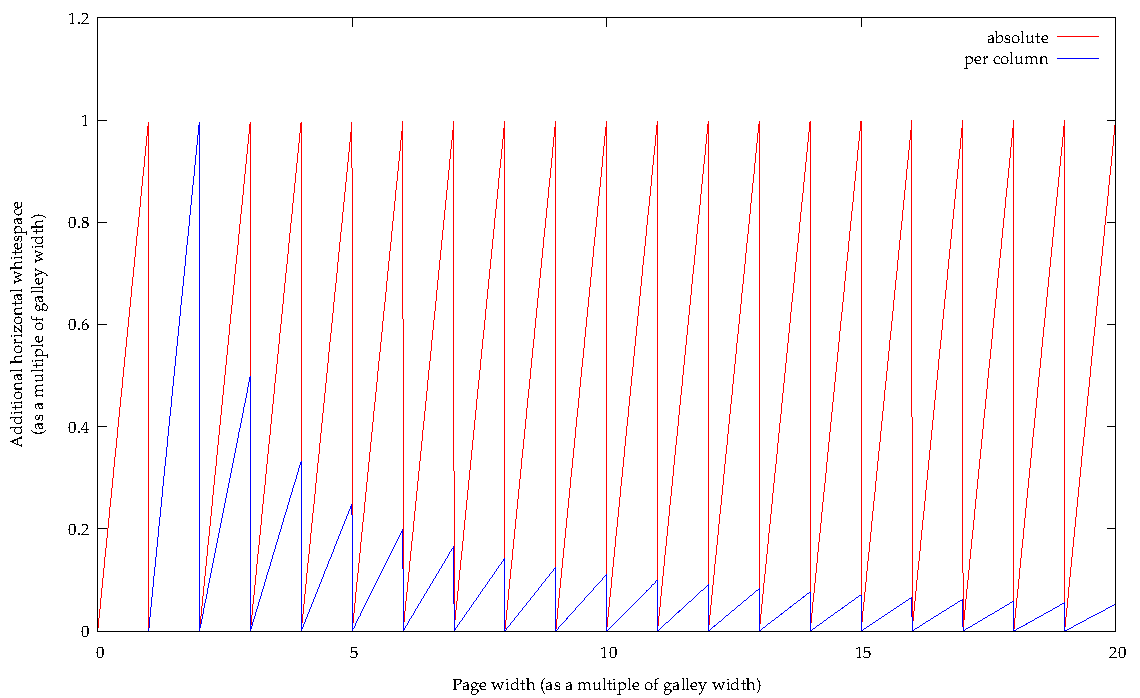
\includegraphics[height=\textwidth,angle=90]{gnuplot/1col}
 \caption[Extra whitespace in a single-galley document]{As more columns fit on a page, the extra whitespace required per column decreases}
 \label{fig:sawtooth}
\end{figure}


Figure~\ref{fig:sawtooth} shows how the extra horizontal whitespace on a page varies with page width. The peaks occur just before the point where an extra column can be added, and the amount of extra whitespace that is required drops to a minimum. The blue line shows the extra whitespace divided by the number of columns that fit on the page, which gives a more useful metric to work with: if we physically divide the extra whitespace and insert it between the columns to increase their spacing (as opposed to leaving it on the right- or left-hand margins) then the wider the page, the less detriment is caused by the extra fraction of galley width.

\section{Multiple Galley Renderings}
\label{sec:multigalleymetric}
The problem of extra whitespace can be overcome in several ways. Firstly, and most simply, the scaling of the galley can be altered, effectively simulating a change in the point size of the font. This is an obvious side-effect and is probably undesirable, unless a change in point size has explicitly been requested, and especially if the size change is particularly noticeable.

A second way in which columns can be better fitted to the page width is to typeset the source document into a range of galleys of varying \gls{measure}. When the document is to be rendered at view-time, the most appropriate measure (according to some metric) can be chosen to be displayed. One very simple metric is to choose whichever galley rendering would result in the least extra added whitespace. By overlaying the Figure \mbox{\ref{fig:sawtooth}-like} graphs for each galley, we are able to obtain a graph like Figure~\ref{fig:overlay}, which features all available galleys. If we use our simple metric of minimum whitespace, we can simply choose whichever galley requires the smallest amount of extra whitespace for a given page width.

\begin{figure}
 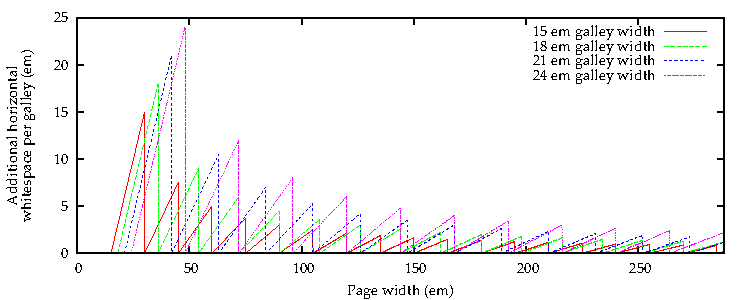
\includegraphics[height=\textwidth,angle=90]{gnuplot/overlay}
 \caption[Extra whitespace in a multi-galley document]{Overlaying the sawtooth graphs for several galleys of differing widths allows us to easily choose the galley that minimises extra added whitespace}
 \label{fig:overlay}
\end{figure}

\section{A Simple Implementation}
At an early stage, it was decided that the simplest available method for a first implementation of the layout algorithm described above was to use some existing tools from the University of Nottingham Document Engineering Laboratory: in particular the \gls{cog} model \cite{Bagley2003} for creating and managing modularised \gls{pdf} documents. This was chosen specifically to avoid the need to write a typesetter or layout engine from scratch; typesetting is performed by the \troff{} suite, and layout by Adobe Acrobat.  % though there is no reason why this algorithm could not be implemented with any other system capable of tightly specifying page imaging operations. Indeed, for this to be implemented in any non-prototypal form, \ie{} to be used on any portable device, it is likely that a specific, new rendering engine will need to be written for each device (or class of device).

\subsection{The \textsc{cog} Model}
%summary of cogs, what I've changed, ie line-level rather than default paragraph level. Put in tree to retain par details
The \gls{cog} model was developed to enable the reuse of semantic components within \pdf{} documents, by breaking the traditional graphically-monolithic \pdf{} page into a series of distinct, encapsulated graphical blocks, termed \glspl{cog}. Initial work on what later became the \gls{cog} model was conducted in the mid 1990s~\cite{Smith1995}, and further developed throughout the 2000s~\cite{Bagley2003,Bagley2004a,Bagley2005,Macdonald2005,Bagley2006,Bagley2007}. The \gls{cog} model, as described in the previous citations, does not account for any relationship between individual \glspl{cog}\,---\,it was simply designed as a method with which document components could be easily reused, reordered, or extracted. The \glspl{cog} generated are largely at the granularity of a paragraph, and still have no compunction to be imaged onto the page in any particular order (for example in reading order).

In order to implement a galley-based design, it is necessary to change the granularity of the \glspl{cog}, such that each line of text is represented by a separate \gls{cog}. However, it is also important that the semantic structure of the document is explicitly stored. This is principally so that the reading order of the \glspl{cog} is maintained, and also so that the reader software can identify paragraphs, headings, and so on, in order to enable them to be laid out correctly at view-time.

The \gls{cog} model takes advantage of the fact that the \pdf{} specification \cite{Adobe2001} allows page content to be described by an array of streams of imaging operators, rather than the more commonly encountered single, monolithic stream. Unfortunately, this array can only be one-di\-men\-sional, meaning that whilst it can enforce reading order, it cannot be used, say, to group lines into paragraphs, or paragraphs into sections.

Since the \pdf{} specification allows essentially arbitrary insertion of data structures into a document, \marginpar{According to the specification, \pdf{} readers that encounter unknown data within a \pdf{} file that they do not recognise should simply ignore it} this flexibility was used to embed a simple tree structure representing the paragraphs, in parallel to the \glspl{cog} themselves. An example of a simple document structure tree is shown in Figure~\ref{fig:tree}. At the level of its leaves, this tree simply contains pointers to the \glspl{cog} which make up the content of the document. In the simplest case, where the document contains only one rendering (and thus the pa\-ra\-graph-level items have only one child) the \glspl{cog} pointed at by the leaves can simply be rendered in order, adding vertical space as appropriate.

\begin{figure}
 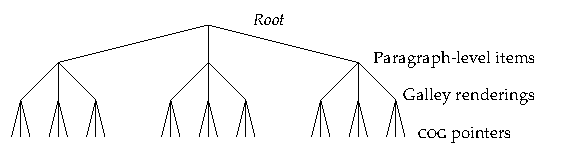
\includegraphics[width=\textwidth]{gfx/tree}
 \caption[A simple document structure tree]{A simple document structure tree. The first level below the root represents all paragraph-level items: headings, paragraphs, figures etc. These items have one child for each galley rendering of the document. These in turn have one child for each \gls{cog} comprising their content\ed{}in the case of a paragraph or heading its lines; in the case of a figure, the figure itself and any associated caption.}
 \label{fig:tree}
\end{figure}

\subsection{The Source Document}\label{sec:srcdoc}
Since the majority of available tools for producing \gls{cog}ged \glspl{pdf} rely on the typesetting package \ditroff{}~\cite{Kernighan1982}, it was decided to use this as the basis for the source document. \Ditroff{} is particularly amenable to many of the features required here\ed{}it is quite happy to have its page length set to large values\ed{}one sample document used a page length of 2000 inches (approximately 50 metres) with no complaints from \ditroff{}. The line length was set to a small value (approximately two inches) in order to produce a narrow column of text. Following this, the actual document content was inserted several times, and the line length increased after each iteration, producing one document effectively containing multiple galley-width renderings of the same content. An example of a source document is shown in Listings \ref{lst:troffsourcedoc1}~and~\ref{lst:troffsourcedoc2}.

\begin{lstlisting}[label=lst:troffsourcedoc1,captionpos=b,float,caption={[A sample troff source document, part 1]A sample troff source document. The actual document text is in a file named {\tt contents.inc} , and is imported multiple times with the {\tt .so} macro. After each import, the current line length is changed (using, for example, {\tt .nr LL 1.5i} to set Line Length register to 1.5 inches). The {\tt \textbackslash X} commands are used to pass arbitrary data through the typesetter, and into the resultant ditroff intermediate code for later use. In this case, it is used to pass the column width (hence ``cWidth'') in points, so that this data can later be embedded within the final \pdf{} file.}]
.nr HM 0.5i
.nr FM 0.5i
.ds CH 
.\" Overwrites the Centre Header (suppresses page number)
.pl 2000i
.\" Make the page quite long to avoid troff doing any pagination
.nr PO 0
.\" set Page Offset (ie left margin) to zero
.ps 11
.vs 13
.nr PS 11
.nr VS 13
.\" Set point size to 11 and vertical spacing (leading) to 13
.\" Below, alter value of LL (line length) and include document
.\" content with the .so macro
.nr LL 1i
\X'cWidth:72'
.\" Line Length (ie galley width)
.so contents.inc
.nr LL 1.5i
\X'cWidth:108'
.so contents.inc
.nr LL 2i
\X'cWidth:144'
.so contents.inc
.nr LL 2.5i
\X'cWidth:180'
.so contents.inc
.nr LL 3i
\X'cWidth:216'
.so contents.inc
.nr LL 3.5i
\X'cWidth:252'
.so contents.inc
.nr LL 4i
\X'cWidth:288'
.so contents.inc
\end{lstlisting}


\begin{lstlisting}[label=lst:troffsourcedoc2,captionpos=b,float,caption={[A sample troff source document, part 2]A three-paragraph excerpt from a sample {\tt contents.inc} file, as described in Listing~\ref{lst:troffsourcedoc1}. Each paragraph is preceded by a call of the {\tt.PP} macro, which signifies the start of a new paragraph.}]
.PP
Lorem ipsum dolor sit amet, consectetur adipiscing elit. Cras vel
enim vitae mauris vestibulum egestas. Suspendisse potenti.
Pellentesque leo nunc, lobortis vitae gravida vel, congue at
nulla. Praesent a placerat mauris. Praesent sed erat ac dui
tincidunt consectetur vel nec leo. In velit odio, congue non
eleifend at, accumsan eu diam. Suspendisse dignissim, quam quis
euismod laoreet, est leo euismod lectus, sed consequat leo nunc
in ante. Duis risus tellus, suscipit ut fermentum et, ornare non
lorem. Morbi nibh elit, dignissim ullamcorper posuere at, lacinia
condimentum odio. Fusce vitae metus mi. Pellentesque scelerisque
fermentum magna a dictum. Mauris ut ante mauris, ac viverra
felis. Praesent ut elit ut purus malesuada suscipit. Fusce mollis
eros ac lectus suscipit gravida. Pellentesque vel nisl nec eros
convallis luctus nec eu quam. Aliquam tincidunt ultrices blandit.
.PP
Vestibulum lorem felis, consectetur ornare vehicula ac, cursus
tincidunt nisl. Aliquam in enim nisi, quis hendrerit est. Nullam
pretium congue sapien ac tincidunt. Suspendisse suscipit felis
eget nibh luctus sit amet imperdiet ligula venenatis. Vestibulum
eu dui nulla. Vivamus interdum ullamcorper sapien eget dapibus.
Proin sed dictum arcu. Curabitur velit justo, fringilla non
sodales laoreet, dignissim nec nulla. Praesent convallis ipsum
quis dolor ultricies non sodales dui viverra. Phasellus nec nisi
at nisi bibendum aliquam vitae et arcu. Donec feugiat dolor ut
felis dapibus eget auctor enim mattis.
.PP
Curabitur eget eros neque, in pulvinar massa. Suspendisse ac
massa quis justo fringilla consectetur. Vivamus lacinia tincidunt
purus, sit amet ullamcorper neque imperdiet quis. Nulla at lectus
turpis, in semper augue. Donec eu rhoncus turpis. Maecenas lectus
lacus, porta et dictum eget, eleifend a nibh. Vestibulum pulvinar
pellentesque lectus, et tincidunt eros consequat sed. Duis risus
lorem, placerat et molestie ut, porta a mi. Fusce eu elit enim,
id consequat nibh. Cras elementum, odio a tristique rutrum, nibh
neque sodales lorem, eu feugiat ipsum leo a nunc. Quisque enim
felis, luctus dapibus iaculis ac, tempor vitae lacus. Nunc eu mi
quis lacus scelerisque tincidunt. Sed sed nulla dui. Suspendisse
porta imperdiet tortor vel ultricies. Donec sit amet ligula
velit. Nulla tempor, risus sit amet congue aliquam, est nulla
tincidunt lectus, scelerisque cursus lacus diam vel metus. Donec
eu elit dolor. Nullam id libero ac metus ornare iaculis id ut
lorem. Quisque iaculis justo nec nibh interdum vuPPutate.
\end{lstlisting}

\subsection{pdfdit}
Having created the source document, it was processed with \ditroff{} to generate the intermediate code used to feed each typesetter post-pro\-cessor. This output is very expressive, and, unlike \TeX's equivalent DVI, contains enough information that post-processors are easily able to locate the start and end of lines and paragraphs within the document. This meant that only minimal changes were needed to the \emph{pdfdit} package described in \cite{Bagley2003} to implement the design.

The first change necessary was to decrease the granularity of the output \gls{cog}s, producing them at the line level, rather than at the paragraph level. Secondly, some method of generating the requisite tree representing the document structure was required. This was solved by simply using the point at which the original version of pdfdit would have started a new paragraph-level \gls{cog}, and, instead, starting a new paragraph-level block entry in the document structure tree. Each subsequent line-level \gls{cog} produced can then be added as a child of this block.

Once the entire output file has been parsed, the tree representations of the various width galleys are amalgamated per-paragraph, as indicated in Figure~\ref{fig:tree}, and finally the \pdf{} file is serialised, replete with \gls{cog}s and document structure tree. Various key excerpts from a malleable \pdf{} file's internal structure is shown in Listings \ref{lst:pdfstart}, \ref{lst:pdfpartree}, \ref{lst:pdfcog}, and~\ref{lst:pdfpages}.

\begin{lstlisting}[label=lst:pdfstart,captionpos=b,language=postscript,float,caption={[Excerpt from a malleable document \pdf{}]An excerpt from a the start of a malleable document \pdf{} file. A reference to the \texttt{/ParagraphData} object (shown in Listing~\ref{lst:pdfpartree}) has been added to the \pdf{}'s \texttt{/Catalog} object. The \texttt{/Pages} object is also shown\ed{}note that there is only ever one page in a malleable \pdf{}.}]
%PDF-1.4
1 0 obj
<<
 /Type /Catalog
 /Pages 2 0 R
 /CogData 7472 0 R
 /ParagraphData 7473 0 R
>>
endobj
2 0 obj
<<
 /Type /Pages
 /Kids [7471 0 R  ]
 /Count 1
>>
endobj
\end{lstlisting}


\begin{lstlisting}[label=lst:pdfpartree,captionpos=b,language=postscript,float,caption={[Excerpt from a document structure tree]An excerpt from a document structure tree in a malleable document \pdf{} file. The tree structure described in Figure~\ref{fig:tree} can be observed in the \texttt{/Paragraphs} array, with the exception that the first element is an array containing the widths of each included galley rendering.}]
7473 0 obj
<<
 /Type /Multi-Width
 /Paragraphs
 [
    [72 108 144 180 216 252 288] % Width of each set of paragraphs, in points (ie 72*inch)
    [ % Paragraph 1
        [4 0 R 6 0 R 8 0 R 10 0 R 12 0 R 14 0 R 16 0 R 18 0 R 20 0 R 22 0 R 24 0 R 26 0 R 28 0 R 30 0 R 32 0 R 34 0 R 36 0 R 38 0 R 40 0 R 42 0 R 44 0 R 46 0 R 48 0 R 50 0 R 52 0 R 54 0 R 56 0 R 58 0 R 60 0 R 62 0 R 64 0 R 66 0 R 68 0 R 70 0 R 72 0 R 74 0 R 76 0 R 78 0 R 80 0 R 82 0 R 84 0 R 86 0 R 88 0 R 90 0 R 92 0 R 94 0 R 96 0 R 98 0 R 100 0 R 102 0 R 104 0 R 106 0 R 108 0 R 110 0 R 112 0 R 114 0 R 116 0 R 118 0 R 120 0 R 122 0 R 124 0 R 126 0 R 128 0 R 130 0 R 132 0 R 134 0 R]
        [2303 0 R 2305 0 R 2307 0 R 2309 0 R 2311 0 R 2313 0 R 2315 0 R 2317 0 R 2319 0 R 2321 0 R 2323 0 R 2325 0 R 2327 0 R 2329 0 R 2331 0 R 2333 0 R 2335 0 R 2337 0 R 2339 0 R 2341 0 R 2343 0 R 2345 0 R 2347 0 R 2349 0 R 2351 0 R 2353 0 R 2355 0 R 2357 0 R 2359 0 R 2361 0 R 2363 0 R 2365 0 R 2367 0 R 2369 0 R 2371 0 R 2373 0 R 2375 0 R 2377 0 R 2379 0 R 2381 0 R 2383 0 R]
        [3755 0 R 3757 0 R 3759 0 R 3761 0 R 3763 0 R 3765 0 R 3767 0 R 3769 0 R 3771 0 R 3773 0 R 3775 0 R 3777 0 R 3779 0 R 3781 0 R 3783 0 R 3785 0 R 3787 0 R 3789 0 R 3791 0 R 3793 0 R 3795 0 R 3797 0 R 3799 0 R 3801 0 R 3803 0 R 3805 0 R 3807 0 R 3809 0 R 3811 0 R 3813 0 R]
        [4821 0 R 4823 0 R 4825 0 R 4827 0 R 4829 0 R 4831 0 R 4833 0 R 4835 0 R 4837 0 R 4839 0 R 4841 0 R 4843 0 R 4845 0 R 4847 0 R 4849 0 R 4851 0 R 4853 0 R 4855 0 R 4857 0 R 4859 0 R 4861 0 R 4863 0 R 4865 0 R 4867 0 R]
        [5661 0 R 5663 0 R 5665 0 R 5667 0 R 5669 0 R 5671 0 R 5673 0 R 5675 0 R 5677 0 R 5679 0 R 5681 0 R 5683 0 R 5685 0 R 5687 0 R 5689 0 R 5691 0 R 5693 0 R 5695 0 R 5697 0 R 5699 0 R]
        [6355 0 R 6357 0 R 6359 0 R 6361 0 R 6363 0 R 6365 0 R 6367 0 R 6369 0 R 6371 0 R 6373 0 R 6375 0 R 6377 0 R 6379 0 R 6381 0 R 6383 0 R 6385 0 R]
        [6951 0 R 6953 0 R 6955 0 R 6957 0 R 6959 0 R 6961 0 R 6963 0 R 6965 0 R 6967 0 R 6969 0 R 6971 0 R 6973 0 R 6975 0 R 6977 0 R 6979 0 R]
    ] % Note: "<x> <y> R" is a pointer to the object defined with "<x> <y> obj" -- these all point to COG spacer objects
    [ % Paragraph 2
        [136 0 R 138 0 R 140 0 R 142 0 R 144 0 R 146 0 R 148 0 R 150 0 R 152 0 R 154 0 R 156 0 R 158 0 R 160 0 R
%%% truncated %%%
\end{lstlisting}

\begin{lstlisting}[label=lst:pdfcog,captionpos=b,language=postscript,float,caption={[A \textsc{cog} and its associated spacer object]A \gls{cog} (object 2303) and its associated spacer (object 2304) from a malleable \pdf{}. The \gls{cog} object is never modified. To reposition the \gls{cog} on the page, the spacer object is deleted and replaced with a new one that has the required \texttt{/X} and \texttt{/Y} values set.}]
2303 0 obj
    <<
        /Type /XObject
        /Subtype /Form
        /Name /Cog8f692dee-5919-11e0-90bd-9eb109602c3e
        /FormType 1
        /BBox [0.000000 0.000000 82.933000 9.889000  ]
        /Baseline 2.387000
        /Indent 25.000000
        /Length 219
        /Resources <<
            /Font <<
                /R 3 0 R
            >>
            /ProcSet [/PDF /Text  ]
        >>
    >>
    stream
        q
        0.125000 0 0 0.125000 0 0 cm
        BT
        /R 1 Tf
        88.000000 0 0 88.000000 0.000000 19.096000 Tm (Lorem ) Tj
        88.000000 0 0 88.000000 448.000000 19.096000 Tm (i) Tj
        88.000000 0 0 88.000000 473.000000 19.096000 Tm (psum ) Tj
        ET
        Q
    endstream
endobj

2304 0 obj
    <<
        /Type /CogReference
        /Height 9.889000
        /Length 83
        /ptrTo /Cog8f692dee-5919-11e0-90bd-9eb109602c3e
        /X 25.000000
        /Width 82.933000
        /Y -14118.497000
    >>
    stream
        q 1 0 0 1 25.000000 -14118.497000 cm /Cog8f692dee-5919-11e0-90bd-9eb109602c3e Do Q 
    endstream
endobj
\end{lstlisting}


\begin{lstlisting}[label=lst:pdfpages,captionpos=b,language=postscript,float,caption={[Contents of a \pdf{} \texttt{Page} object]An excerpt from a malleable \pdf{} file showing that the \texttt{/Contents} of a \texttt{/Page} can be an array of content streams rather than one stream. In this case, each of the objects being pointed to are \gls{cog} spacers, as shown in Listing~\ref{lst:pdfcog}. Consequently, when a spacer object is deleted and a new one created (to reposition a \gls{cog} on the page) the \texttt{/Contents} array must be modified to reflect this.}]
7471 0 obj
<<
 /Type /Page
 /Subtype /Cogified
 /MediaBox [0 0 595 841]
 /Contents [5 0 R 7 0 R 9 0 R 11 0 R 13 0 R 15 0 R 17 0 R 19 0 R 21 0 R 23 0 R 25 0 R 27 0 R 29 0 R 31 0 R 33 0 R 35 0 R 37 0 R 39 0 R 41 0 R 43 0 R 45 0 R 47 0 R 49 0 R 51 0 R 53 0 R 55 0 R 57 0 R 59 0 R 61 0 R 63 0 R 65 0 R 67 0 R 69 0 R 71 0 R 73 0 R 75 0 R 77 0 R 79 0 R 81 0 R 83 0 R 85 0 R 87 0 R 89 0 R 91 0 R 93 0 R 95 0 R 97 0 R 99 0 R 101 0 R 103 0 R 105 0 R 107 0 R 109 0 R 111 0 R 113 0 R 115 0 R 117 0 R 119 0 R 121 0 R 123 0 R 125 0 R 127 0 R
%%% truncated %%%
\end{lstlisting}

\newpage %sozboz
\subsection{Acrobat Plugin}\label{sec:acroplugin}
\begin{figure}
 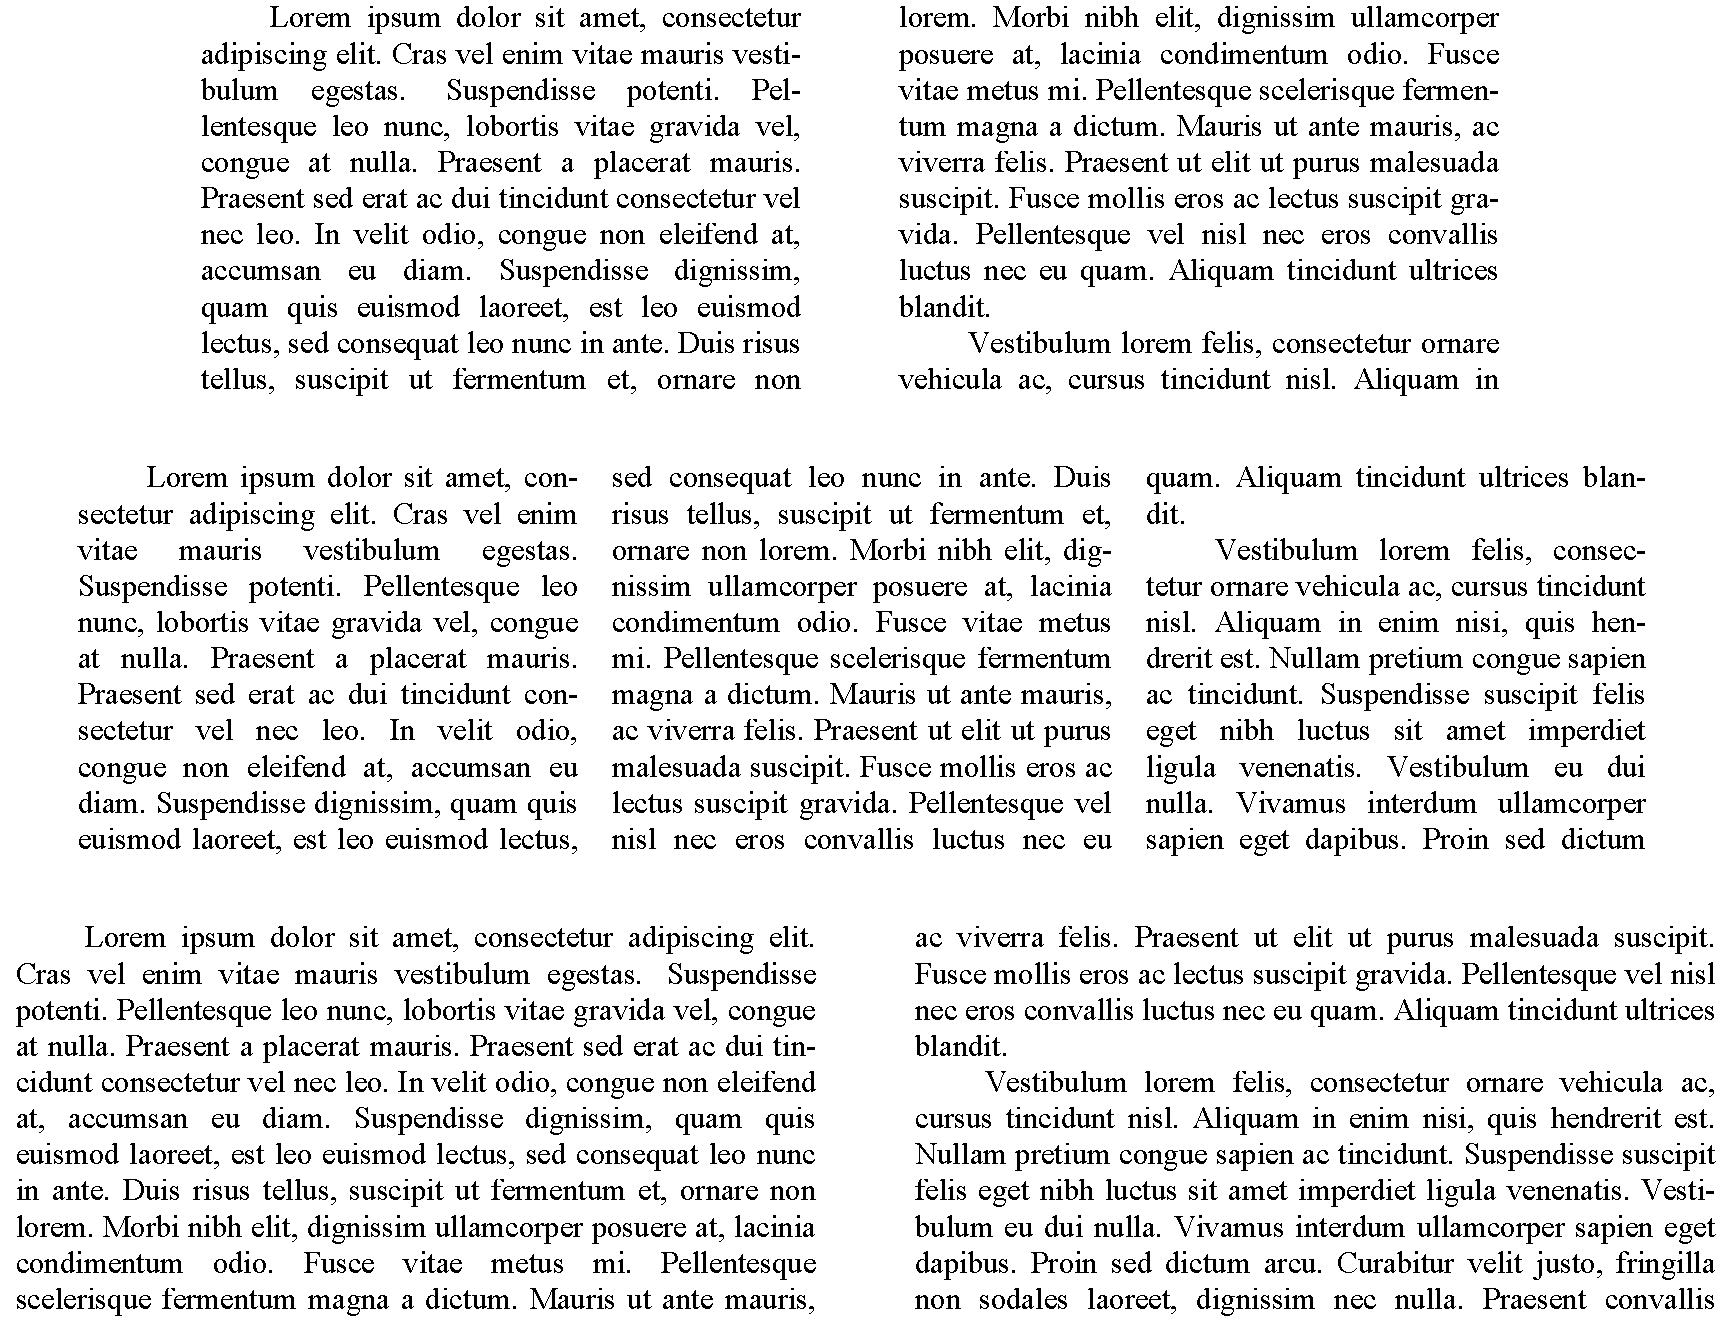
\includegraphics[width=\textwidth]{gfx/renderings}
 \caption[Sample renderings from the Acrobat plugin]{Three sample renderings from the Acrobat plugin, with page widths of 42, 48, and 54~em.}
 \label{fig:renderings}
\end{figure}

The decision to use Acrobat as an \ebook{} `emulator' stemmed once again from the available existing \gls{cog}-based tools (see Section \ref{sec:srcdoc}), as well as the extensive API and developer support available for Acrobat.

Since, by the point the document is to be displayed in Acrobat, most of the computationally expensive typesetting has already been carried out, the algorithm used to lay out the lines of the galleys can be very simple. The plugin chooses the most appropriate galley width to lay out, based on the current page width, and according to some measure of aesthetics, and then simply lays the document out line by line, with appropriate vertical spacing, until no more lines will fit in the current column. Any subsequent columns which will fit on the same page are then laid out in the same manner.

For convenience of testing, the plugin also automatically resizes the page to that of the window of Acrobat, and re-lays out the text on the fly, allowing various combinations of page sizes, zoom levels, and aspect ratios to be trialled.
Some sample renderings from the Acrobat plugin are shown in Figure~\ref{fig:renderings}, and an excerpt of the code used for the layout is shown in Listing~\ref{lst:acrolayout}.

\begin{lstlisting}[language=c++,tabsize=4,basicstyle=\ttfamily\scriptsize\singlespacing,stringstyle=\color{blue},label=lst:acrolayout,captionpos=b,float,caption={[Acrobat plugin's layout algorithm]An excerpt from the C++ Acrobat plugin, showing the implementation of the layout algorithm described in Section~\ref{sec:acroplugin}.}]
int numPars = CosArrayLength(parArray) - 1; // first element is not a paragraph
CosObj widthsArray = CosArrayGet(parArray, 0); // it is the widths array
int numWidths = CosArrayLength(widthsArray);
ASFixed *widths = (ASFixed*)calloc(numWidths, sizeof(ASFixed));
double *badness = (double*)calloc(numWidths, sizeof(double));

int min_badness_index = 0;
int numCols = 0;

// Choose the "best" rendering
for (int i = 0; i < numWidths; i++) {
    widths[i] = CosFixedValue(CosArrayGet(widthsArray,i));
    int nc = pageWidth / (widths[i] + mingutter);
    ASFixed ex_ws = pageWidth % (widths[i] + mingutter);
    
    badness[i] = (ex_ws / 65536.0 + 100) * sqrt((double)nc);
    
    if (nc == 0) badness[i] = 1000 * i;
    
    if (badness[i] <= badness[min_badness_index]) {
        min_badness_index = i;
        numCols = nc;
    }
}

ASFixed colsep = pageWidth / numCols;
ASFixed linesep = 13<<16; // 13pt. (Ideally, infer from data within PDF)
ASFixed parsep = 0;

int curr_x = mediabox.left + (colsep - widths[min_badness_index]) / 2;
int curr_y = mediabox.top - topmargin;

CosObj newContents = CosNewArray(cosDoc, false, 100);

// Create new spacer objects with correct COGs, and insert into newContents
for (int p = 0; p < numPars; p++) {
    CosObj para = CosArrayGet(CosArrayGet(parArray, p + 1), min_badness_index);
    int numLines = CosArrayLength(para);
    for (int l = 0; l < numLines; l++) {
        CosObj baseline = CosDictGet(CosStreamDict(CosArrayGet(para, l)), ASAtomFromString("Baseline"));
        CosObj indent = CosDictGet(CosStreamDict(CosArrayGet(para, l)), ASAtomFromString("Indent"));
        CosObj name = CosDictGet(CosStreamDict(CosArrayGet(para, l)), ASAtomFromString("Name"));
        
        int y_offset = CosFixedValue(baseline);
        int x_offset = CosFixedValue(indent);
        
        if (curr_y < (mediabox.bottom + botmargin)) { //start new column
            curr_y = mediabox.top - topmargin;
            curr_x += colsep;
        }
        
        CCosDoc cDoc(cosDoc);
        CSpacerCreator spacerCreator(cDoc);
        CCosStream newSpacer = spacerCreator.Create(ASAtomGetString(CosNameValue(name)), curr_x + x_offset, curr_y - y_offset);
        
        CosArrayInsert(newContents, CosArrayLength(newContents), newSpacer);
        
        curr_y -= linesep;
    }
    curr_y -= parsep;
}

PDPageAddCosContents(page, newContents);


\end{lstlisting}


\section{Layout Considerations}
\begin{sidewaysfigure}
 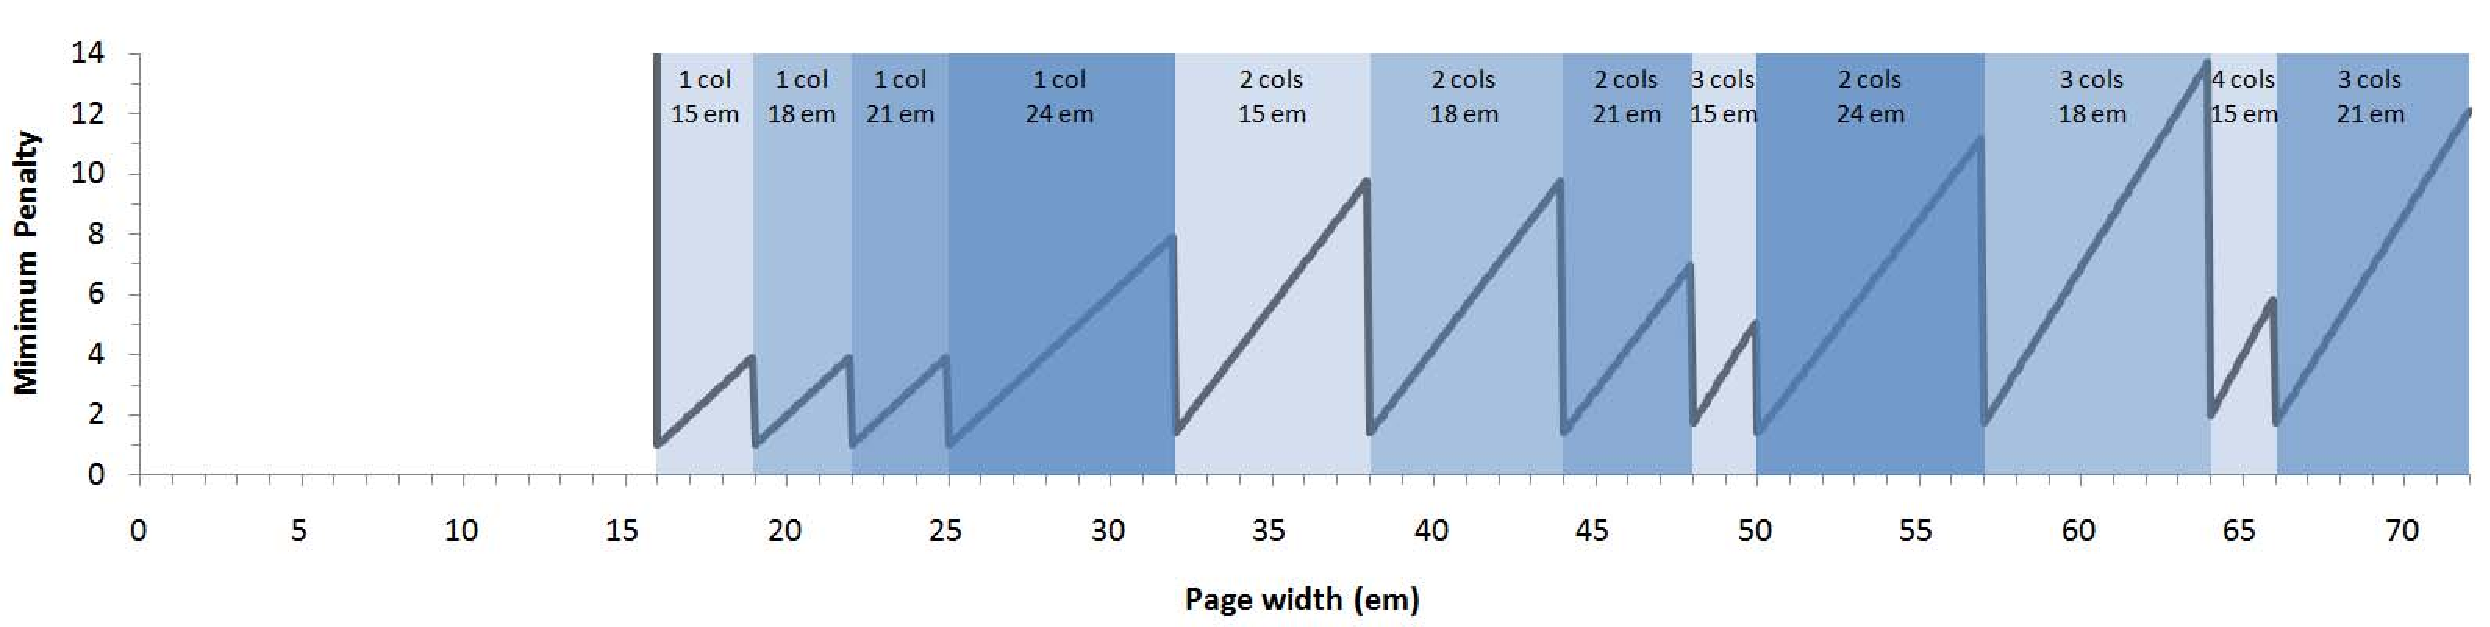
\includegraphics[width=\textwidth]{gfx/graph-em}
 \caption[Graph of minimum penalty values]{Graph showing the minimum penalty value of all galleys in a reflowable document, over a range of page widths. The particular document used contained four galleys; these were rendered at widths of 15, 18, 21 and 24~em, with a minimum gutter width of 1~em. Each vertical band highlights a range of page widths within which only the horizontal spacing of the page is altered. The boundaries between vertical bands represent a switch between galley renderings\ed{}the galley used and number of columns is as annotated on the graph.}
 \label{fig:penaltygraph}
\end{sidewaysfigure}

As discussed in Sections \ref{sec:singlegalleymetric} and~\ref{sec:multigalleymetric}, galleys of text lend themselves to being used in a columnar format, and therefore a method of fitting columns appropriately to the available page width must be devised. A sensible first approach is simply to calculate how many columns of each galley rendering will fit, by adding the galley width to a specified minimum inter-column spacing, and dividing the page width by this. The remainder of this division will then specify the total extra amount of horizontal whitespace required, which can then divided up and inserted between the columns. A simple measure of aesthetic quality here is to apply a linear penalty for any extra whitespace required, as we seek to keep page margins and column gutters to a minimum.

Equations \ref{eqn:numcols} and~\ref{eqn:extraws} below show the formulae used to calculate the number of columns that will fit ($N_\text{cols}$), and the requisite extra whitespace ($S_\text{extra}$). $W_\text{page}$ is the total width of the page, $W_\text{galley}$ is the width of the current galley, and $W_\text{ICS}$ is the minimum required inter-column spacing.
\begin{equation}\label{eqn:numcols}
N_\text{cols}=\left\lfloor\frac{W_\text{page}}{W_\text{galley}+W_\text{ICS}}\right\rfloor
\end{equation}
\begin{equation}\label{eqn:extraws}
S_\text{extra}=W_\text{page}\!\!\mod \left(W_\text{galley}+W_\text{ICS}\right)
\end{equation}

As the page width increases, so must the widths of the inter-column gutters. In accordance with the extra-whitespace penalty, each galley rendering will produce penalties which vary in a sawtooth manner as the width of the page is increased. With a careful choice of galley widths, when these sawtooth penalties are overlaid, and the galley producing the minimum penalty chosen at each page width, a flatter and finer-toothed penalty graph emerges, as shown in Figure~\ref{fig:penaltygraph}.

In addition to penalising extra whitespace, wider columns should, in general, be favoured over narrower ones, i.e.~for a given page width, fewer, wider columns are generally considered preferable to a greater number of narrower columns. By multiplying the existing penalty by a smaller-than-linear function of the number of columns (experiments have been carried out with both logarithms and roots) the penalty may be subtly increased for greater numbers of columns.

The formula for the penalty used in Figure~\ref{fig:penaltygraph} is \begin{equation}P = (C + S_\text{extra})\cdot\sqrt{N_\text{cols}}\end{equation} where $P$ is the penalty, $S_\text{extra}$ is the extra whitespace required to be inserted (as computed in equation~\ref{eqn:extraws}), $N_\text{cols}$ is the number of columns which are required to fill the width of the page (as computed in equation~\ref{eqn:numcols}), and $C$ is a positive constant.

The purpose of the constant is to prevent the penalty from ever evaluating to zero, which would have the effect of disregarding the weighting of the number of columns. Figure~\ref{fig:penaltygraph} uses $C=1$.
%eg what sort of layouts are we constricted to, and are they any good... cite Plass/Bringhurst

\section{Included galley renderings}
\label{sec:inc-renderings}
In order for a document to achieve optimal fit on every device of every conceivable size, we must produce one galley rendering of every conceivable width. Clearly, \marginpar{As one of my colleagues once shouted in exasperation: ``infinity is not an option!''} this is infeasible, both in terms of space and time. For reasons of practicality, we are therefore forced choose some non-infinite subset of galley widths to include within a document.

Some experimentation has suggested that using between three and seven galley renderings, ranging in width between two and five inches (set in twelve point type) provides acceptable coverage on a variety of device sizes. Whether the sampling range within these bounds should be linear, or based on some other function, is still open for debate, and requires further experimentation.




\section{Efficiency}
%theoretically, how does it compare? Shove in lots of speculative Big Oh notation and try to sound authoritative. Or look at the algorithms used and actually be authoritative :)

It can easily be observed that the view-time complexity of the layout algorithm described in this chapter is linear.

At view-time, it must be decided which galley rendering to display: this is a trivial operation that requires one calculation per galley rendering. Assuming that there will never be more than ten galley renderings within one document (this seems reasonable given the discussion in Section~\ref{sec:inc-renderings}) the time taken to choose the best-fitting galley will always be dominated by the time taken to perform the layout itself.

After the rendering to display has been chosen, all that is left is to traverse the document structure tree, laying out each line of text sequentially. If there are $n$ lines of text in the document, this takes at most $k\cdot{}n$ operations, where $k$ is some constant pertaining to operations required to lay out one line of text, and therefore the view-time complexity is $O(n)$.

A first-fit (or greedy) layout algorithm, as used by most current \ebook{} hardware and web browsers, also runs in $O(n)$ (proportional to the number of possible breakpoints, $n$) though its layout will almost certainly be substandard in comparison to any high-quality pre-rendered layout, as used by the system described in this chapter. Conversely, to compute this high-quality layout on the fly, (using, for example, the Knuth-Plass line breaking algorithm \cite{Knuth1981,Knuth1999}, or something even more complex) can take upwards of $O(n^2)$~\cite{Eppstein1992,Hirschberg1987,Hurst2009,Pinkney2013}.

\section{Summary}
The drawbacks of this system are that the filesize is necessarily increased (since data for multiple layouts must be included), and that the galley rendering that is displayed may not fit the available page width as snugly as an algorithm that has been run on the fly (and is therefore specifically tailored to the dimensions of the page). In spite of this, this galley-based system produces pleasing-looking, well formatted documents.

The implementation of this algorithm within Adobe Acrobat is somewhat clunky (and certainly impractical to deploy on a real \ebook{} platform) but it demonstrates that the concept of pre-rendering several variants is a viable means to producing well-typeset flowable layouts. The one notable omission from this chapter is support for floating blocks (such as figures)\ed only non-floating blocks are supported. In the next chapter, both of these issues are addressed.


\cleardoublepage
\chapter{Floatable Blocks}\label{ch:floats}

\marginpar{The research in\\ this chapter was previously described in \cite{Pinkney2013}}

% Required implementation:
% \begin{itemize}
%     \item extension of chapter 2 code to support floats
%     \item tradeoffs between Plass\cite{Plass1981} pagination and `dumb' pagination. Should floats be
%     `floatable'?
%     \begin{itemize}
%         \item how floatable?
%         \item how much effort do we put in before it stops being worth it?
%     \end{itemize}
%     \item Floats across multiple columns?
%     \begin{itemize}
%         \item simple multiples of galley width/line height
%     \end{itemize}
%     \item Bringhurst's suggestion\cite{Bringhurst2008} of making blocks take up multiples of the
%     leading to always keep text in phase (could even factor this into chapter 2 implementation)
% 
% \end{itemize}

The system described in Chapter~\ref{ch:malleable} supports only simple documents that are composed solely from text. Many (perhaps most) real-world documents contain figures, diagrams, illustrations, tables etc., and so consideration must be given towards how these should be handled.

This chapter extends the work of the previous chapter to allow floatable graphical blocks, whose absolute position within a document's text may vary, depending upon the layout.

%\section{Implementation}

The implementation of the system described in the previous chapter is deeply rooted within \gls{pdf}, and requires a custom-written plugin for Adobe Acrobat (see Section~\ref{sec:acroplugin}) to view the documents. Consequently, it is difficult to test that particular implementation on any device that is not running Microsoft Windows and does not have a fully licensed version of Adobe Acrobat, which effectively rules out any mobile \ebook{} readers.

Almost all \ebook{} readers support the \epub{} format,\marginpar{Amazon's \emph{Kindle} is one of the few contemporary devices that do not support \epub{}} which is principally built upon \html{}, \css{}, and JavaScript. With this in mind, it was decided that the system should be  reimplemented using these technologies, in order that it could eventually be tested on \ebook{} hardware. 



\section{Document Generation}
\label{sec:docgen}

In the system described in the previous chapter, the generation of malleable documents had been a rather labour-intensive process, involving the processing of the source document through \ditroff{} and \pdfdit{}. In the case of documents with galleys of more than one width, modifications needed to be made, by hand, to the Galley Structure Tree of the resultant \gls{pdf} files.

Adding or removing characters to the source of a \gls{pdf} file is no trivial matter, since the \textsc{xref} table, which stores the byte offset of every \gls{COSObject} within a \gls{pdf} file, is no longer valid. (Acrobat does kindly offer to fix this problem if it detects it, but it has the side effect of discarding any \gls{pdf} data that it does not recognise. Clearly losing the Galley Structure Tree is undesirable.) The \textsc{xref} table can either be fixed programatically, or by a painstaking process involving a hex editor and a lot of \marginpar{Significant lack of patience meant that there was only ever one multiple galley-width test document produced for the previous system.} patience. 

Since the new system no longer relies on \gls{cog}-\gls{pdf}, the reliance on \troff{} and \pdfdit{} is no longer present. Consequently, a sensible approach is to produce a completely bespoke typesetting tool, allowing unneeded features to be removed, together with the provision of some finer-grained control over other aspects. For example, it is important for this system that the the line-breaking and hyphenation algorithms can easily be changed.

In the new system, the source document is described in terms of separate logical blocks: a block is either designated as a `float', or as a `paragraph'. (Listing~\ref{lst:sourcedoc} contains an excerpt from a sample source document.) Floats are currently limited to referencing images only (with an optional size parameter). Paragraphs, on the other hand, are described by their desired textual content. This is deliberately simplistic. It is envisaged that in a real system, the source document would have a richer language, perhaps marked up in a form similar to \LaTeX{} source, or in \xml{}.

\begin{lstlisting}[label=lst:sourcedoc,captionpos=b,float,basicstyle=\ttfamily\footnotesize,caption={[An excerpt from a sample source document]An excerpt from a sample source document, itself an excerpt from \cite{Pinkney2011}. The document is parsed from top to bottom. Paragraphs are separated by blank lines. Floats are specified by lines that begin \texttt{\_\_FLOAT} and contain a reference to an image. Subsequent lines, until the next \texttt{\_\_FLOAT} or \texttt{\_\_PARA} marker, are interpreted as the float caption.}]
3.1.3 pdfdit

Having generated the source document, it was processed with
ditroff to generate the intermediate code used to feed each
typesetter post-processor. This output is very expressive, and,
unlike TEX's DVI, contains enough information that post-
processors are easily able to locate the start and end of lines
and paragraphs within the document. This meant that only minimal
changes were needed to be made to the pdfdit package described in
[1] to implement our design.

__FLOAT fig4.png

Figure 4: Sample renderings from the Acrobat plugin at page
widths of 42, 48, and 54 em.

__PARA

The first change necessary was to decrease the granularity of the
output COGs, producing them at the line level, rather than at the
paragraph level. Secondly, some method of generating the
requisite tree representing the document structure was required.
This was solved by simply using the point at which the original
version of pdfdit would have started a new paragraph-level COG,
and, instead, starting a new paragraph-level block entry in the
document structure tree. Each subsequent line-level COG produced
can then be added as a child of this block.

Once the entire output file has been parsed, the tree
representations of the various width galleys are amalgamated
per-paragraph, as indicated in figure 3, and finally the PDF file
is serialised, replete with COGs and content tree.

\end{lstlisting}


Next, the source document is passed through a program (which will henceforth be referred to as the \emph{Paragraph Splitter}\ed see Appendix~\ref{app:parsplitter}) to produce the output that becomes the malleable document itself.

The Paragraph Splitter passes the text of each paragraph through an implementation of a line-breaking algorithm. The implementation shown in Appendix~\ref{app:parsplitter} uses Knuth-Plass~\cite{Knuth1981} (specifically the program detailed in Appendix~\ref{app:linebreaker}) but this can easily be replaced by any other algorithm that performs line breaking and justification.

Each paragraph is rendered multiple times, once for each galley width, in order to produce the document's multiple galley renderings. Each line of each rendering of every paragraph is converted into a list of its composite words. All of these words have an associated position offset value, which is later used when drawing the text to ensure that each word is positioned on the line with the correct spacing. The general algorithm used is given in Listing~\ref{lst:parsplitter}.


\begin{lstlisting}[label=lst:parsplitter,language=c,captionpos=b,float,basicstyle=\ttfamily\footnotesize,caption={[Algorithm used by the Paragraph Splitter]The algorithm followed by the Paragraph Splitter. Firstly the source of the document is parsed to break it into its initial logical blocks: one block per paragraph and one block per float, in the order encountered in the document source. These blocks are then processed further depending on their type. Floats may be probed for their pixel dimensions if no size was specified, and are then added to the Galley Structure Tree. Paragraphs have their content passed through a line breaking algorithm, once for each specified width.}]
galleyStrucTree renderDocument(documentContent, galleyWidths[]) {
    parasAndFloats[] = parseDocumentSource(documentContent);
    galleyStrucTree = empty tree;
    foreach (item in parasAndFloats) {
        if (item is a floatable object) {
            if (dimensions are not specified) {
                read pixel dimensions from file;
            }
            add floatable object to galleyStrucTree;
        } else { /* therefore item is a paragraph */
            create empty paragraph container;
            foreach (width in galleyWidths) {
                pass item text through linebreaker using width;
                create empty galley container;
                foreach (line returned by linebreaker) {
                    add words and positioning data of line to galley container;
                }
                add galley container to paragraph container;
            }
            add paragraph container to galleyStrucTree;
        }
    }
    return galleyStrucTree;
}

parasAndFloats[] parseDocumentSource(documentContent) {
    step through documentContent line by line, returning the documentContent broken into an array of strings with one element per paragraph and per floatable object;
}

\end{lstlisting}


The content of the floats is largely left unchanged. A reference to the image, along with its required dimensions, is simply passed through to the output. If dimensions were not explicitly specified in the source document, the pixel size of the image itself is used, at 96~\textsc{dpi} (\ie{} 16 pixels becomes 12 points).

Finally, once the whole of the source document has been processed, the rendered content is output\ed in the form of the Galley Structure Tree shown in figure~\ref{fig:tree} on page \pageref{fig:tree}\ed encoded as a \gls{json} string. This becomes the data representing the source document, which, in conjunction with the viewer defined in the next section, becomes a \emph{malleable document}. A sample of this data is shown in Listing~\ref{lst:datajs}.

\begin{lstlisting}[label=lst:datajs,captionpos=b,float,language=c,stringstyle=\color{blue},basicstyle=\ttfamily\scriptsize,caption={[Excerpt from JavaScript data file]Excerpt from JavaScript data file representing a 3-galley document. Note that the title "Abstract" is treated as any normal paragraph and, as for any paragraph, is typeset once for each galley rendering (despite there being no difference between each rendering in this case). The first rendering of the first paragraph of the abstract begins below. For brevity's sake, subsequent renderings are not shown, but since the following galleys are typeset with a different measure, the spacing and words per line will differ. At the top is an object representing a float, which contains values for \textcolor{red}width, \textcolor{red}height, and \textcolor{red}data.}]
[
  {
    "w": 952.5,
    "h": 342.75,
    "d": "<img style=\"width:100%\" src=\"fig0.png\" alt=\"Reflowable Documents Composed from\nPre-rendered Atomic Components\nAlexander J. Pinkney\nSteven R. Bagley\nDavid F. Brailsford\nDocument Engineering Lab.\nSchool of Computer Science\nUniversity of Nottingham\nNottingham, NG8 1BB, UK\n{azp|srb|dfb}@cs.nott.ac.uk\n\">"
  },
  [
    [
      [
        [0, "Abstract"]
      ]
    ],
    [
      [
        [0, "Abstract"]
      ]
    ],
    [
      [
        [0, "Abstract"]
      ]
    ]
  ],
  [
    [
      [
        [0, "Mobile"], [38.346, "eBook"], [73.356, "readers"]
      ],
      [
        [0, "are"], [17.334, "now"], [40.68, "commonplace"]
      ],
      [
        [0, "in"], [13.004, "today&#39;s"], [52, "society,"], [92.664, "but"]
      ],
      [
        [0, "their"], [26.334, "document"], [78, "layout"]
      ],
      [
        [0, "algorithms"], [53.736,"remain"], [89.46,"basic,"]
      ],
      [
        [0, "largely"],[35.724, "due"],[55.452, "to"],[67.188, "constraints"]
      ],
  /* truncated */

\end{lstlisting}


\section{The Viewer}
\label{sec:viewer}

In order to circumvent the browser's default text-layout algorithm, and to ensure that the ``high quality'' pre-computed text layout is used, the absolute position of every word on each line must be specified, in a manner not dissimilar to the internals of a PDF file. The Paragraph Splitter described in the previous section ensures that all the information needed to lay out the text is contained within the generated \gls{json} string representing the Galley Structure Tree.


When the viewer is launched, it decides which is the most appropriate galley rendering to display, based on a metric of which rendering will be most aesthetically pleasing. Since it appears to work well, the metric defined in Chapter~\ref{ch:malleable} is used, which attempts to balance a penalty for excessive inter-column whitespace against a penalty for too many columns. 

Although every galley is rendered in the same point size, this can be scaled up or down at view-time, based on the preference of the user, to simulate point-size changes. All dimensions other than the page size, such as the gaps between words, are scaled proportionally, to allow the text to remain correctly justified.




\subsection{Floats with a Queue}
The first attempt at supporting floats took inspiration from \TeX, which places floats into a queue until it finds somewhere it deems appropriate to place the first float. In order to emulate this, two queues were defined: the \emph{float queue}, and the \emph{line queue}. (`Line queue' is perhaps a slight misnomer, but it is somewhat snappier than `non-floating items queue'.)


If both queues are empty, as they will be at the start of the layout process, the Galley Structure Tree is traversed, and when the first paragraph-level item (see figure~\ref{fig:tree}) is encountered, its subcomponents (of the chosen galley rendering) are added to the requisite queue: lines to the line queue, and floats to the float queue.

When at least one of the queues is not empty, document layout begins. If the float queue is non-empty, and the first float in the queue will fit below the last typeset item, it is placed on the page. If not, items from the line queue are placed one by one, until no more will fit in the current column. When this happens, a new column is started, and the first float in the float queue is output. Whenever the line queue is depleted, and no floats in the float queue will fit at the current point on the page, all subcomponents of the next paragraph-level item from the Galley Structure Tree are queued. This process is illustrated in Figure~\ref{fig:float-flowchart}.

\begin{figure}
  \begin{center}
  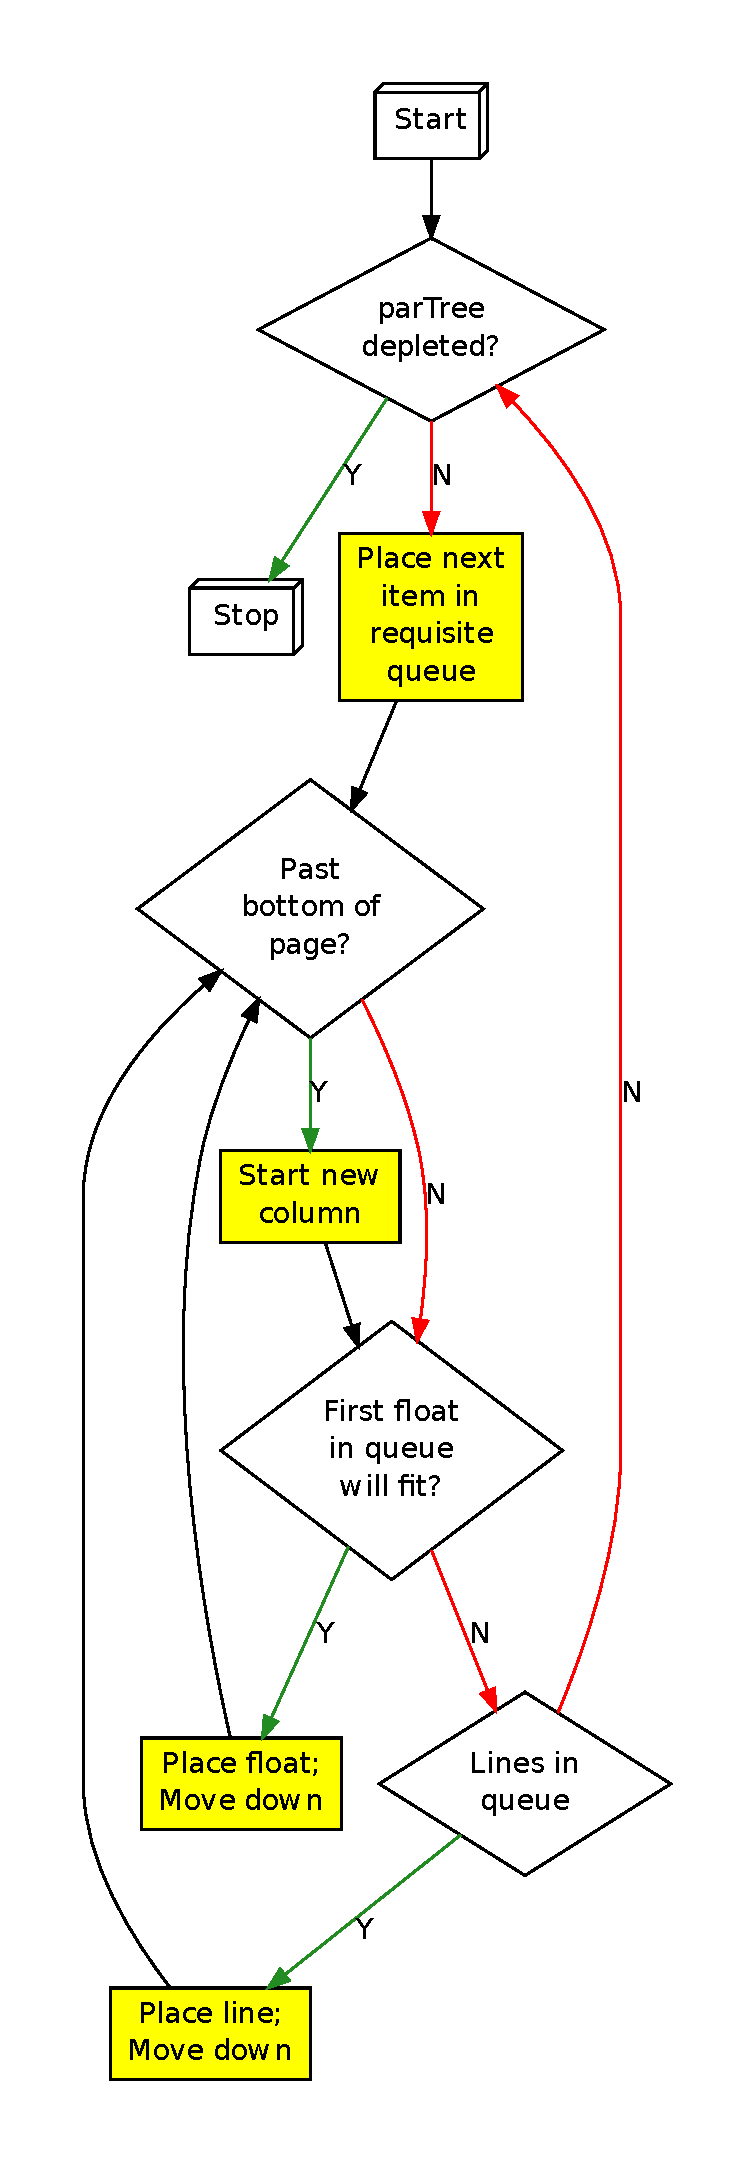
\includegraphics[height=\textheight]{gfx/floatqueueflowchart}
  \end{center}
  \caption[Flowchart of the two-queue float algorithm]{Flowchart describing the two-queue float algorithm}
  \label{fig:float-flowchart}
\end{figure}

Pagination is reasonably simple with this queueing system: as soon as a page is full, the layout can be restarted at the origin of the page using the current status of both queues and the Galley Structure Tree. It is entirely possible that floats may appear on pages subsequent to their callout point in the text, but this effect should be no worse than in many current typesetting systems.

Whilst this approach does produce reasonable layouts, and handles floats well without the need for backtracking, it is not particularly conducive to producing layouts with floats that span multiple columns. The queue-based layout described above is rather simplistic: it knows about the size of each component that it lays out, but it does not remember the history of the positions of any of the components that are already laid out. This makes it difficult to have items that span more than one column, because there is no mechanism to mark space on the page as being reserved. In order to do this, another approach must be taken.

\subsection{A Grid-Based Layout}
\label{sec:gridlayout}
% - Support of floats
    % - Queue system
    % - Grid/array system (no need for queue)
    % - Multicolumn floats
        % - issues with spanning \& pagination

\begin{figure}
    \includegraphics[width=\textwidth]{gfx/newspaper}
    \caption[An example of a grid-based layout]{An example of a grid-based layout in a UK newspaper. Note how all the baselines of the main body text are aligned to a common grid, and that all items span integer multiples of columns.}
    \label{fig:gridlayout}
\end{figure}

One method for allowing parts of a page to be reserved is to break it up into a grid. Grid-based layouts are useful in many situations;~\cite{Collier1991,Bringhurst2008} one example of particular note is that of modern-day newspapers (see figure~\ref{fig:gridlayout}). Following the example set by these newspapers, the grid used in this system is defined to have a row height of the \gls{leading} of the document's body text, and a column width of the \gls{measure} of one text column plus the required gutter space.



The viewer uses the dimensions of the float, as specified in the Galley Structure Tree (see Section~\ref{sec:docgen}), to determine how many columns it should span. The float is scaled to span the integer multiple of column widths that most closely matches its `natural' size, though for reasons that should hopefully be obvious, this number is limited to a minimum of 1, and a maximum of the number of columns on the page. Additionally, checks are made to ensure that the scaling will not cause the height of the figure to exceed that of the page.

An advantage of this grid-based approach is that it no longer requires the use of queues, either for lines, or for floats. The viewer simply traverses the Galley Structure Tree, placing each item in the first available place in the grid. In the case of floats, or other items larger than multiples of the main \gls{leading}, spaces in the grid can be marked as reserved, to prevent other items from trampling over their reserved space. If a float will not fit directly below the previous item to be placed, the grid is walked over until a gap of sufficient size can be found. Figure~\ref{fig:floatlayout} shows the progressive stages of this algorithm, and Figure~\ref{fig:screengrab} shows a real example of a document laid out with this system.

\begin{figure}
    \captionsetup[subfigure]{justification=raggedright}
    \subfloat[][Lines of text are added to the grid at the leftmost then topmost available position]{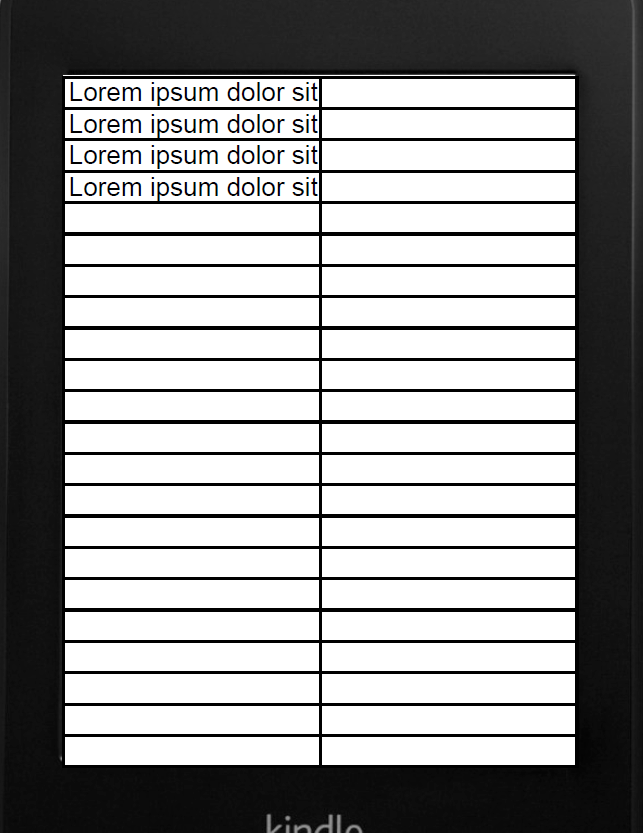
\includegraphics[width=0.3\textwidth]{gfx/float2.png}}\hspace{0.04\textwidth}
    \subfloat[][A 2-column float is encountered, and is inserted below the text]{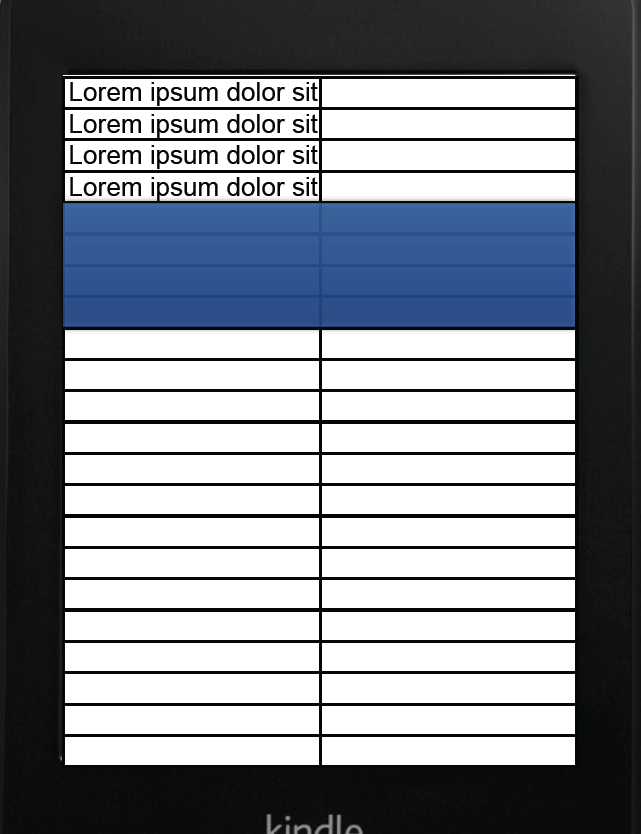
\includegraphics[width=0.3\textwidth]{gfx/float3.png}}\hspace{0.04\textwidth}
    \subfloat[][More lines of text are laid out]{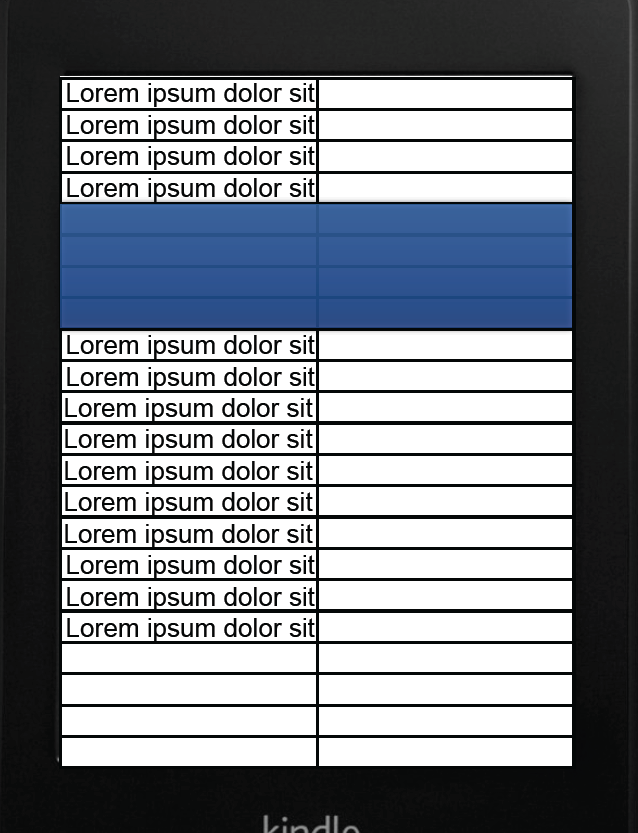
\includegraphics[width=0.3\textwidth]{gfx/float4.png}}\\
    \subfloat[][A single column float is encountered, but will not fit in the current space]{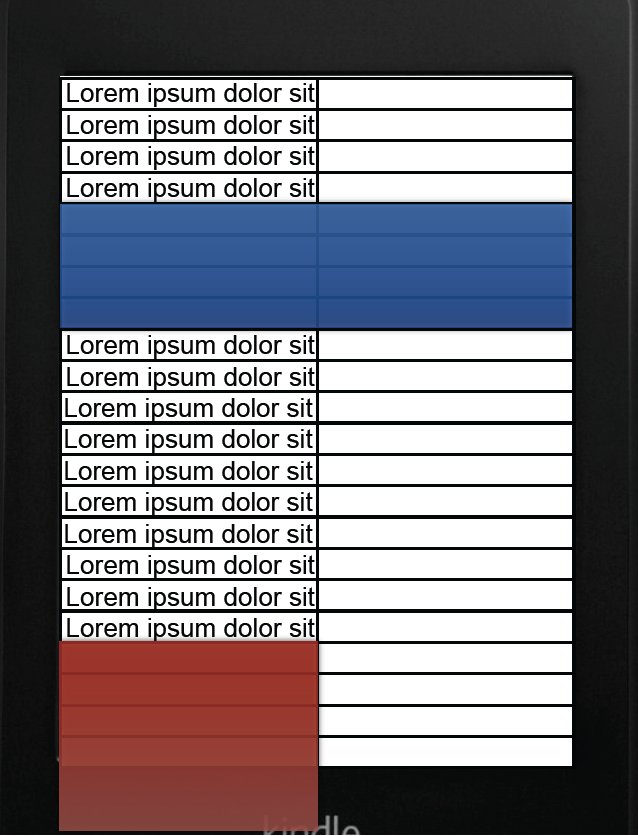
\includegraphics[width=0.3\textwidth]{gfx/float5.png}}\hspace{0.04\textwidth}
    \subfloat[][The float will also not fit at the top of the next column due to the position of the previous float]{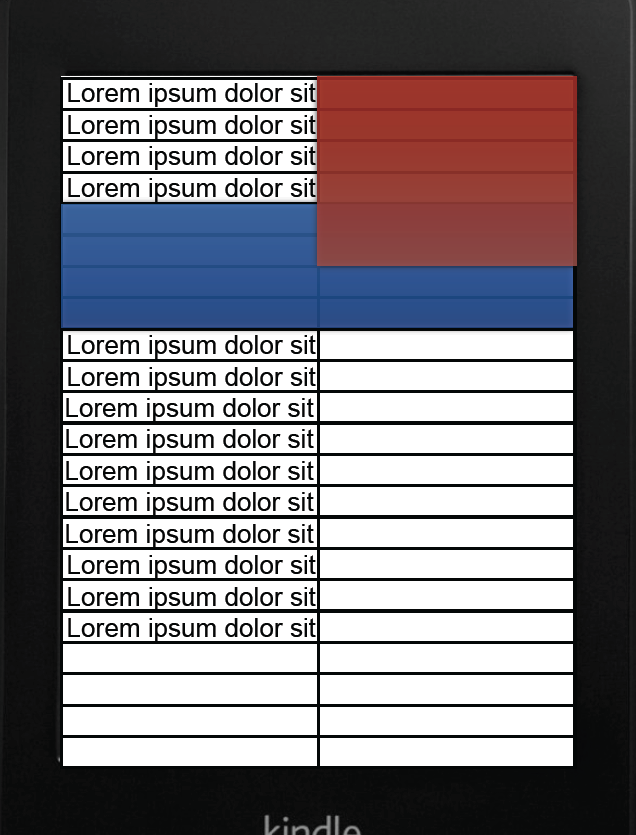
\includegraphics[width=0.3\textwidth]{gfx/float6.png}}\hspace{0.04\textwidth}
    \subfloat[][A space has been found for the second float]{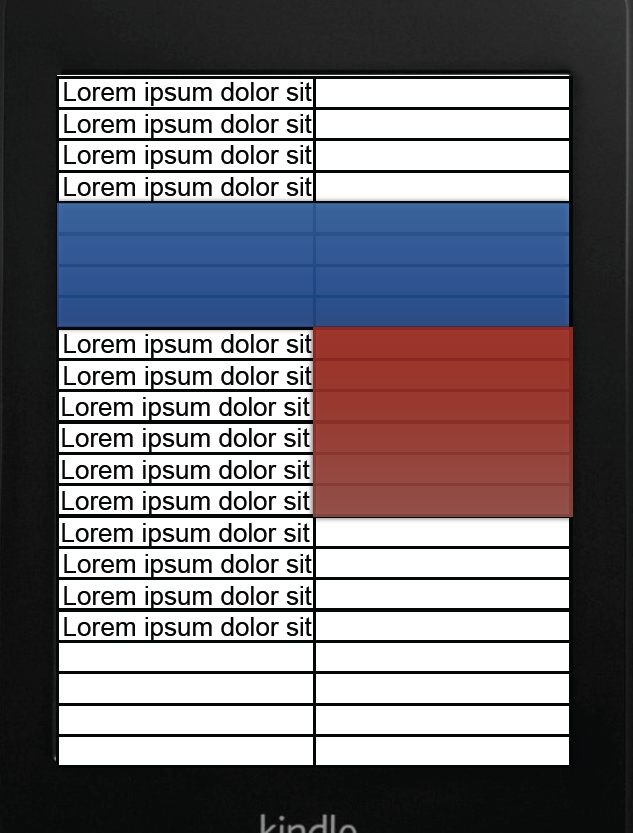
\includegraphics[width=0.3\textwidth]{gfx/float7.png}}\\
    \subfloat[][More text is laid out until the bottom of the column is reached]{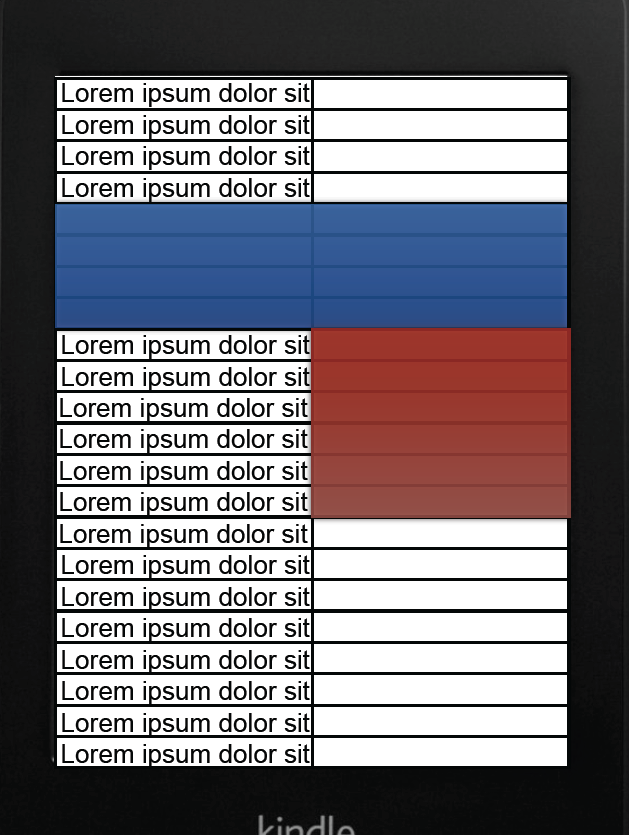
\includegraphics[width=0.3\textwidth]{gfx/float8.png}}\hspace{0.04\textwidth}
    \subfloat[][Text begins to be laid out at the top of the next column, until the reserved space of the float is encountered]{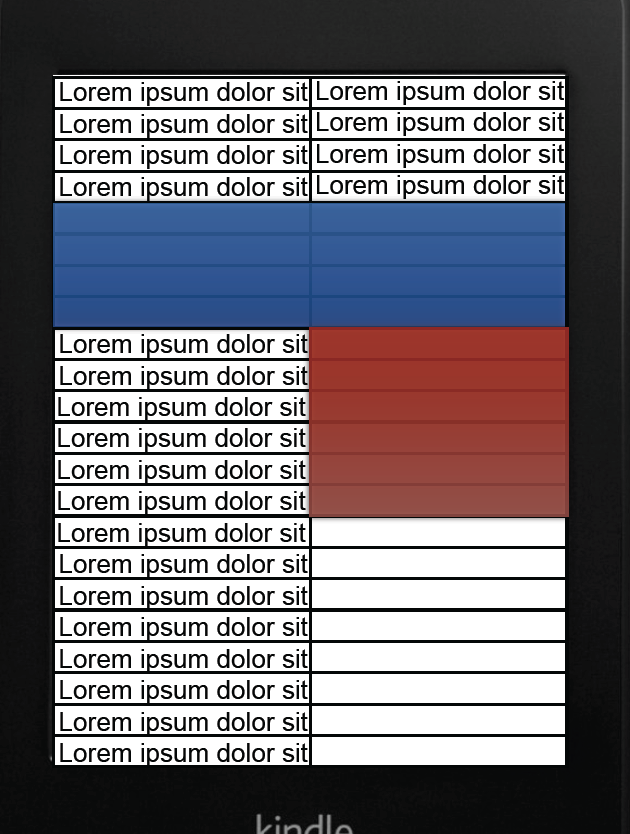
\includegraphics[width=0.3\textwidth]{gfx/float9.png}}\hspace{0.04\textwidth}
    \subfloat[][Text is subsequently laid out below the two floats until the page is filled]{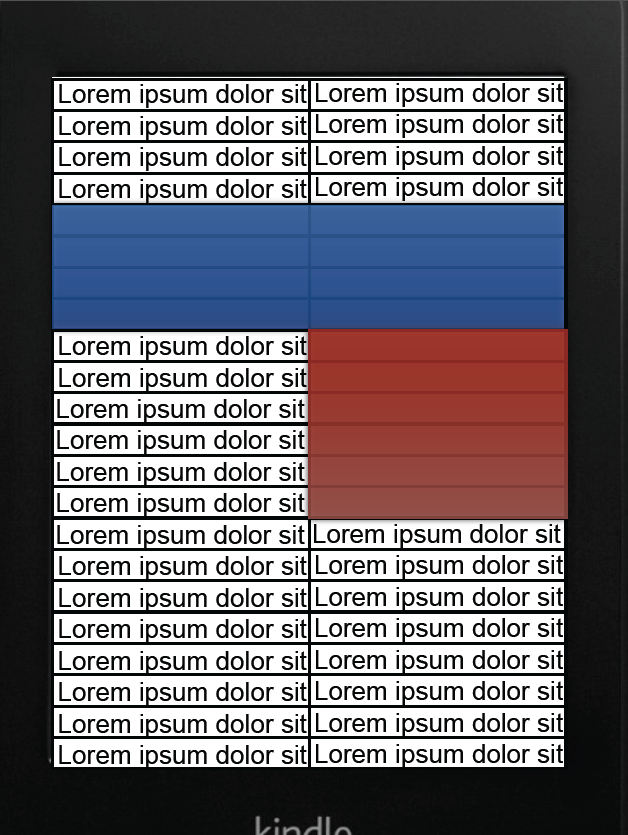
\includegraphics[width=0.3\textwidth]{gfx/float10.png}}
    \caption[Step through of multi-column layout]{A step-by-step example of how multi-column spanning floats are positioned using the grid-based layout described in Section~\ref{sec:gridlayout}}
    \label{fig:floatlayout}
\end{figure}



\begin{figure}
    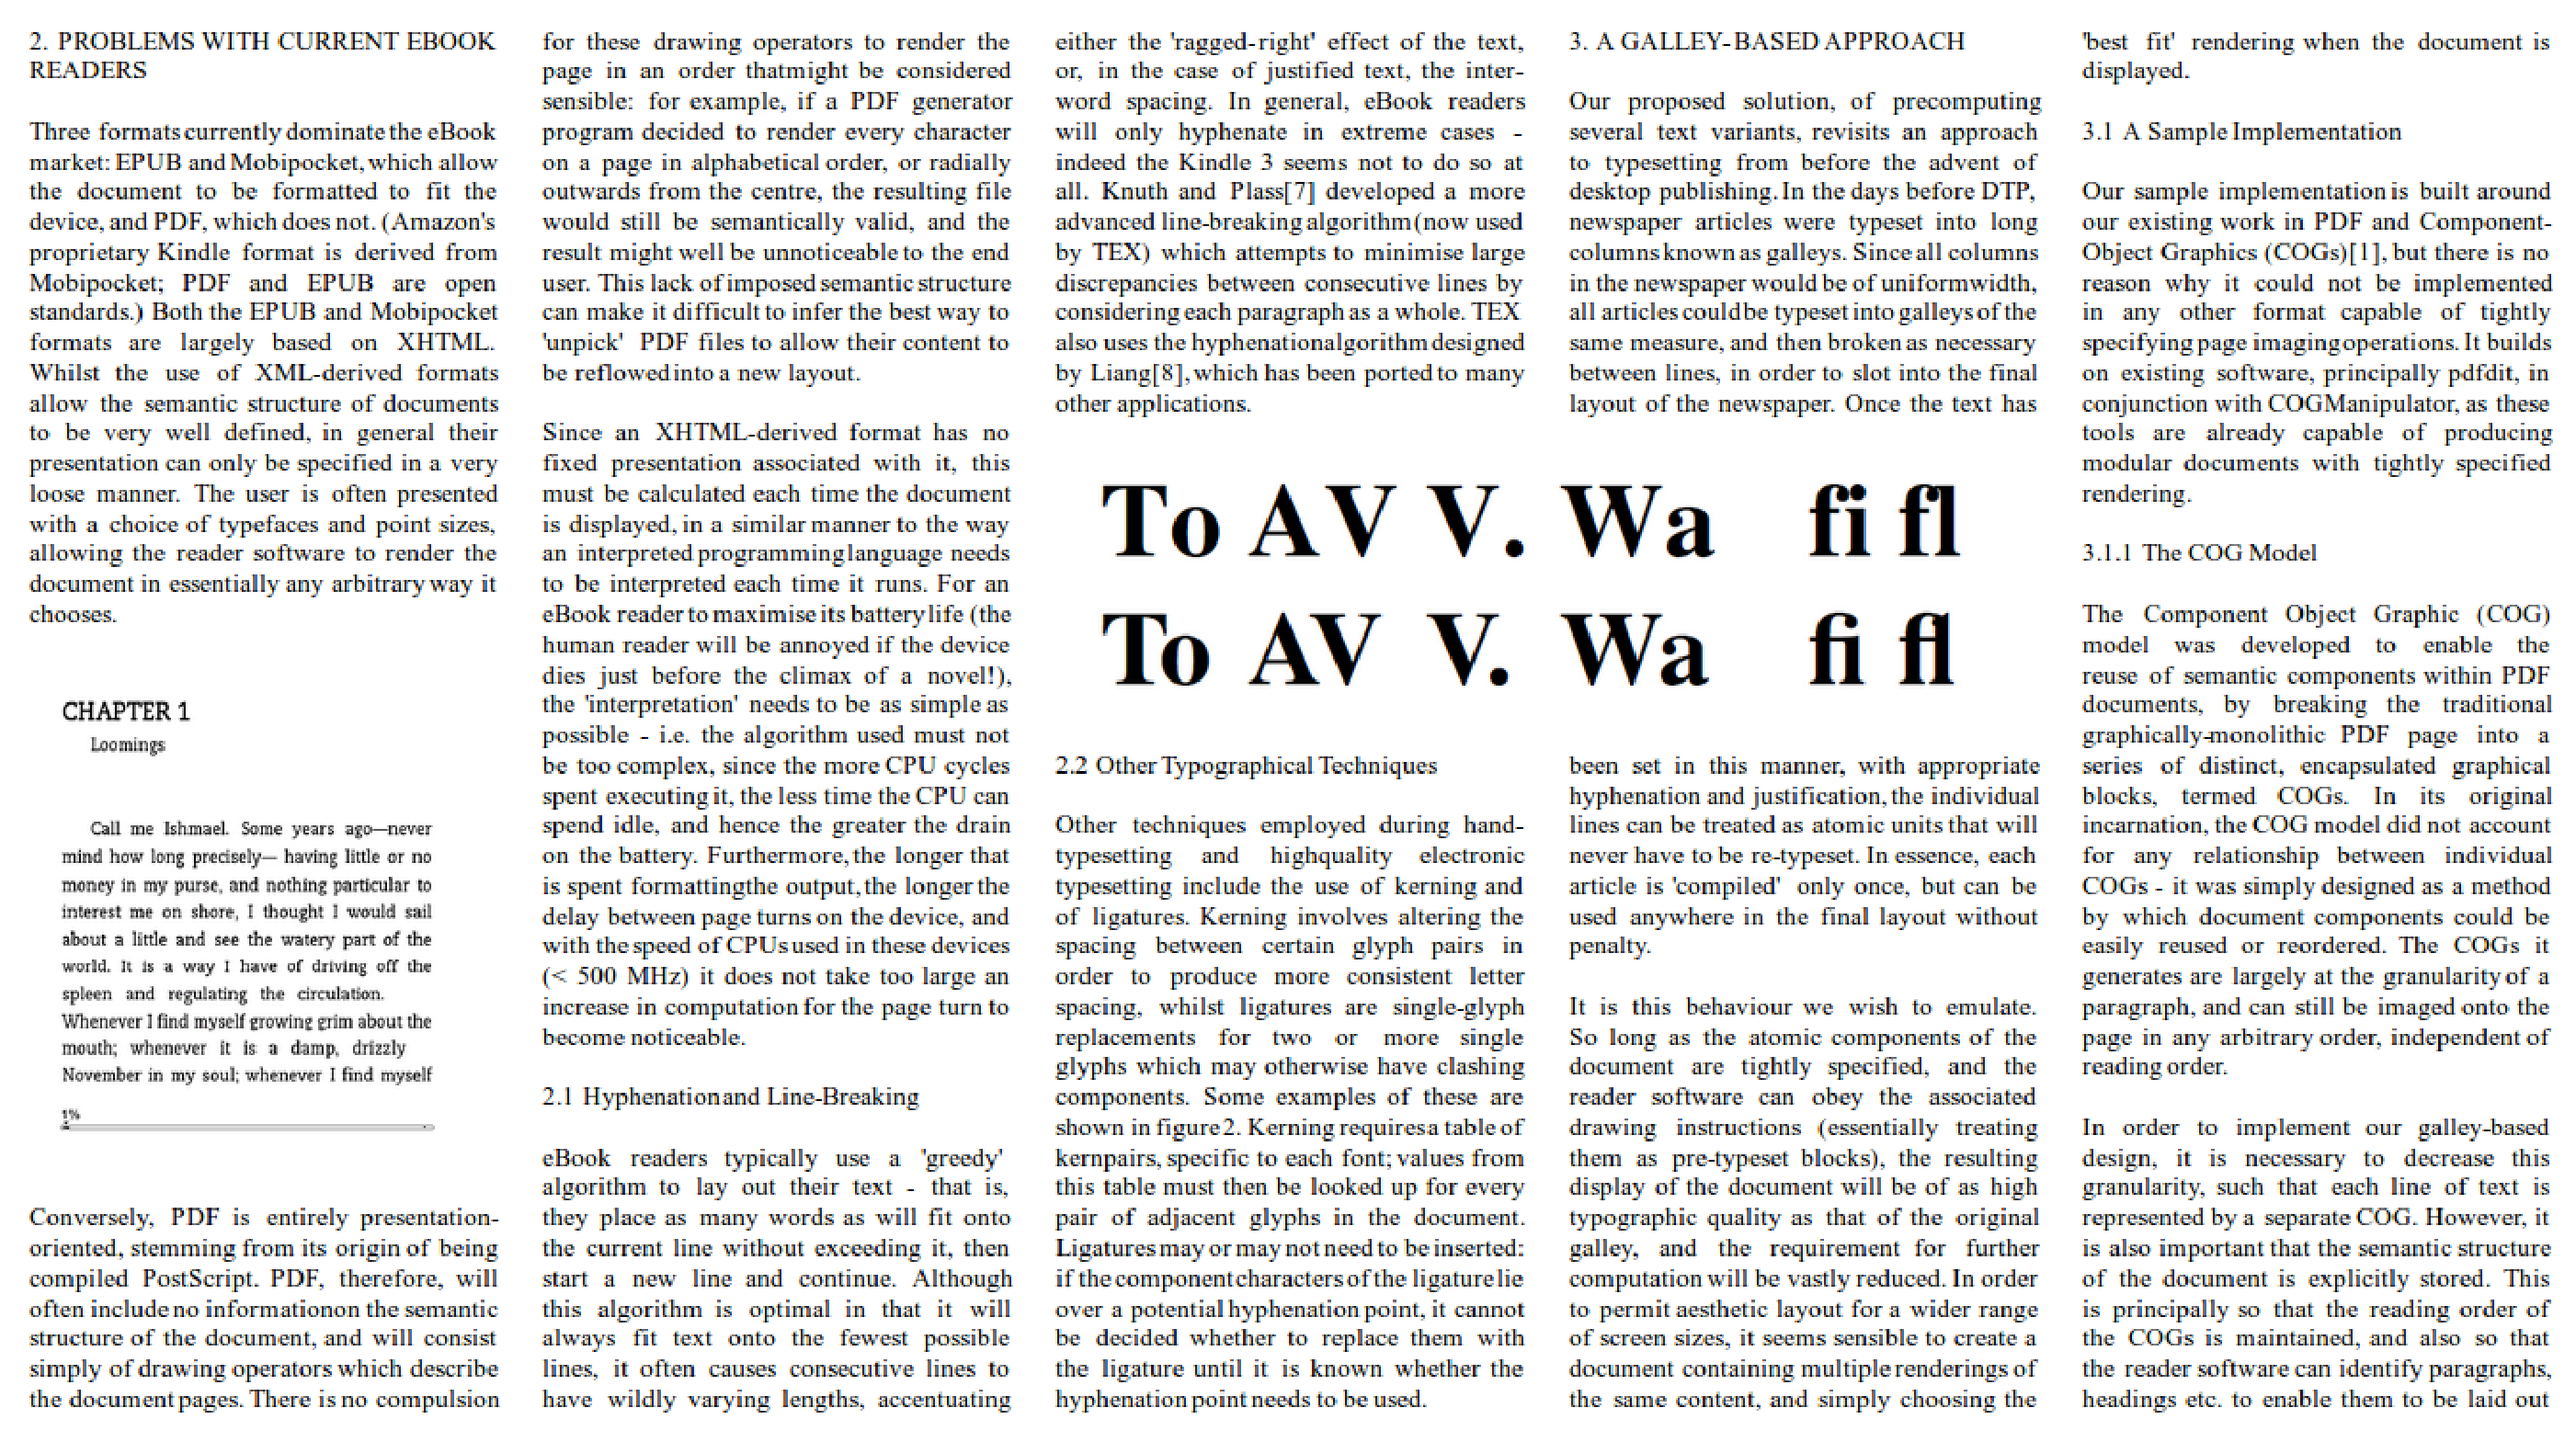
\includegraphics[angle=90,origin=c,width=\textwidth]{gfx/floatrendering}
    \caption[A sample rendering with multi-column floats]{An excerpt from \cite{Pinkney2011}, typeset and rendered by the system described in Chapter~\ref{ch:floats}. Of the two floats (a screenshot from a Kindle, and a demonstration of some micro-typographical techniques), one spans only one column, and one spans two. }
    \label{fig:screengrab}
\end{figure}


Pagination becomes a little trickier when floats are allowed to span multiple columns. For example, if a float whose natural size would lead it to span $n$ columns is encountered in the Galley Structure Tree when there are $(n-1)$ or fewer columns remaining to be typeset on the page, it must be decided how best to handle the situation. Three obvious options present themselves: alter the float to span fewer columns; delay the placement of the float until the start of the next page; or backtrack and check whether there is room to move the float back one or more columns, by shunting non-floatable text lines forwards.

The first option is clearly not ideal behaviour, given that shrinking a float may well reduce its legibility. Additionally, if this becomes a common problem, it is likely to be noticeable that floats spanning into the rightmost column of the page appear shrunken.

The second option (delaying placement until the following page) is a reasonable compromise, though it will increase float-drift (whereby floats become separated from their callout points in the text), which again is not ideal.

The third option (backtracking and shunting) is likely to produce the most desirable output, although some computational overhead will be added. One approach is simply to check whether there is enough space immediately to the left (specifically a gap between other, already placed, floats) into which the current float can be placed, with the displaced lines of text being shunted forwards. This method will not produce layouts as optimal as methods that use full backtracking and check all possibilities, but will run in much quicker time. A combination of all three of the above options is likely to work best in practice.


% \todo{Actually implement some of these pagination schemes, and write something intelligent-sounding about it. Provide some example output (screenshots).}

\section{Summary}

The reimplementation of the system in \html{} is not without its pitfalls. One strong advantage of using \pdf{} over \html{} is that any \pdf{} renderer that correctly implements the standard~\cite{Adobe2001} should display any given document in an identical manner to any other renderer. Regrettably (and much to the chagrin of web developers everywhere) this is very much not true of rival web browser layout engines. Though standards do exist, published by the \gls{w3c}, which are largely adhered to by all the major layout engines, there are certain areas that appear to be open to interpretation. One particular problem that is encountered, when using the system described in this chapter, is that of font scaling. 

The layouts produced by this system will only retain their quality if they are laid out precisely as specified by the typesetting process. Viewing the malleable documents in Google Chrome and Mozilla Firefox (which use WebKit and Gecko respectively) produces noticeably different results when the user chooses to scale the page up or down. WebKit appears to be inconsistent and non-linear when scaling fonts, whereas Gecko does a better job, and manages to lay out the text as intended by the typesetter. Figure~\ref{fig:craprenderer} shows an example of WebKit's font scaling problem. There is no real way around this issue, other than ensuring that whichever rendering engine is used in the reader device provides the required smooth scaling of fonts.

\begin{figure}
    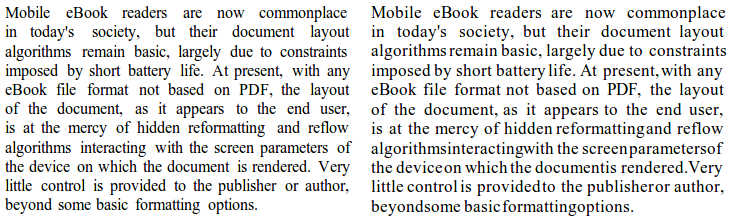
\includegraphics[width=\textwidth]{gfx/webkitisshit}
    \caption[Inconsistent font scaling by WebKit]{Chrome and Safari's layout engine (WebKit) can be inconsistent when scaling fonts. The paragraph to the left is displayed ``correctly'', but the paragraph to the right (scaled up by 1\% by the JavaScript) has clearly not scaled linearly. In contrast, Firefox's layout engine, Gecko, scales smoothly, and behaves as one might expect when zooming in on a \pdf{} file, which was the intended behaviour. (Output from Gecko is not shown in this figure.)}
    \label{fig:craprenderer}
\end{figure}


In general, however, as a document layout engine, the system produces pleasing-looking layouts that scale to fit on many different screen sizes, and the reimplementation in \textsc{xhtml}, \textsc{css}, and JavaScript makes the system much more portable. One stand-out problem remains: that of bloated filesizes. The next chapter suggests various methods to keep file sizes to a minimum.



%\todo{Write some analysis of the various float algorithms; provide some criticism of growing file sizes which leads onto the next chapter; mention problems that occur when the renderer tries to be clever (eg does its own kerning) ie Webkit vs Gecko}



\chapter{Dealing with File Bloat}\label{ch:bloat}

\summary{
In Chapter~\ref{ch:floats} we converted the implementation of our previously developed system into one that uses \html{}, \css{}, and JavaScript in place of \gls{pdf} and Adobe Acrobat, which vastly increases its portability. We also added support for floating items, which allows us to produce document layouts that are extremly similar to those used in newspapers, magazines, and academic journals.

In this chapter, we turn around and address the elephant in the room: what effect does the inclusion of all these renderings have upon file size, and what can we do about it?
}

\section{Rationale}
In the system described so far, the emphasis has been firmly upon reducing the computational complexity of layout operations at document view-time, and therefore little consideration has been given to the filesize of the output malleable documents.

%\todo{Put in some pdfdump output comparing ``normal'' pdfs with my malleable ones (maybe as an appendix)}

The tradeoff between filesize and required computation has previously been justified on the basis that storage is cheap,\marginpar{as of 2015, one US dollar will buy around three gigabytes of \textsc{nand} flash memory} light, and small, and that batteries, although relatively inexpensive, already comprise a significant portion of the overall mass and volume of most portable devices that are suitable for reading \ebook{}s. The consequence of this is that adding more storage would have little impact upon devices' aesthetics, but adding extra battery life (emerging nanotube battery technology notwithstanding) would result in vast increases in devices' overall bulk and mass.

Despite this, it seems perverse to make no attempt at all to keep filesizes as small as possible, as long as there are no (or limited) impacts upon the required computation at view-time.

Much like typesetting algorithms, few compression algorithms are designed with the minimisation of computation in mind. Consequently, the result of compressing the data using some generic algorithm is likely to require significantly more computation to decompress than a carefully designed bespoke algorithm. The following section describes work towards such an algorithm.


\section{Implementation}
The most obvious saving that can be made is with the duplication of a document's textual content. The systems described in Chapters \ref{ch:malleable}~and~\ref{ch:floats} both contain as many copies of the document text as there are pre-rendered galleys. In practice, there is no real need for more than one copy to be present in the file. Two approaches to this problem were considered.

\subsection{Pointers into the Source Text}
The first approach to be considered was to include the plaintext source of the document in its entirety, and for each rendering to contain only pointers to the relevant sections of text, instead of the words themselves. These pointers can either be absolute (in the form of a character offset from the start of the text) or logical (in the form \emph{paragraph m, word n}). If the document text is to be included as a plaintext string, absolute pointers are easier to use than logical: logical pointers require either an auxiliary data structure to map the logical pointers to absolute ones, or for the document text to be stored in a format reflecting the logical structure, \ie{} not in plain text.

The principal drawback of using this approach is that on occasion, the output of the linebreaking process does not precisely match the input: for example in the case where words are hyphenated (requiring one word to be broken into two parts, and the addition of a hyphen) or where certain glyphs may be substituted for others (such as with the use of ligatures, where a glyph pair or triplet may be replaced with a single glyph). For this reason, this approach was not considered further.


\subsection{Use of a Dictionary}
\label{sec:dictionary}
The second approach considered was the use of a dictionary to act as a lookup table for each word-level item produced by the linebreaking process.

A document's source text itself is likely to contain significant redundancy. In the 1930s, American linguist George Kingsley Zipf proposed \emph{Zipf's law},\hspace{0pt}\cite{zipf1932} which (broadly) states that given a sizeable sample of text in any given language, the frequency of any word is inversely proportional to its rank in the frequency table. Stated another way, the most common word tends to appear twice as often as the second most common word, three times as often as the third most common word, and so on. There have been many subsequent studies on redundancy in English that have come to related conclusions, for example Claude Shannon estimated the redundancy of written English to be around 50\%.\hspace{0pt}\cite{Shannon1951, Hirst1988}

\begin{sidewaystable} \footnotesize
    \myfloatalign
  \begin{tabular}{rrlrlrlrlrl} \toprule
    & \multicolumn{2}{l}{\textsc{Butterley}} & \multicolumn{2}{l}{\cite{Pinkney2011}} & \multicolumn{2}{l}{\textsc{Shakespeare}} & \multicolumn{2}{l}{\textsc{King James Bible}} & \multicolumn{2}{l}{\textsc{British National Corpus}}\\ 
    \midrule
		& $\numprint{103}$  & the       & $\numprint{233}$  & the      & $\numprint{23197}$  & the & $\numprint{62099}$  & the   & $\numprint{5375304}$  & the  \\ 
		& $\numprint{35}$   & of        & $\numprint{134}$  & of       & $\numprint{19540}$  & I   & $\numprint{38576}$  & and   & $\numprint{3010713}$  & of   \\ 
		& $\numprint{33}$   & and       & $\numprint{116}$  & to       & $\numprint{18263}$  & and & $\numprint{34445}$  & of    & $\numprint{2541227}$  & to   \\ 
		& $\numprint{31}$   & in        & $\numprint{75}$   & and      & $\numprint{15592}$  & to  & $\numprint{13387}$  & to    & $\numprint{2463817}$  & and  \\ 
		& $\numprint{25}$   & to        & $\numprint{75}$   & a        & $\numprint{15507}$  & of  & $\numprint{12735}$  & And   & $\numprint{2015815}$  & a    \\ 
		& $\numprint{23}$   & for       & $\numprint{56}$   & is       & $\numprint{12516}$  & a   & $\numprint{12451}$  & that  & $\numprint{1750205}$  & in   \\ 
		& $\numprint{23}$   & a         & $\numprint{52}$   & be       & $\numprint{10825}$  & my  & $\numprint{12167}$  & in    & $\numprint{949677}$   & that \\ 
		& $\numprint{21}$   & was       & $\numprint{50}$   & in       & $\numprint{9565}$   & in  & $\numprint{9760}$   & shall & $\numprint{924763}$   & is   \\ 
		& $\numprint{19}$   & company   & $\numprint{34}$   & as       & $\numprint{9059}$   & you & $\numprint{9508}$   & he    & $\numprint{838955}$   & was  \\ 
		& $\numprint{17}$   & Butterley & $\numprint{32}$   & document & $\numprint{7831}$   & is  & $\numprint{8932}$   & unto  & $\numprint{816193}$   & for  \\ 
    \midrule
    \textsc{total words}  & $\numprint{1232}$ & & $\numprint{3724}$ & & $\numprint{899595}$ & & $\numprint{821133}$ & & $\numprint{97087700}$ & \\ 
    \midrule
    \textsc{unique words} & $\numprint{628}$  & & $\numprint{1436}$ & & $\numprint{67107}$  & & $\numprint{33446}$  & & $\numprint{1733032}$  & \\ 
    \bottomrule    
  \end{tabular}
  \caption[Word frequencies in various documents]{Top 10 most frequent words in various documents. The total number of words and total unique words are also shown for each document. The data used to produce this table assumes a word is any contiguous block of (case-sensitive) non-whitespace characters; thus, ``\texttt{\textcolor{red}{and}}'' is distinct from ``\texttt{\textcolor{red}{And}}'', and ``\texttt{\textcolor{red}{document}}'' is distinct from ``\texttt{\textcolor{red}{document.}}''. The rationale behind this is that the data produced is more closely representative of a real dictionary of atomic ``words'' to be typeset in a malleable document.}
  \label{tab:wordfreq}
\end{sidewaystable}

\begin{figure}
  \begin{center}
  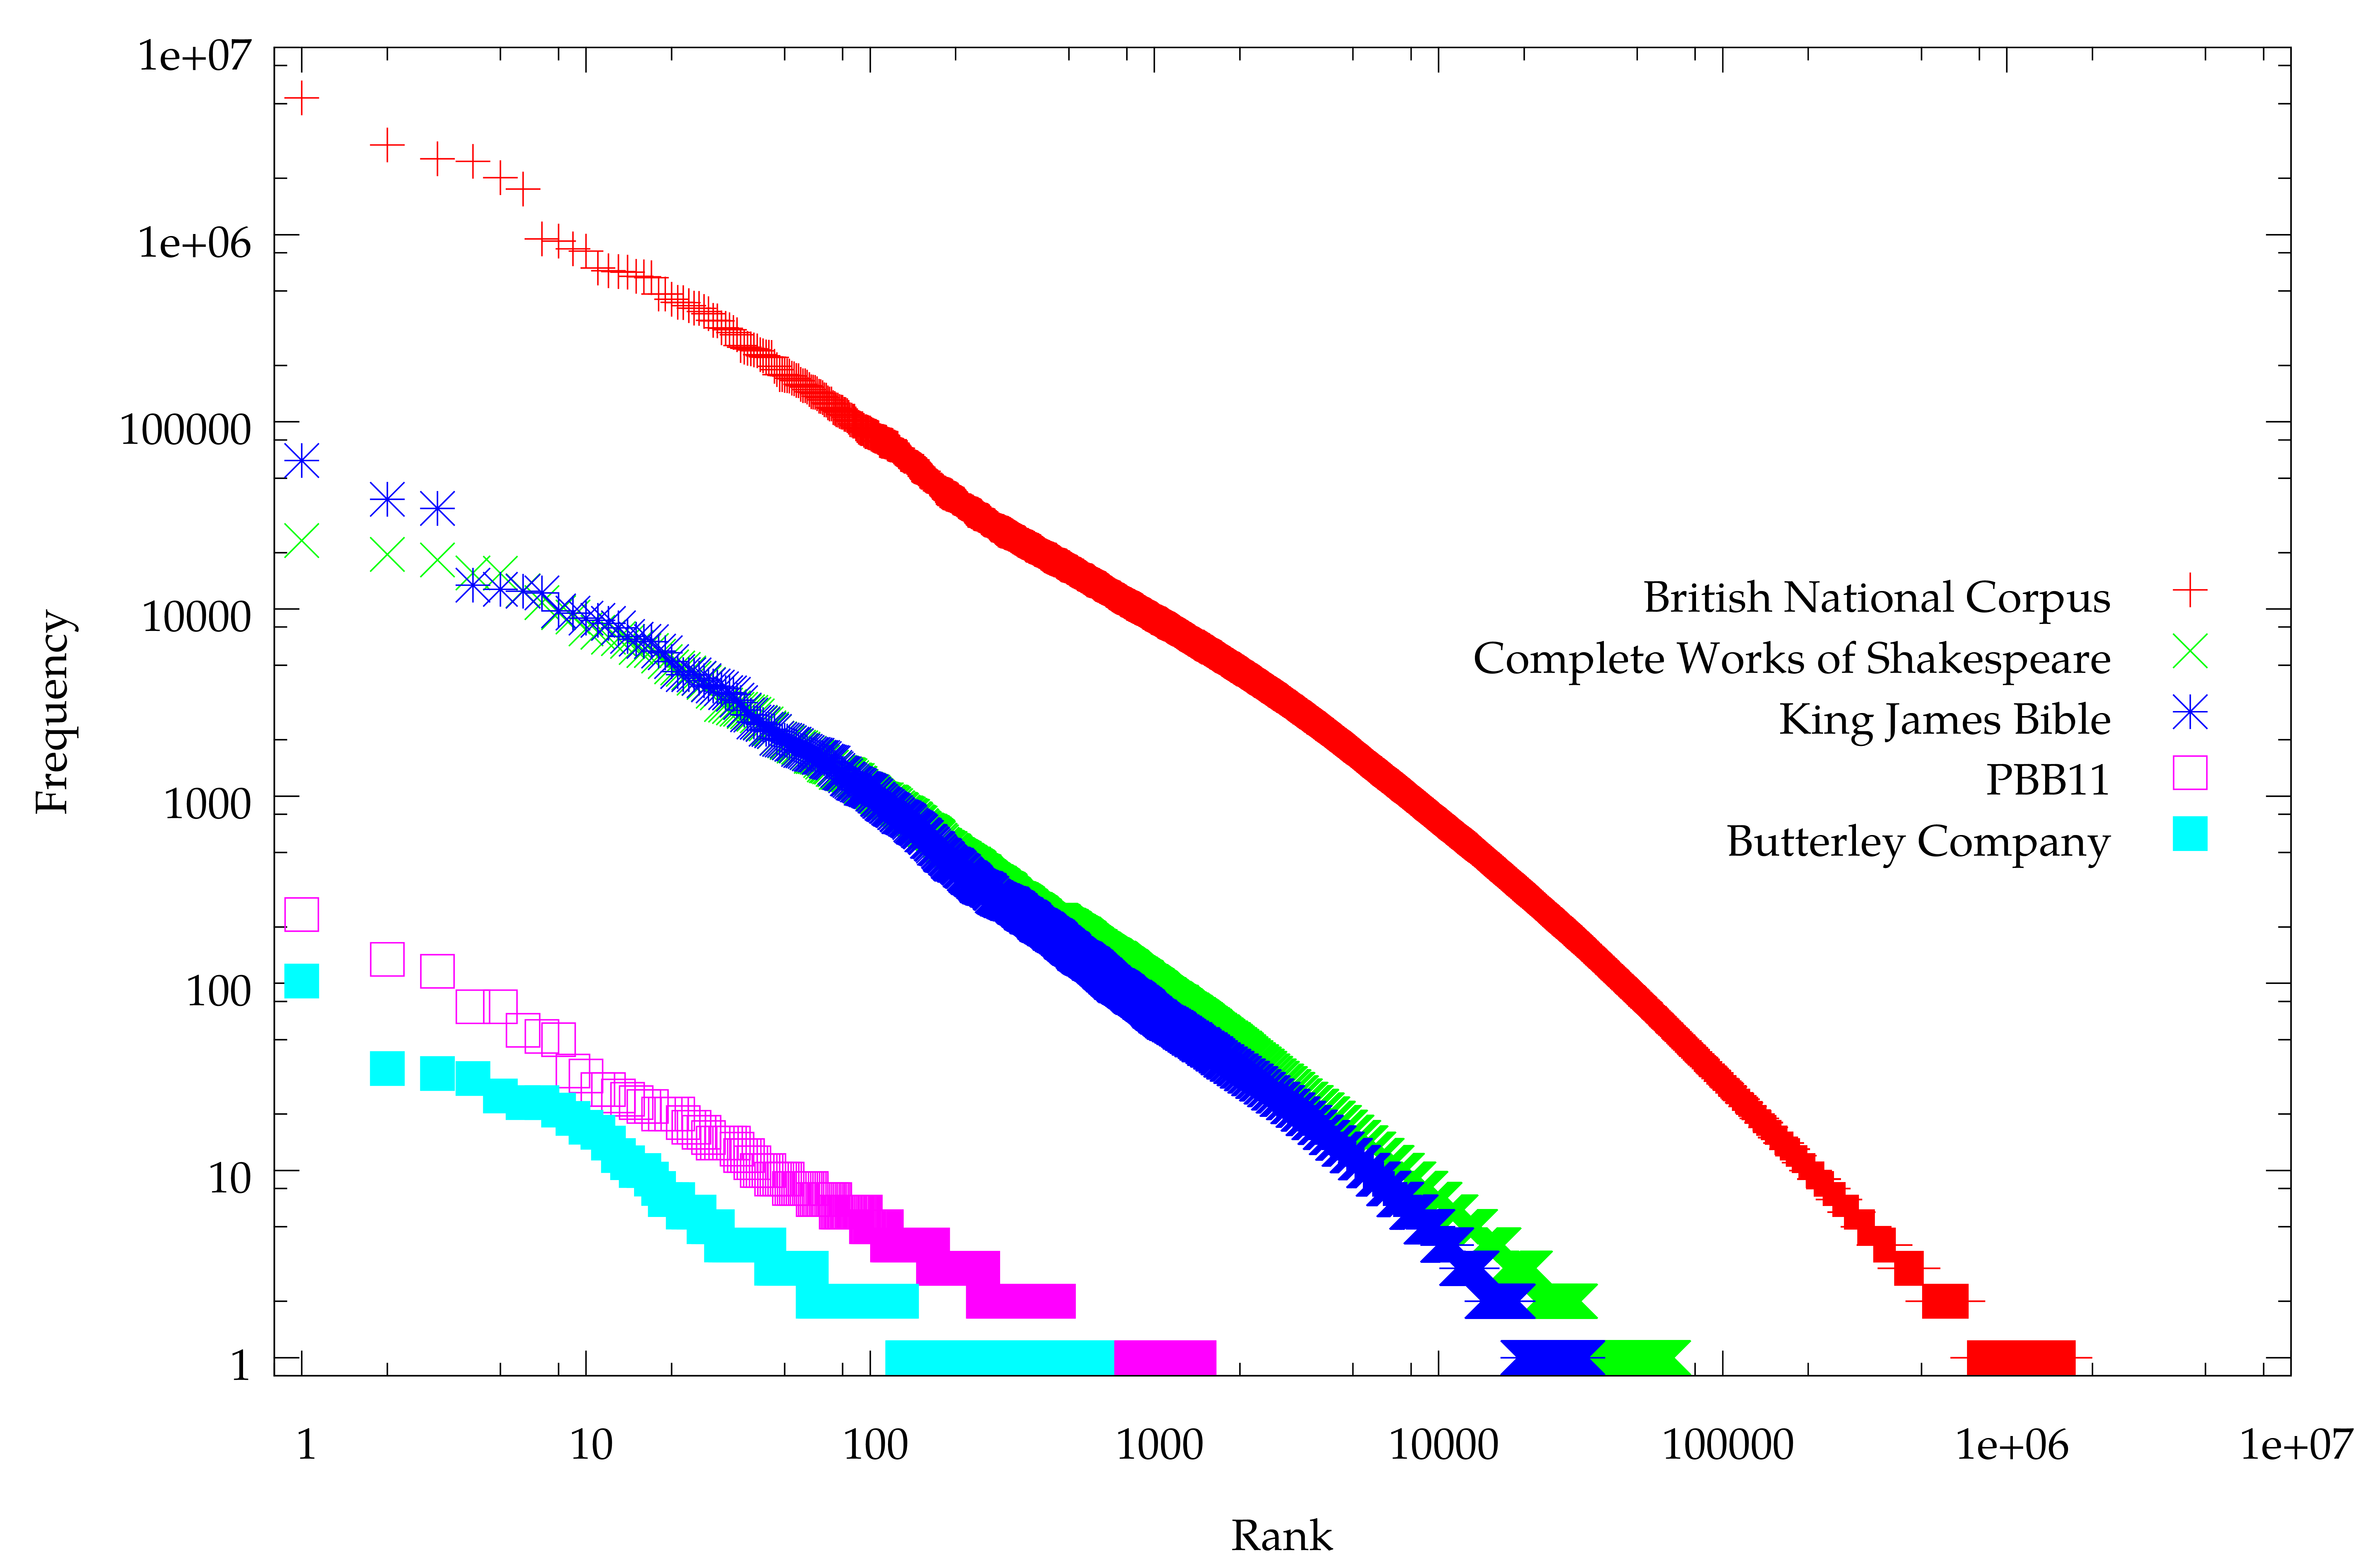
\includegraphics[width=\textwidth]{gnuplot/wordfreq-raster}
  \end{center}
  \caption[Word frequencies in various documents]{Word frequencies in various documents, plotted on a log-log scale. All of these documents, despite their varying lengths, appear to conform well with Zipf's Law, which manifests itself on a log-log scale as a straight line.}
  \label{fig:wordfreq}
\end{figure}

Table~\ref{tab:wordfreq} shows the ten most frequent words in four separate documents and for the British National Corpus\hspace{0pt}\cite{BNCConsortium2007} as a whole.\footnote{The British National Corpus describes itself as \emph{``a 100 million word collection of samples of written and spoken language from a wide range of sources, designed to represent a wide cross-section of British English from the later part of the 20th century, both spoken and written''} and is available freely online at \url{http://www.natcorp.ox.ac.uk/}} The four document used are the Wikipedia page for the \emph{Butterley Company}\footnote{\url{http://en.wikipedia.org/wiki/Butterley\_Company}}, the author's 2011 paper \emph{Reflowable Documents Composed from Pre-rendered Atomic Components}\hspace{0pt}\cite{Pinkney2011}, the Complete Works of Shakespeare,\marginpar{both Shakespeare and The Bible were obtained as plain text files from Project Gutenberg} and the King James Version of the Bible. Figure~\ref{fig:wordfreq} shows the word frequency data for the same documents plotted on a log-log scale. At the extremities, the data does not conform perfectly to Zipf's Law, though despite their hugely varying lengths, each document does display a clear Zipfian distribution.


This inherent redundancy in natural language can be exploited to produce a simple compression scheme through use of a dictionary. If, for example, the word ``shall'' appears multiple times in a document (in the King James Version of the Bible it appears 9760 times, and in the complete works of Shakespeare 3016 times) it is only stored once in the dictionary. As long as on average (\ie{} over every occurrence of every word) each word's key is lexicographically shorter than the word itself, it can be guaranteed that some redundancy has been removed from the data.

The \gls{html} and JavaScript system described in Chapter~\ref{ch:floats} can be altered to use a dictionary-based lookup table with fairly few modifications. Firstly, since the data for the malleable document must be represented in \gls{json},\footnote{see \url{http://www.json.org/} for full details} some means of including the dictionary must be devised. \gls{json} supports two types of collection. The first is the \emph{object}, which is defined formally as \emph{an \mbox{unordered} set of name/value pairs}. This acts much like an associative array, though it does not guarantee the order of its elements. The second collection type supported by \gls{json} is the \emph{array}, defined as \emph{an ordered collection of values}. Since both must be declared literally (in the forms \texttt{\{\textquotedbl key1\textquotedbl:\textquotedbl word1\textquotedbl,\textquotedbl key2\textquotedbl:\textquotedbl word2\textquotedbl\}} and \texttt{[\textquotedbl word1\textquotedbl,\textquotedbl word2\textquotedbl]} respectively) rather than being populated programatically, using a plain array for the dictionary allows us to omit the keys from the dictionary itself, as they are implied by the order of the elements in the array. Additionally, since this forces the use of integers as keys, the Galley Structure Tree will not require the use of quote marks when the dictionary keys are referenced. If the keys were string values, each use of each key in the Galley Structure Tree would therefore necessitate two extra characters (\eg{} \texttt{\textquotedbl key\textquotedbl} versus \texttt{401}).

It should also be noted that using integers as keys in \gls{json} has different implications to using integers as keys in some more compact binary format. \gls{json} is always stored in some textual encoding (perhaps \textsc{ascii}, perhaps \textsc{utf-8}), and there is no support for numeric representation in any base other than decimal. What might take up one 32 bit integer (\ie{} 4 bytes) in a compiled language such as C might take as many as ten textual characters (10 bytes, assuming that whichever character encoding system is used represents low-\textsc{ascii} characters with only one byte). Conversely, textual representation of integers can be more compact under certain conditions: namely, for values that use three or fewer characters, \ie{} the numbers 0--999.

\begin{figure}
  \begin{center}
  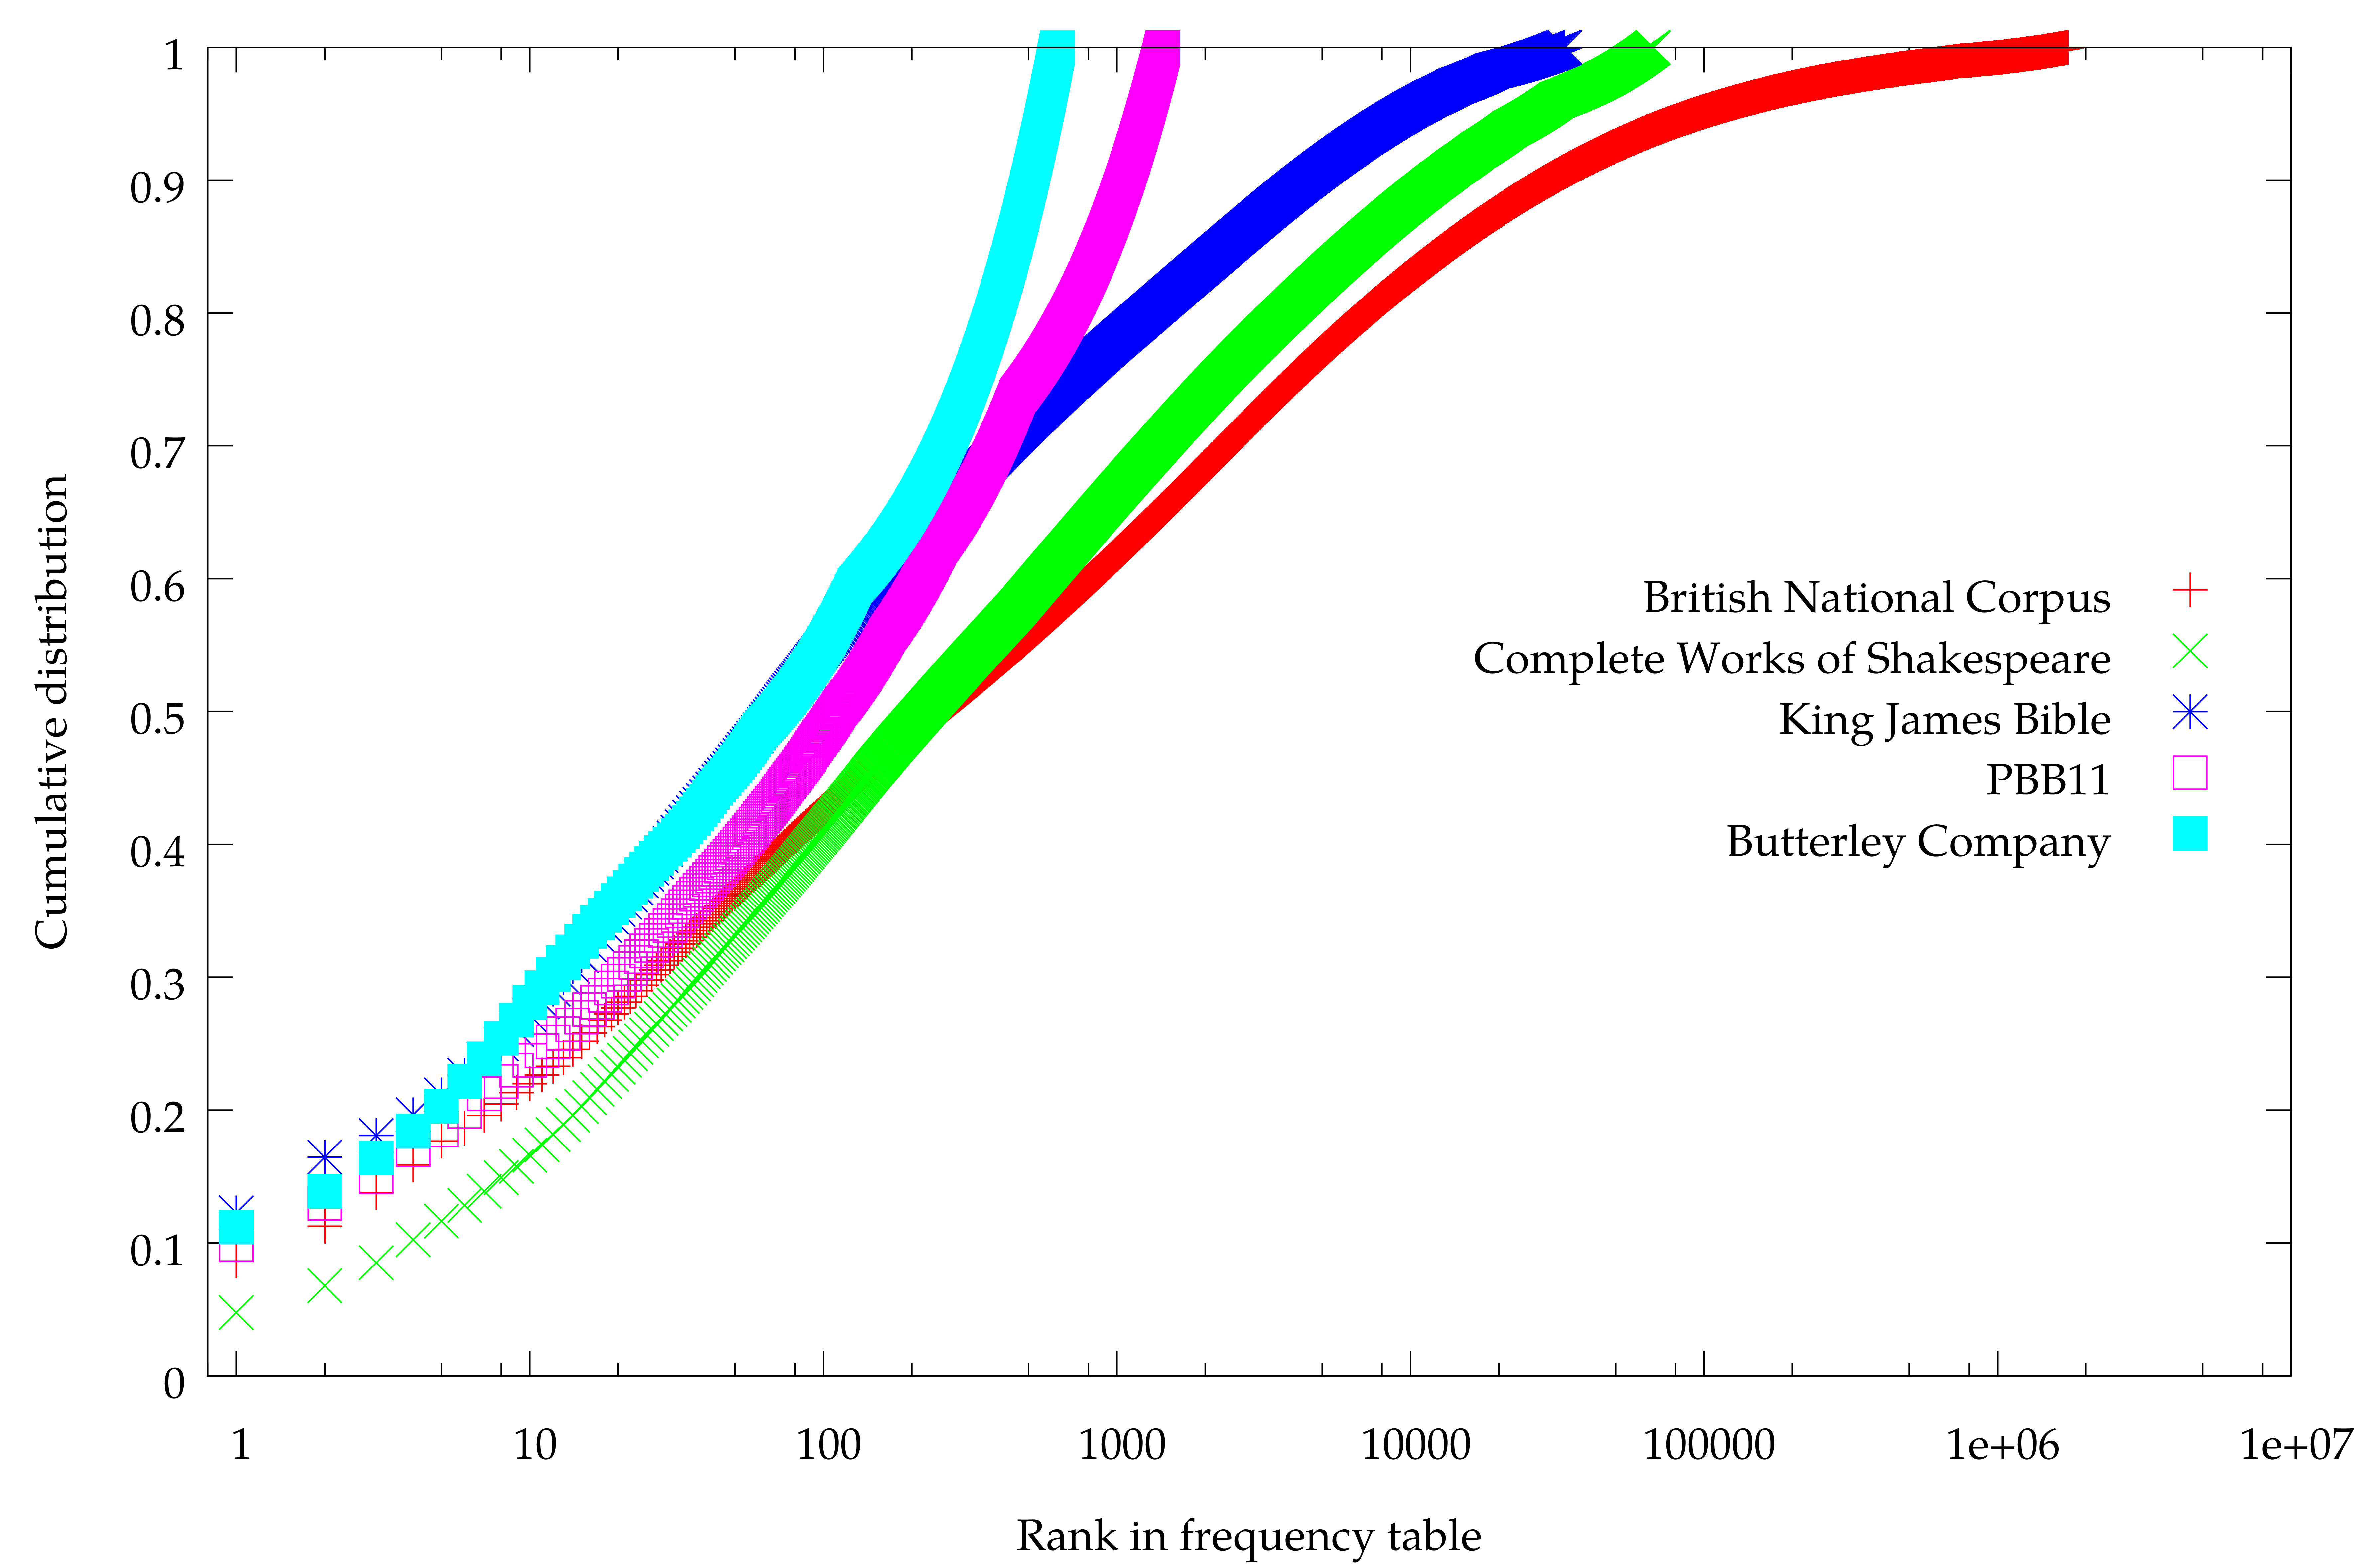
\includegraphics[width=\textwidth]{gnuplot/cumulative-raster}
  \end{center}
  \caption[Cumulative distribution of word frequencies]{Cumulative distribution of word frequencies in various documents. }
  \label{fig:cumulative}
\end{figure}

Referring back to Figure \ref{fig:wordfreq}, to Figure~\ref{fig:cumulative}, and to Zipf's law, it can be seen that even for extremely long documents, the number of words that are ranked in the top 1000 exceeds 60\%, and so as long as the order of words in the dictionary is chosen carefully, using a textual representation of integers can be more compact than a na\"ive binary representation.

It was therefore decided to store the dictionary as an array, ordered such that the most frequently occurring words have the shortest keys.

\subsection{Further Compression Possibilities}
\label{sec:deltas}

The techniques discussed thus far have focused mostly upon exploiting the inherent redundancy in natural language. A fairly large part of the data contained within the Galley Structure Tree has been overlooked: the typesetting data itself.

All of the aforementioned encoding systems have used an absolute value for the x position of each word on each line; that is, each occurrence of each word has an associated value representing the required distance of its placement, in \glspl{point}, from the start of the line. An example of this can be seen in Listing~\ref{lst:datajs} on page~\pageref{lst:datajs}.

With a view to producing data that would be more easily compressible by a generic compression algorithm (that would perhaps be useful if \textsc{HTTP} compression or similar is used to transfer the document data to a device) it was decided to investigate a different approach to storing this data.

In any typeset document, most (if not all) occurrences of the same word will typeset identically upon the page. In particular, the amount of horizontal space reserved for a word will be the same for each occurrence of the word. Similarly, if a document's text is fully justified, the space between words on each individual line will be identical. If the document is left-justified, then each space between each pair of words on \emph{every} line will be identical. This redundancy is present within all the previous encodings, but cannot be picked up by a generic compression algorithm, since it requires knowledge of the typesetting process. By separating the word widths from the spacing, this redundancy can be made more explicit, and therefore easier for a generic compression algorithm to take advantage of.

\begin{lstlisting}[label=lst:deltasdata,captionpos=b,float,language=c,stringstyle=\color{blue},basicstyle=\ttfamily\footnotesize,caption={[Excerpt from a paragraph tree using deltas]Excerpt from a JavaScript data file that uses position deltas in the Galley Structure Tree, representing one galley rendering of one paragraph. The first value in each pair is the position delta (in points) and the second is the dictionary key of the associated word.}]
[
    [[0,982],[3.678,26],[3.678,93]],
    [[0,14],[2.682,1307],[2.682,558]],
    [[0,7],[3.668,557],[3.668,797],[3.668,226]],
    [[0,102],[4.338,9],[4.338,30]],
    [[0,112],[2.4,1013],[2.4,1068]],
    [[0,182],[2.4,1303],[2.4,2],[2.4,547]],
    [[0,308],[15.666,15],[15.666,1114]],
    [[0,177],[2.4,1173],[2.4,229],[2.4,733]],
    [[0,19],[7.336,81],[7.336,26],[7.336,143]],
    [[0,96],[7.116,33],[7.116,97],[7.116,16]],
    [[0,141],[9.444,0],[9.444,30],[9.444,1]],
    [[0,0],[8.78,89],[8.78,8],[8.78,11]],
    [[0,905],[10.008,2],[10.008,0],[10.008,66]],
    [[0,1125],[5.922,5],[5.922,34],[5.922,0],[5.922,1172]],
    [[0,1],[2.676,1053],[2.676,471]],
    [[0,3],[4.008,967],[4.008,112]],
    [[0,524],[10.338,19],[10.338,0]],
    [[0,126],[7.356,571],[7.356,1]],
    [[0,0],[6.896,197],[6.896,16],[6.896,18]],
    [[0,0],[2.4,9],[2.4,5],[2.4,691]],
    [[0,1249],[14.004,1046],[14.004,317]],
    [[0,5],[11.112,289],[11.112,2],[11.112,0]],
    [[0,273],[9.84,24],[9.84,859]],
    [[0,986],[11.34,144],[11.34,210]],
    [[0,263],[2.4,774]]
],
\end{lstlisting}

\begin{lstlisting}[label=lst:deltasdict,captionpos=b,float,language=c,stringstyle=\color{blue},basicstyle=\ttfamily\footnotesize,caption={[Excerpt from a dictionary storing word widths]Excerpt from the dictionary from a JavaScript data file that uses position deltas, where the width of each word is stored alongside the word itself. This is the dictionary from a rendering of \cite{Pinkney2011}: compare its ordering to that shown in Table~\ref{tab:wordfreq} on page~\pageref{tab:wordfreq}.}]
 [["the",14.664],["of",9.996],["to",9.336],["and",17.328],["a",5.328],["is",8.004],["be",11.328],["in",9.336],["as",9.996],["document",47.328],["that",18],["it",6.672],["page",22.656],["for",13.992],["are",14.652],["by",12],["on",12],["will",18.672],["which",29.328],["with",21.336],["this",17.34],["The",18.66],["can",16.656],["an",11.328],["or",9.996],["-",3.996],["eBook",31.332],["used",21.996],["PDF",22.008],["In",9.996],["layout",30],["have",22.656],["from",23.328],["not",15.336],["at",8.664],["width",27.336],["This",21.336],["has",15.996],["then",20.664],["each",21.984],["was",18.66],["typesetting",52.668],["columns",40.668],["simply",32.676],["these",24.66],["text",18],["into",18.672],["hyphenation",59.328],["content",35.328],["quality",33.336],["column",36],["lines",22.668],["only",21.336],["line",18],["ACM",27.336],["our",15.996],["its",11.34],["structure",41.988],["Document",49.992],["penalty",35.328],["between",39.984],["galley",29.328],["order",25.32],["more",24.66],["COGs",30],["out",15.336],["end",17.328],["one",17.328],["use",15.996],["algorithm",46.668],["producing",48.66],["columns.",43.668],["galleys",33.996],["figure",28.656],["simple",32.004],["would",30],
\end{lstlisting}

On the basis of the above observations, the decision was taken that the dictionary should be modified to store the width of each word alongside itself, and that the Galley Structure Tree should be modified so that each word to be typeset is now accompanied by the offset required from the end of the previous word (which will henceforth be referred to as \emph{position deltas}) rather than the absolute offset required from the start of the line. This does of course necessitate two array lookups in the dictionary where previously there would have been one, but since array accesses run in constant time, this does not present a problem. Excerpts from a Galley Structure Tree and dictionary that use this encoding system are shown in Listings \ref{lst:deltasdata}~and~\ref{lst:deltasdict} respectively.

Further redundancy could be removed by exploiting the fact that words tend to be regularly spaced on each line. Whilst the encoding could be modified to allow only regular spacing of words, it was felt that this might be somewhat restrictive, and would detract from the appeal of the system as something that supports complex, arbitrary layouts.

Even without making further compression attempts beyond the encoding system shown in Listings \ref{lst:deltasdata}~and~\ref{lst:deltasdict}\ed the motivation for which, we must remember, was to produce an encoding that was more \emph{compressible}, rather than more \emph{compressed}\ed by pure chance, it turns out that even in its full form, this is the most compact representation yet devised!



\section{Results}

The following pages show the evolution of the encoding system, and how the filesizes vary according to the number of included galley renderings, for the same sample documents that are used for Figures \ref{fig:wordfreq}~and~\ref{fig:cumulative}:

\begin{itemize}

 \item Figure~\ref{fig:size-json} (page~\pageref{fig:size-json}) shows the ``original'' encoding system described in Chapter~\ref{ch:floats}, which does not make any attempt to minimise filesize.

 \item Figure~\ref{fig:size-unord} (page~\pageref{fig:size-unord}) shows the encoding system described in Section~\ref{sec:dictionary}, using a dictionary ordered such that the earliest occurring words have the shortest keys. (The dictionary is therefore described as \emph{unordered}.)

 \item Figure~\ref{fig:size-ord} (page~\pageref{fig:size-ord}) shows the encoding system described in Section~\ref{sec:dictionary}, using a dictionary ordered such that the most frequently occurring words have the shortest keys. (The dictionary is therefore described as \emph{ordered}.)

 \item Figure~\ref{fig:size-deltas} (page~\pageref{fig:size-deltas}) shows the encoding system described in Section~\ref{sec:deltas}, which not only uses a dictionary ordered such that the most frequently occurring words have the shortest keys, but also stores the width of each word in the dictionary, so that the Galley Structure Tree contains deltas rather than absolute positioning data.
 
 \item Figure~\ref{fig:size-all-b} (page~\pageref{fig:size-all-b}) shows a comparison of the filesizes produced by all encodings, and Figure~\ref{fig:size-all-gz} (page~\pageref{fig:size-all-gz}) shows the resultant filesizes when each rendering is further compressed with \texttt{gzip}.
\end{itemize}


\begin{figure}
  \begin{center}
  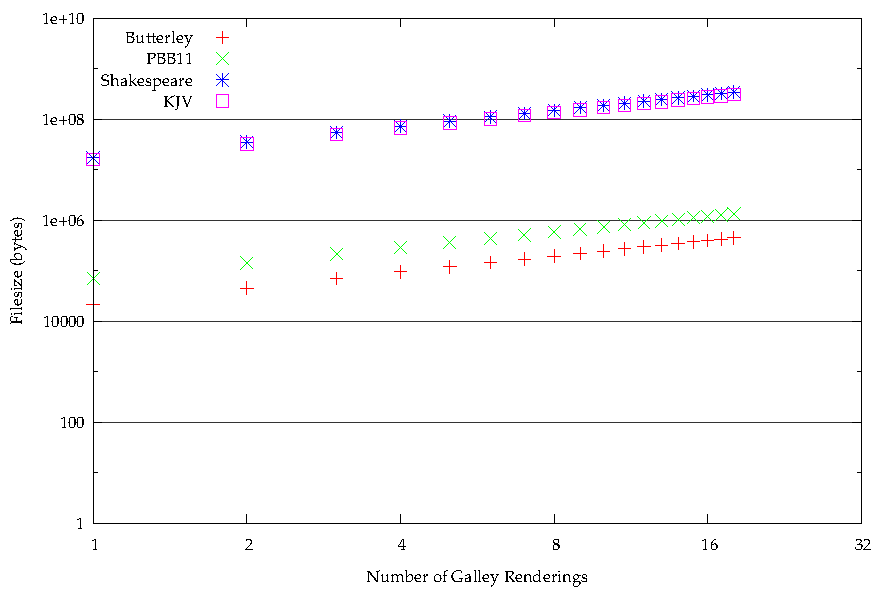
\includegraphics[width=\textwidth]{gnuplot/2-b}
  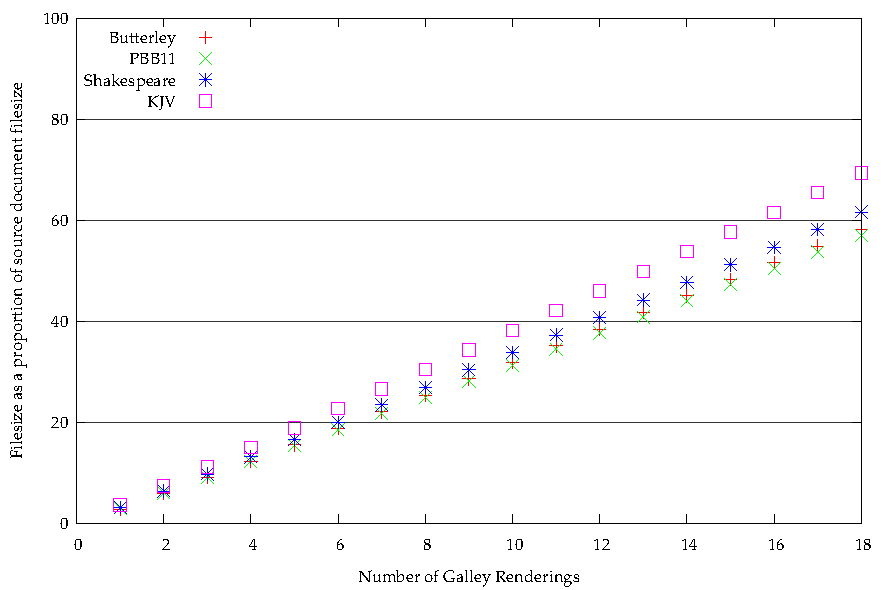
\includegraphics[width=\textwidth]{gnuplot/2-s}
  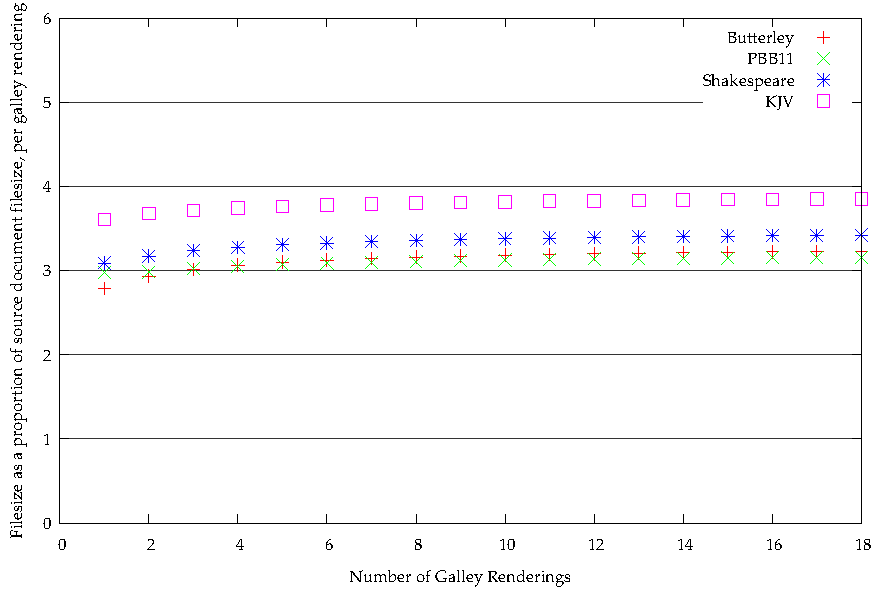
\includegraphics[width=\textwidth]{gnuplot/2-r}
  \end{center}
  \caption[Filesizes of documents in original encoding]{Filesizes of various documents, using the original encoding.}
  \label{fig:size-json}
\end{figure}



\begin{figure}
  \begin{center}
  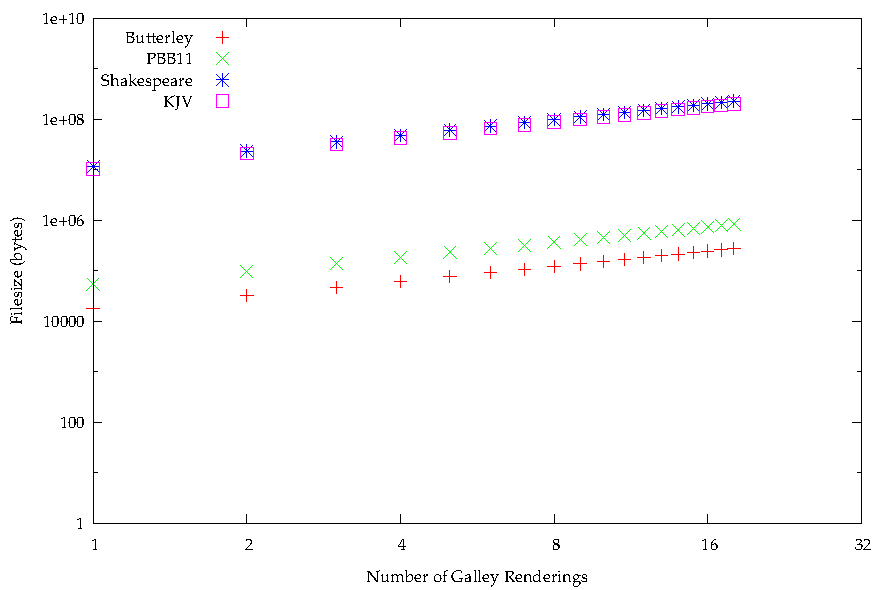
\includegraphics[width=\textwidth]{gnuplot/3-b}
  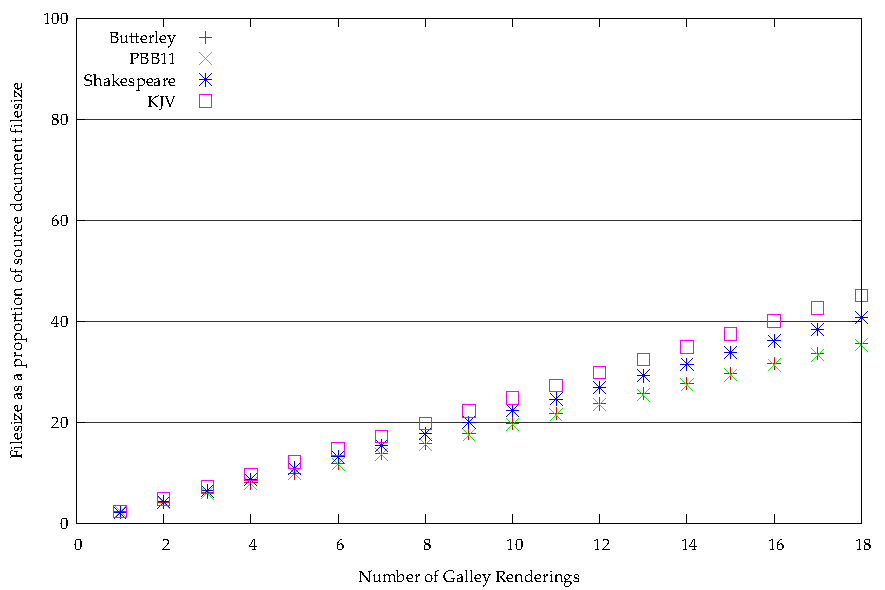
\includegraphics[width=\textwidth]{gnuplot/3-s}
  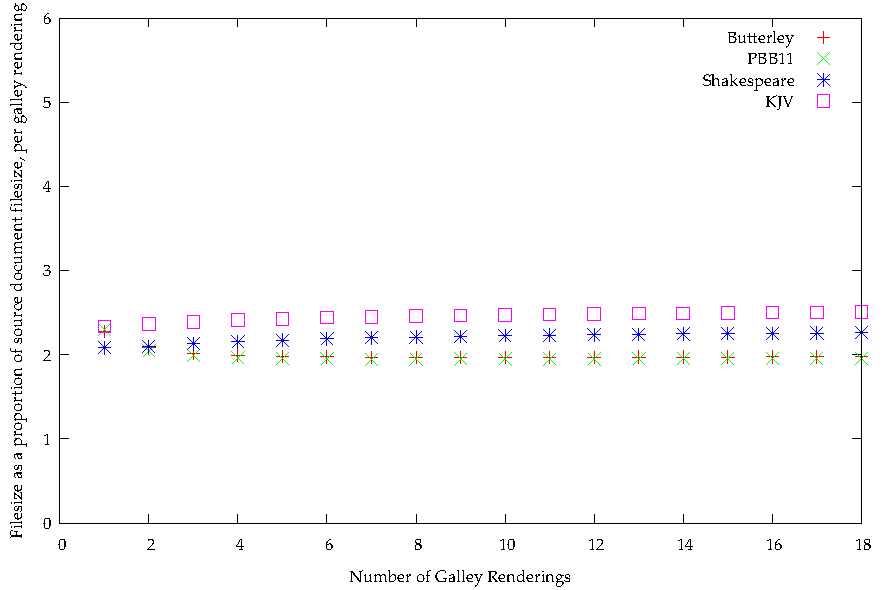
\includegraphics[width=\textwidth]{gnuplot/3-r}
  \end{center}
  \caption[Filesizes with an unordered dictionary]{Filesizes of various documents, encoded using an unordered dictionary.}
  \label{fig:size-unord}
\end{figure}



\begin{figure}
  \begin{center}
  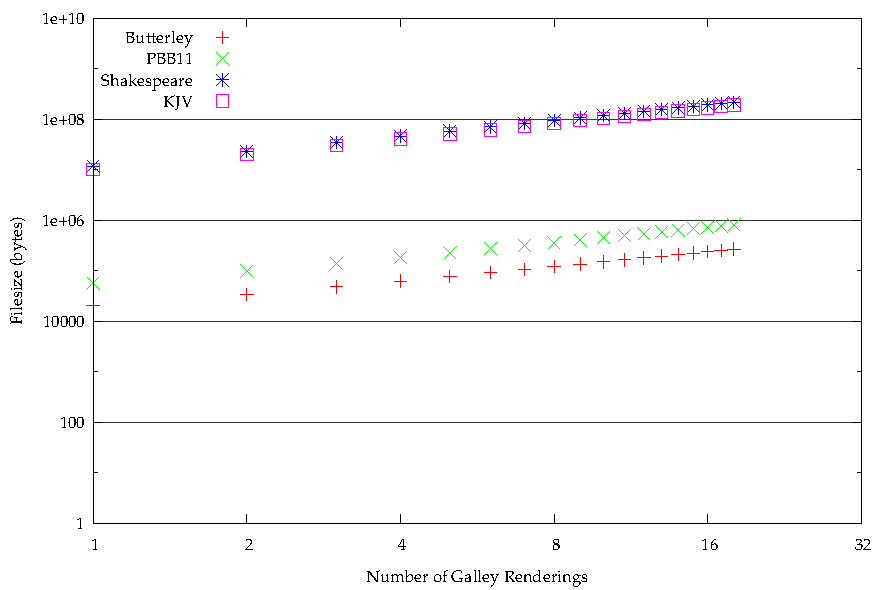
\includegraphics[width=\textwidth]{gnuplot/4-b}
  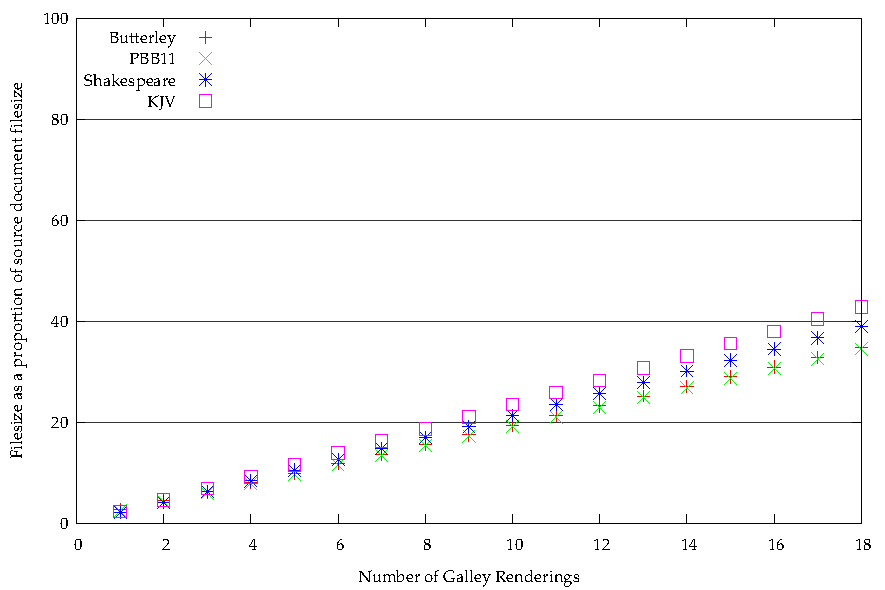
\includegraphics[width=\textwidth]{gnuplot/4-s}
  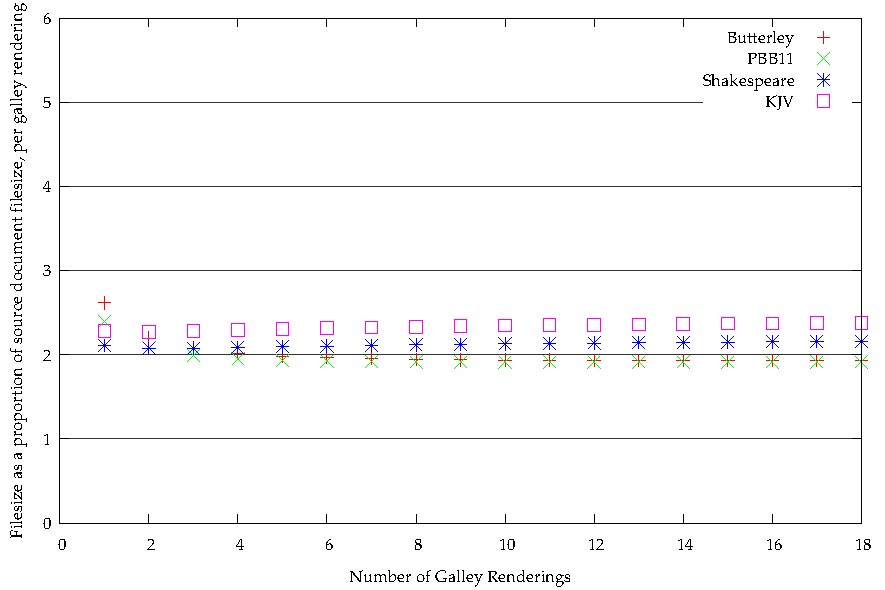
\includegraphics[width=\textwidth]{gnuplot/4-r}
  \end{center}
  \caption[Filesizes with an ordered dictionary]{Filesizes of various documents, encoded using an ordered dictionary.}
  \label{fig:size-ord}
\end{figure}



\begin{figure}
  \begin{center}
  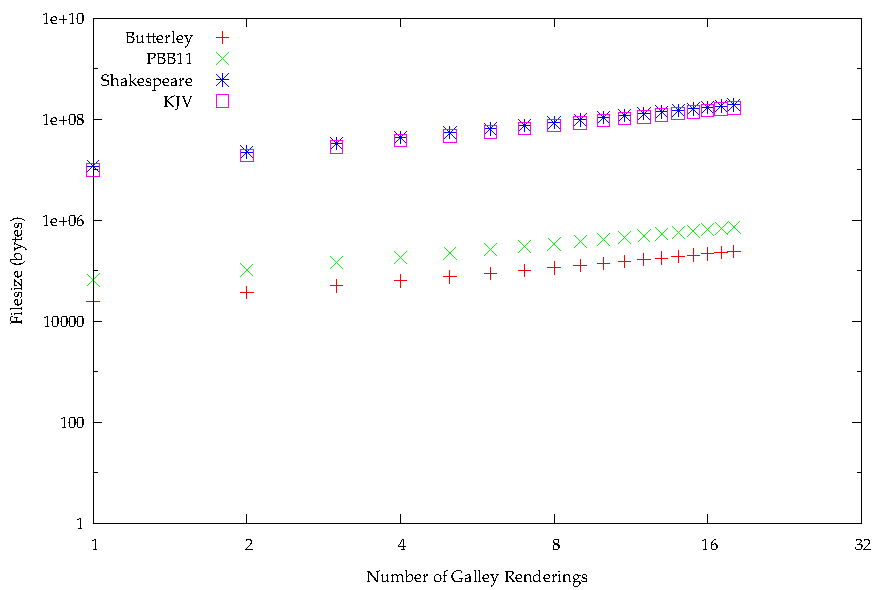
\includegraphics[width=\textwidth]{gnuplot/5-b}
  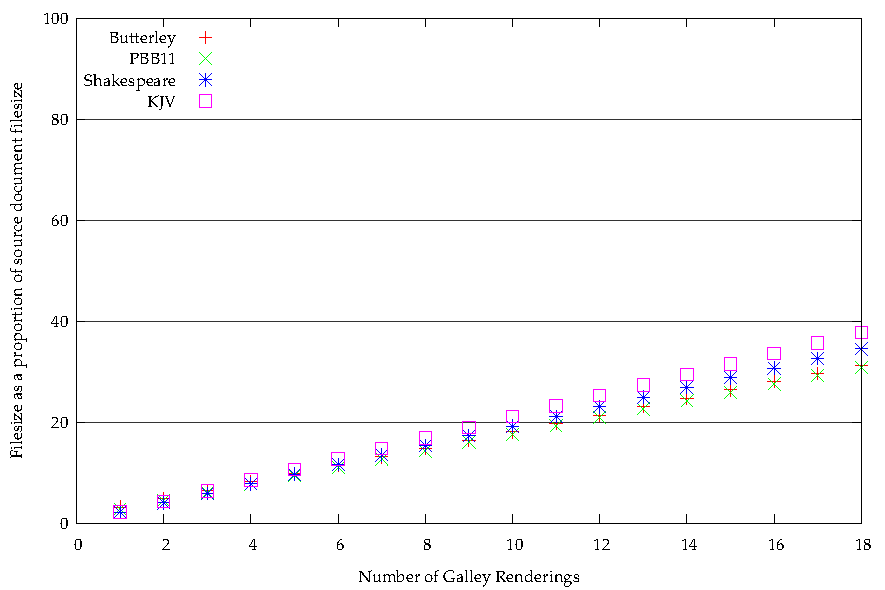
\includegraphics[width=\textwidth]{gnuplot/5-s}
  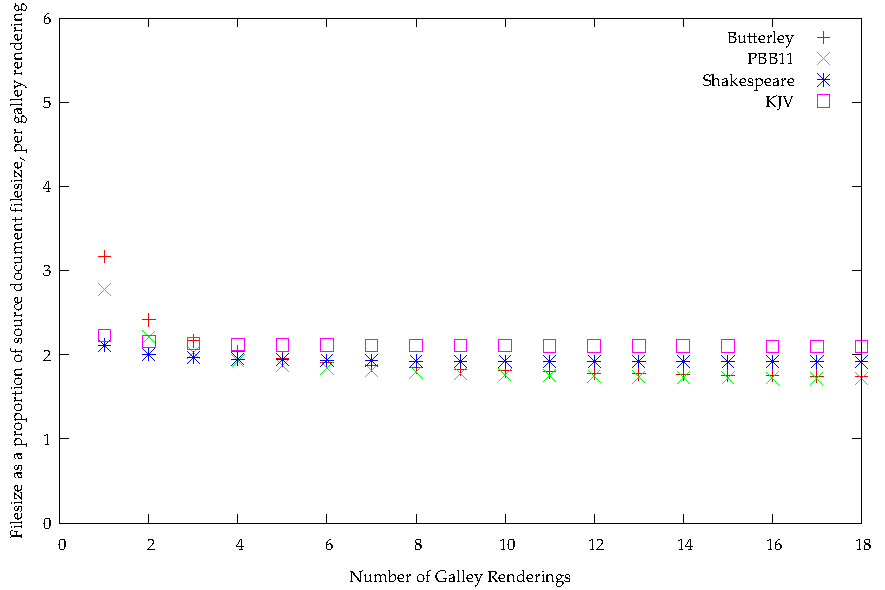
\includegraphics[width=\textwidth]{gnuplot/5-r}
  \end{center}
  \caption[Filesizes with relative positioning]{Filesizes of various documents, encoded using an ordered dictionary with word widths, and position deltas in the Galley Structure Tree.}
  \label{fig:size-deltas}
\end{figure}



\begin{sidewaysfigure}
  \begin{center}
  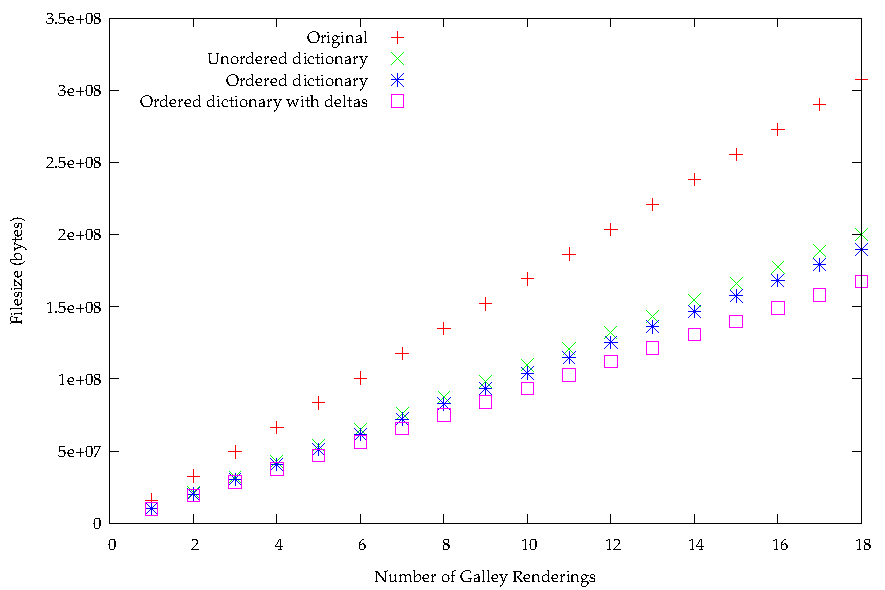
\includegraphics[height=0.5\textheight]{gnuplot/kjv-b}
  \end{center}
  \caption[Comparison of filesizes from all encodings]{A comparison of filesizes produced by all encodings, using the King James Version of the Bible as a sample document.}
  \label{fig:size-all-b}
\end{sidewaysfigure}

\begin{sidewaysfigure}
  \begin{center}
  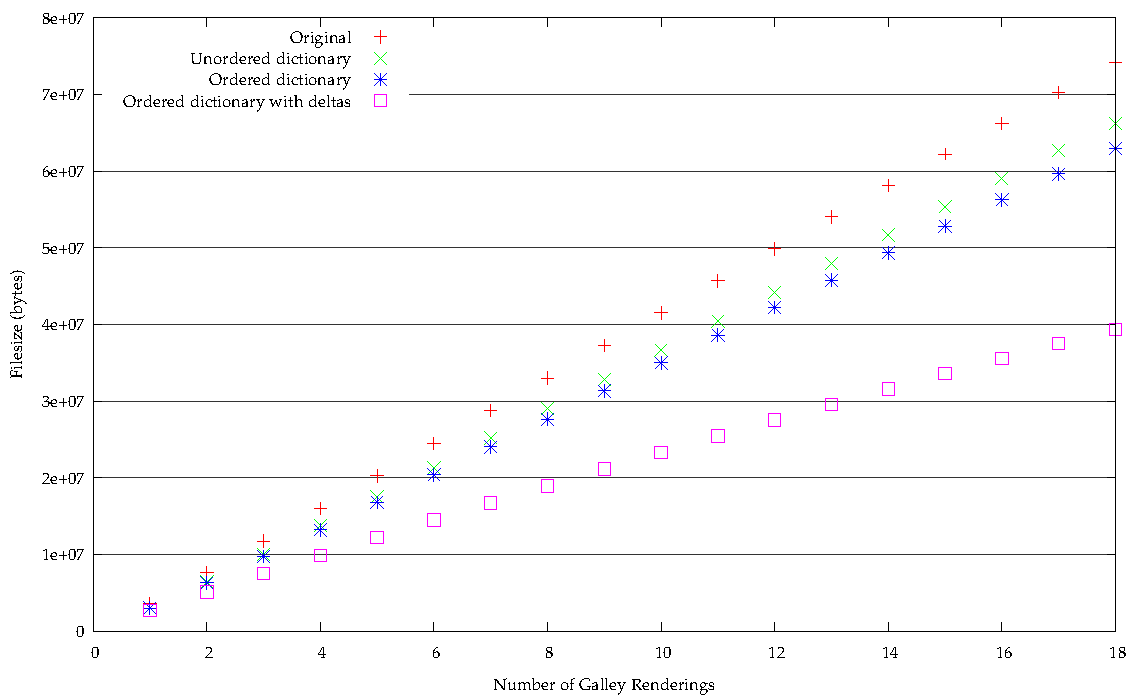
\includegraphics[height=0.5\textheight]{gnuplot/kjv-gz}
  \end{center}
  \caption[Comparison of gzips of all encodings]{A comparison of filesizes of all encodings after gzipping, using the King James Version of the Bible as a sample document. Note the substantial improvement in compression of the encoding that uses position deltas, over the variants that use absolute positioning.}
  \label{fig:size-all-gz}
\end{sidewaysfigure}


% \begin{table}
%     \myfloatalign
%   \begin{tabularx}{\textwidth}{lXXXXXX} %\toprule
%     & \multicolumn{2}{l}{\textsc{source text}} & \multicolumn{2}{l}{\textsc{orig. scheme}} & \multicolumn{2}{l}{\textsc{dictionary}} \\
%     & \textsc{plain} & \textsc{gz} & \textsc{plain} & \textsc{gz} & \textsc{plain} & \textsc{gz} \\ \midrule
%     PBB11~\cite{Pinkney2011} & 23\textsc{k} & 9.4\textsc{k} & 627\textsc{k} & 145\textsc{k} & 314\textsc{k} & 111\textsc{k} \\ \midrule
%     King James Bible & 4.3\textsc{m} & 1.4\textsc{m} & 144\textsc{m} & 32\textsc{m} & 73\textsc{m} & 24\textsc{m} \\ 
%     \bottomrule
%   \end{tabularx}
%   \caption[Comparison of filesizes]{Comparison of filesizes using various encoding methods}  \label{tab:filesize}
% \end{table}


\clearpage


\subsection{Discussion}

It is fairly clear from the preceding graphs that so long as some thought is put in, a lot of redundancy can be squeezed out of the data, without the need to resort to aggressive compression methods that require significant computation during decompression.

Nevertheless, Figures \ref{fig:size-all-b}~and~\ref{fig:size-all-gz} suggest that a significant amount of redundancy remains in each of the encoding schemes: on gzipping, the filesizes are reduced by some 66--75\%. Some of this can be attributed to \gls{json}'s syntax, but it is likely that the blame lies more with the data itself. The dictionary itself is not particularly compact. No advantage is taken of words that share common substrings, nor of words that have identical widths.
Algorithms that do take advantage of substrings, for example \textsc{lz77},\hspace{0pt}\cite{Ziv1977} tend not to have been designed with fast decompression in mind. It is vital that the complexity of any required decompression does not dominate that of the layout process itself.

A further manner in which the data could be compressed is to take advantage of the fact that the values of the position deltas are often repeated, particularly when lines have even spacing between words, which is in the vast majority of cases. This can be seen fairly clearly in Listing~\ref{lst:deltasdata} on page~\pageref{lst:deltasdata}. A second ``dictionary'' can be created in which to store these position deltas. Informal experimentation has suggested this would reduce filesizes by a further 10--15\%, and gzipped filesizes by a further 5\%.

\section{Summary}

The result of the work in this chapter is a reasonably compact version of the document representation model developed in Chapter~\ref{ch:floats}. As an example, a 7-galley malleable version of the King James Bible in the original representation was around 150~\textsc{mb}, and in the most compact representation around 57~\textsc{mb}. This is still considerably larger than the source document (around 4.3~\textsc{mb} as plain text) but does contain data that allows the content to be typeset to seven different widths. The graphs in Figure~\ref{fig:size-deltas} show that each included rendering contributes approximately twice the size of the original plaintext source.

Since the compression used relies entirely on array lookups, the computational overhead for decompression is kept to a minimum. Dealing with moderately larger file sizes seems a reasonable price to pay.

\part{Analysis}
\chapter{Technical Analysis}\label{ch:techanalysis}


%\section{View-time Operations}

Chapter~\ref{ch:intro} (and in particular Section~\ref{sec:goodtypesetting}) provides an overview of some of the operations required when laying out a document. This chapter goes into a little more detail, and contrasts the operations required to view fixed and flowable documents against the operations required to view malleable documents.

\section{Fixed Document Formats}
Documents in a fixed format are rendered in a manner similar to the following:
{\singlespacing
\begin{lstlisting}
parse and tokenise the document layout instructions;
foreach (layout instruction) {
    interpret and execute the instruction;
}
paint the results to the screen;
\end{lstlisting}
}
Crucially, the layout instructions are declarative, and do not permit computation, which ensures that the document is always rendered identically.~\cite{Bagley2007}

\newpage
\section{Flowable Document Formats}

When a document in a flowable format is to be laid out, the process is as follows:
{\singlespacing
\begin{lstlisting}
parse the source to identify flowable blocks;
foreach (flowable block) {
    apply a line-breaking algorithm;
}
paint the results to the screen;
\end{lstlisting}
}

This process generates information similar to that contained in fixed-format documents, which is then used to drive the painting of contents to the screen.

The line breaking algorithm can be as simple as or complex as desired. In most cases, the line-breaking algorithm used by flowable documents is reasonably simple, and will take a first fit approach. This will be of the form:

{\singlespacing
\begin{lstlisting}
parse block to identify all possible breakpoints;
while (non-breakable items remain to be laid out) {
    place one item on the current line;
    if (there is not space for the next item) {
        adjust spacing between items to justify;
        move to a new line;
    }
}
\end{lstlisting}
}

As is noted in Section~\ref{sec:goodtypesetting}, first-fit algorithms do not generally result in well-typeset output. The simplest of these algorithms will not attempt to identify potential hyphenation points. More complex layout algorithms that search for ``optimal'' layouts usually require a considerable amount of backtracking.

\newpage
\section{Malleable Documents}

The layout algorithm for a malleable document is as follows. First, the penalties are calculated:

{\singlespacing
\begin{lstlisting}
foreach (included galley rendering) {
    compute penalty for the rendering at current page width;
}
select the rendering with the minimum penalty;
\end{lstlisting}
}


Then, using the galley rendering that has the lowest penalty, the content is laid out onto the screen:

{\singlespacing
\begin{lstlisting}
foreach (paragraph-level item in selected galley rendering){
    foreach (line-level item in paragraph) {
        use precomputed data to place words;
    }
}
paint the results to the screen;
\end{lstlisting}
}
Crucially, a number of complex steps have been moved from view-time to compile-time (as they are for fixed-format documents) but without flowability being sacrificed:
\begin{itemize}
 \item The source is already parsed into a form optimised for layout
 \item The line-breaking algorithm has been entirely precomputed
\end{itemize}
One step has been added: each included galley rendering must be examined once before layout, in order to ascertain its ``penalty'' for use. The penalty is based entirely on the width of the page, and the \gls{measure} (width) of the galley rendering.%, and is described in more detail in Section~\ref{sec:layout}.

This penalty is calculated by taking the extra required horizontal whitespace (which can be envisaged as slack between columns) and weighting this to further penalise large numbers of columns. This weighting is achieved by multiplying by a smaller-than-linear function of the number of columns, such as a square root or logarithm.

Many low-power processors do not come with floating-point hardware as standard (for example the \textsc{arm} range of processors) which might suggest that these are poor choices of functions since they must be emulated using integer and bitwise operations only. This is not particularly important, for a number of reasons. Firstly, it has been shown previously~\cite{Lomont2003} that it is often possible to use mathematical analysis to find extremely good approximations for such functions. Secondly, the range of inputs to such a function would be limited to integers ranging from 1 to (in an extreme case) about 20, so the values could be pre-computed and stored in a lookup table. Thirdly, the penalty (and hence the root or logarithm) is calculated precisely once for each included galley rendering: in section~\ref{sec:inc-renderings} it is suggested that between three and seven galley renderings should be included in any one document. Given these facts, it is clear that there should be little impact from using such a function in the penalty calculation.

\vspace{2em}

Most importantly, since the line-breaking algorithm has been moved to compile-time, there is no longer any requirement to limit its complexity. In fact, should the need (or desire) arise, the text layout can be hand-tuned, or \emph{entirely hand-typeset}, with no consequences at view-time.


\section{Handling of Floats}

The grid-based layout system devised in Section~\ref{sec:gridlayout} works in a similar manner to a first-fit line-breaking algorithm, in that it places elements on the page in order, in the first place they will fit. In the case of this system, each element is a floatable figure or line of text. Elements that are the same size as a single grid cell, such as lines of text set in the main point size, can simply be placed in the first empty slot in the current column, or the first empty slot in the next column, should there be no empty spaces.  For the placement of elements that are larger than a single grid cell, there is some overhead required to step through the grid until a suitable position can be found. Once a position has been found, each grid cell that it overlaps must be marked as being reserved.

In the worst case, this algorithm does have a greater-than-linear time complexity. In practice, so long as the number of floats does not become excessive (which would cause the grid to be walked many times to search for suitably large gaps) the algorithm runs in linear time.

The placement of floats is subject to certain constraints: they must span integer multiples of columns, and can only be placed aligned to grid cells. This is very different to the model used for floats in \gls{html}, whereby floats may be positioned arbitrarily, and text flowed around them. Although a little more restrictive than \gls{html}, this system is capable of producing layouts that lend themselves to many types of document that are likely to be read on \ebook{} readers. The next chapter discusses this in more detail.


\chapter{Aesthetic Analysis}\label{ch:aesthetics}

\section{Placement of Floats}
Since all text layout is precomputed, the only remaining concern is that the columns of text and floats are laid out in a pleasing manner. Plass~\cite{Plass1981} devised a system to perform optimal placement of floats within text, whereby float placement is penalised by the square of the distance from its intended position. He showed this to be NP-hard, though also showed a similar (but less ``optimal'') system that uses linear penalties can be made to be computationally tractable.

Br\"uggemann-Klein et al.~\cite{Bruggemann-Klein1995} suggest that Plass's method is only optimal for a given value of ``optimal''. They proposed that a superior metric for float placement is to minimise the number of page turns that a reader must perform when reading the document from front to back. This is a desirable characteristic for a pagination algorithm that runs on an \ebook{} reader, because page turns tend to be slow, particularly on devices with electronic paper displays. Unfortunately, the algorithm used runs in quadratic time, and which limits its usefulness to this system.

In essence, the assumption that Plass's float placement algorithm produces the most optimal layouts may be slightly short-sighted: \emph{other pagination schemes are available!} Clearly, using a computationally intractable algorithm such as Plass's is likely to have significant impact on the demand for computation at view-time. As with many facets of the system described in this thesis, the float placement algorithm was chosen with efficiency in mind.

The float placement algorithm that has been developed for use with the malleable document system also attempts to minimise the distance between the actual and intended positioning of floats: if a float can be placed directly at its intended position, then it will be, otherwise it will be placed in the next available space. (Figure~\ref{fig:gridlayout} on page~\pageref{fig:gridlayout} demonstrates this process.)

Whilst this algorithm does not perform any lookahead or backtracking in order to place floats optimally, experiments have shown that in most cases, floats are placed directly in their intended positions or at the top of adjacent columns, and are only occasionally moved across page boundaries. Figures \ref{fig:example-portrait}, \ref{fig:example-landscape}, and~\ref{fig:example-ereader} show some examples of layouts produced using this algorithm.

As it stands, the algorithm does not avoid widowed or orphaned lines, or single lines directly before or after floats. This can be seen clearly in Figure~\ref{fig:example-ereader} at the top of the fourth page, where the float has spanned both columns and taken up all the space on the page, with the exception of one line at the top of each column. It would not be too difficult to add a constraint that states that single lines of text at the top or bottom of the page should never be allowed, which could be enforced by leaving extra lines blank, pushing the text forward, though it is possible that this may harm the balance of the page if it causes columns to have uneven lengths.

\begin{figure}
\begin{center}
\fbox{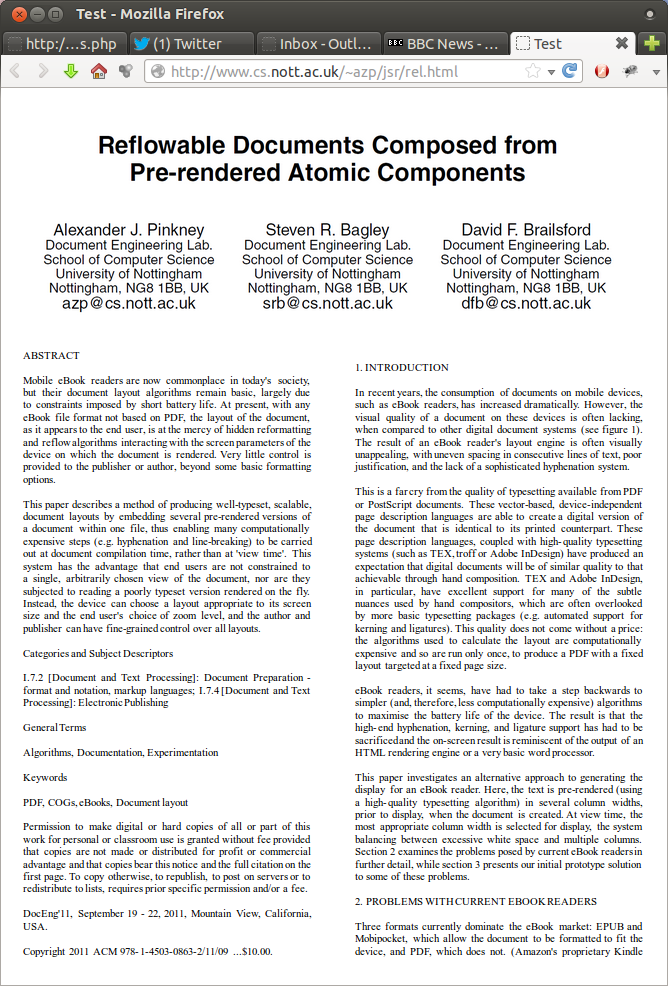
\includegraphics[trim=0in 0in 0in 1.2in, clip=true, width=0.47\textwidth]{gfx/p1}}\hspace{0.01\textwidth}
\fbox{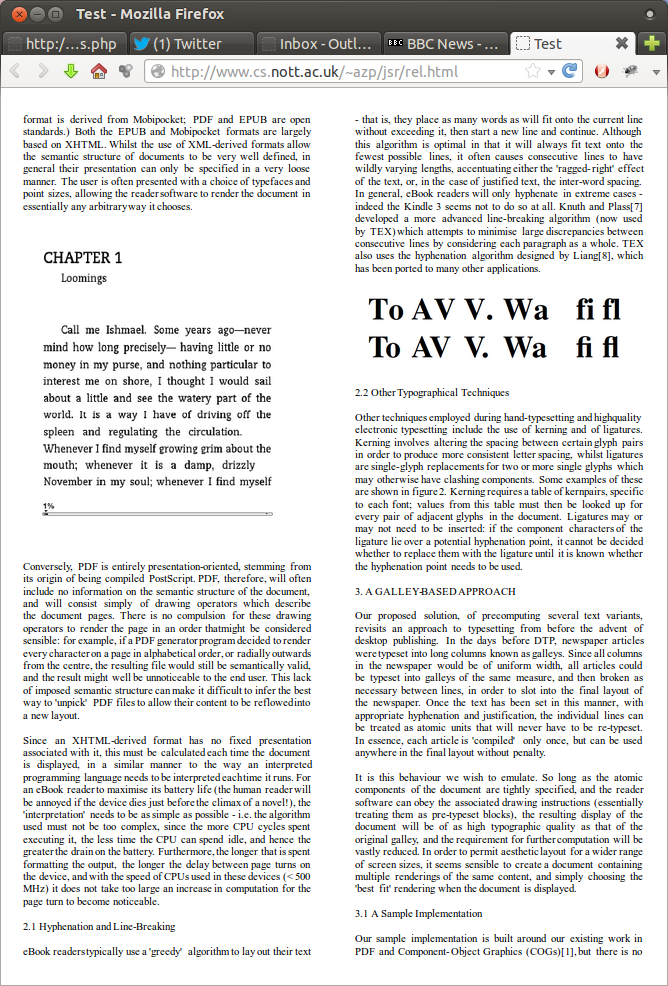
\includegraphics[trim=0in 0in 0in 1.2in, clip=true, width=0.47\textwidth]{gfx/p2}}

\vspace{0.2in}
\fbox{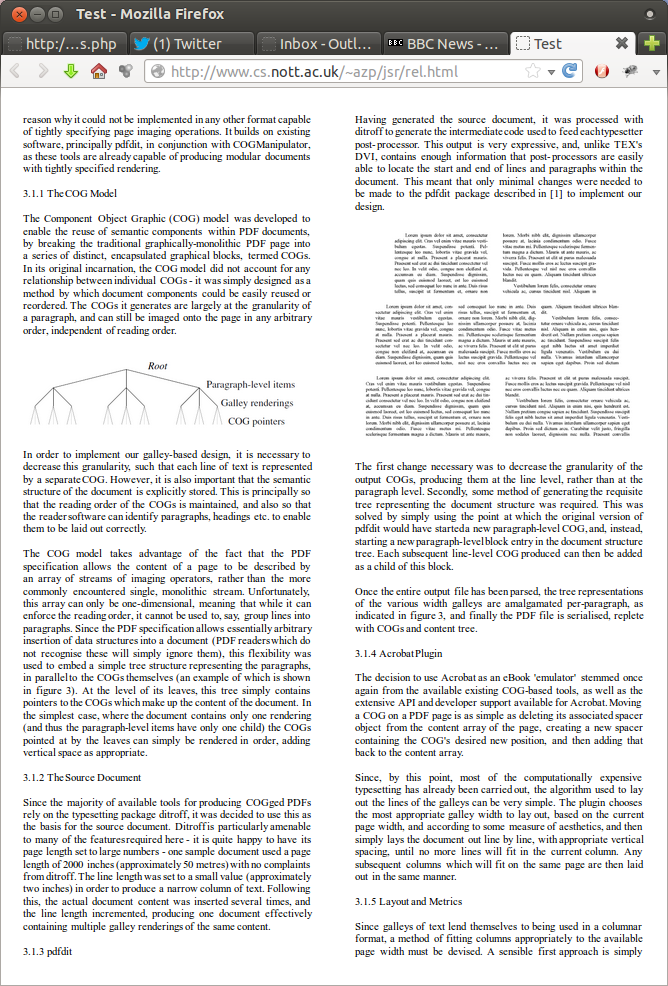
\includegraphics[trim=0in 0in 0in 1.2in, clip=true, width=0.47\textwidth]{gfx/p3}}\hspace{0.01\textwidth}
\fbox{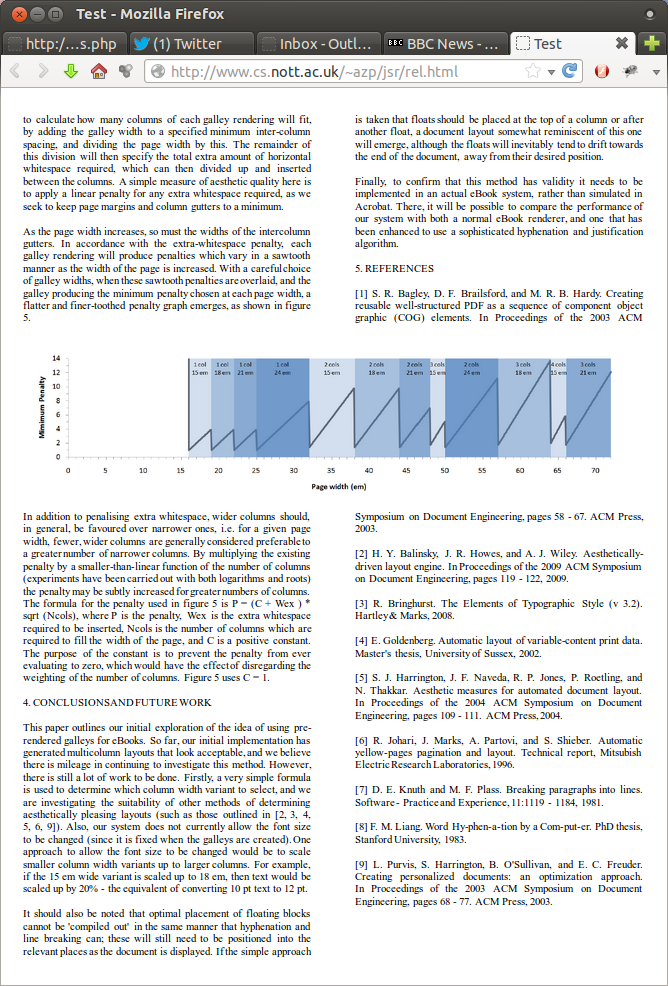
\includegraphics[trim=0in 0in 0in 1.2in, clip=true, width=0.47\textwidth]{gfx/p4}}
\end{center}
\caption[A sample of document layout]{\cite{Pinkney2011} laid out by the malleable document system, running in Mozilla Firefox. The page size has been selected to resemble that of A4 paper in a portrait orientation.}
\label{fig:example-portrait}
\end{figure}

\begin{sidewaysfigure}
\begin{center}
\fbox{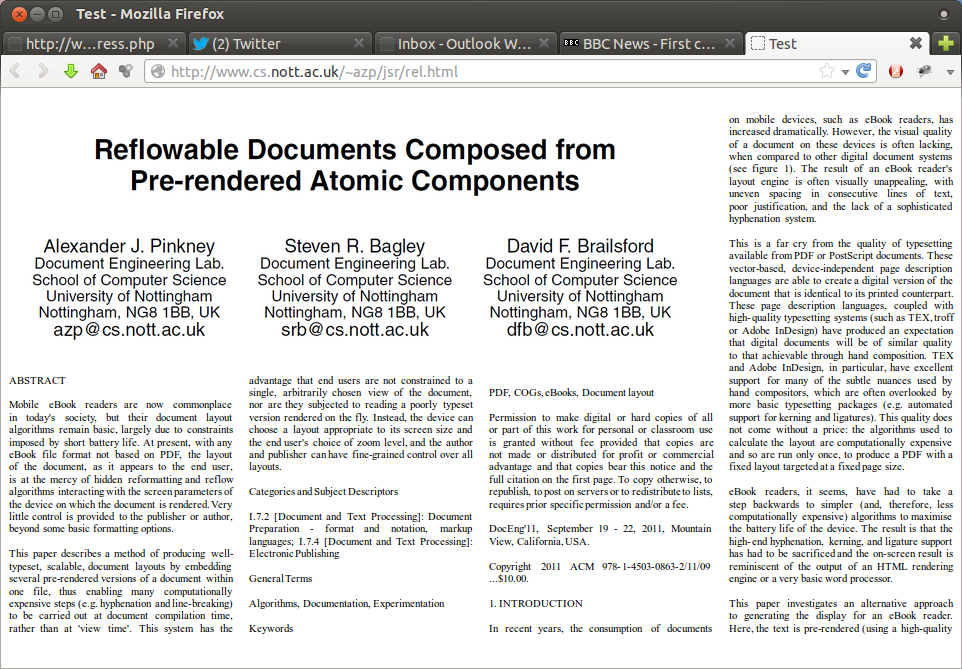
\includegraphics[trim=0in 0in 0in 1.2in, clip=true, width=0.45\textwidth]{gfx/q1}}\hspace{0.05\textwidth}
\fbox{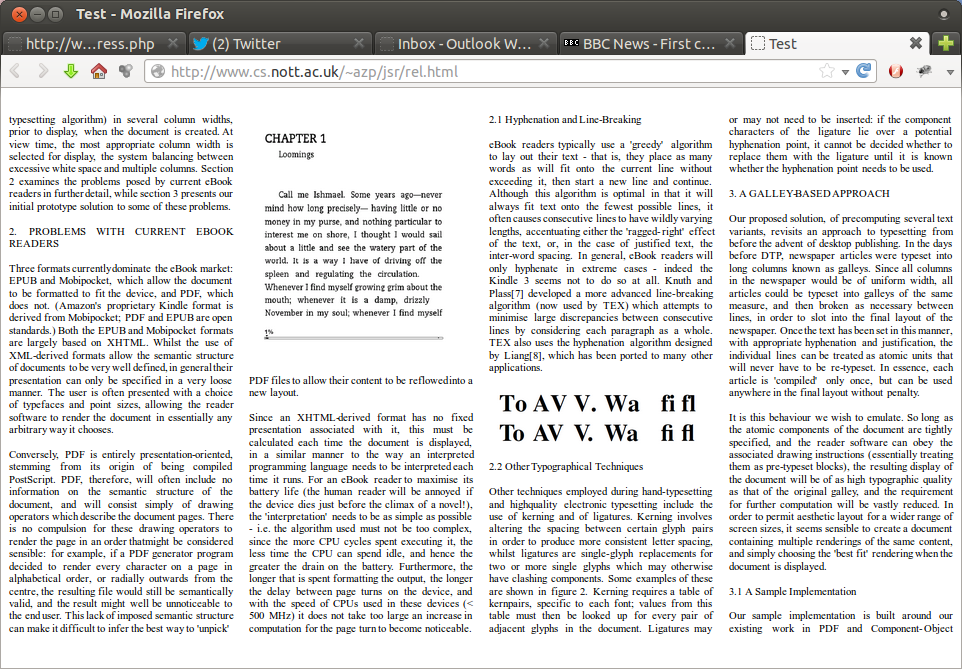
\includegraphics[trim=0in 0in 0in 1.2in, clip=true, width=0.45\textwidth]{gfx/q2}}

\vspace{0.2in}
\fbox{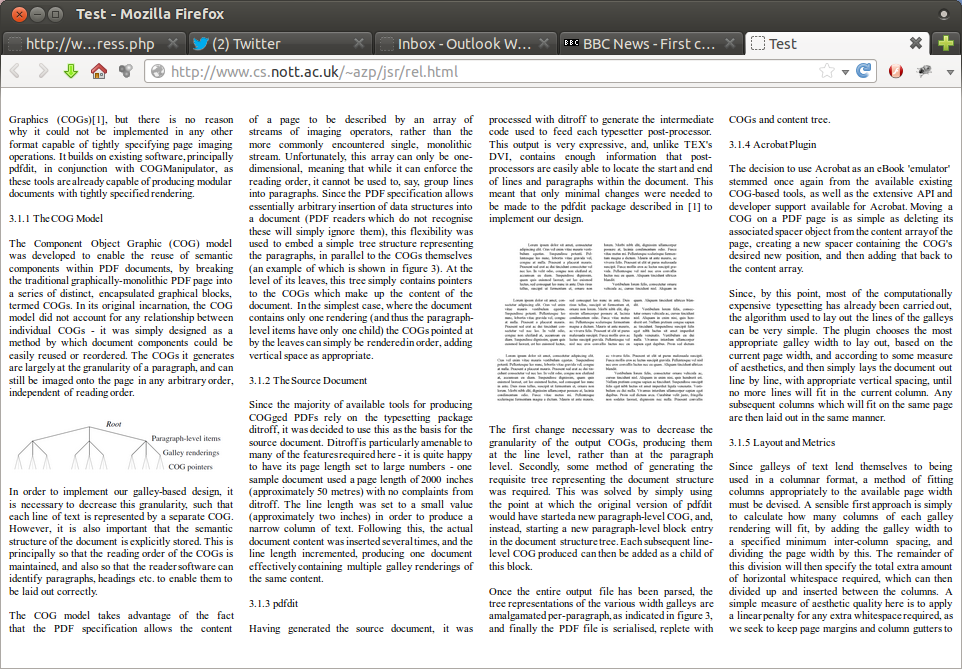
\includegraphics[trim=0in 0in 0in 1.2in, clip=true, width=0.45\textwidth]{gfx/q3}}\hspace{0.05\textwidth}
\fbox{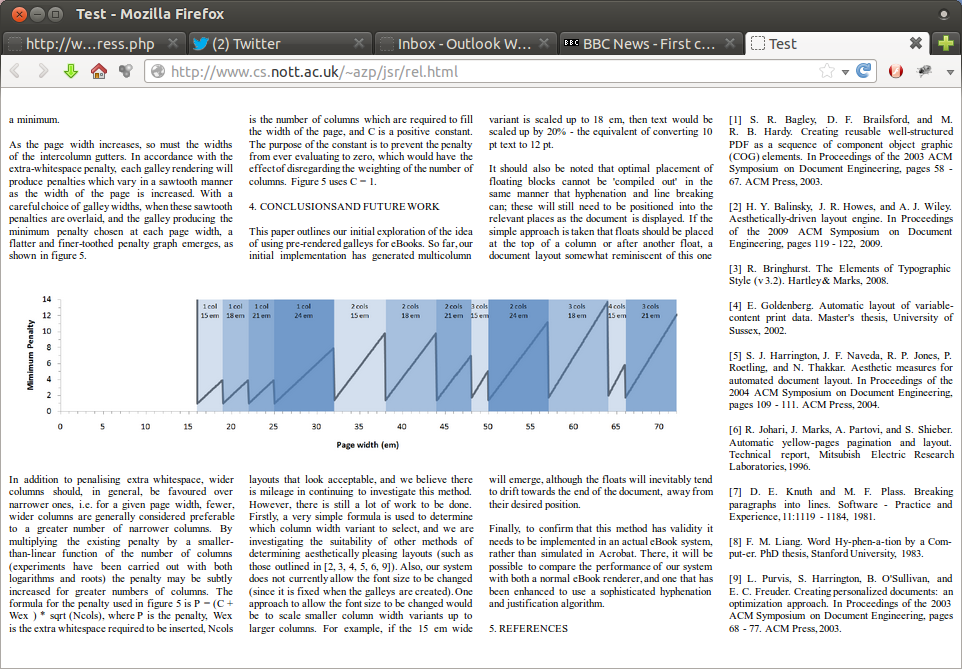
\includegraphics[trim=0in 0in 0in 1.2in, clip=true, width=0.45\textwidth]{gfx/q4}}
\end{center}
\caption[A sample of document layout]{\cite{Pinkney2011} laid out by the malleable document system, running in Mozilla Firefox. The page size has been selected to resemble that of A4 paper in a landscape orientation.}
\label{fig:example-landscape}
\end{sidewaysfigure}

\begin{figure}
\begin{center}
\newlength{\imgwid} \setlength{\imgwid}{0.29\textwidth}
\fbox{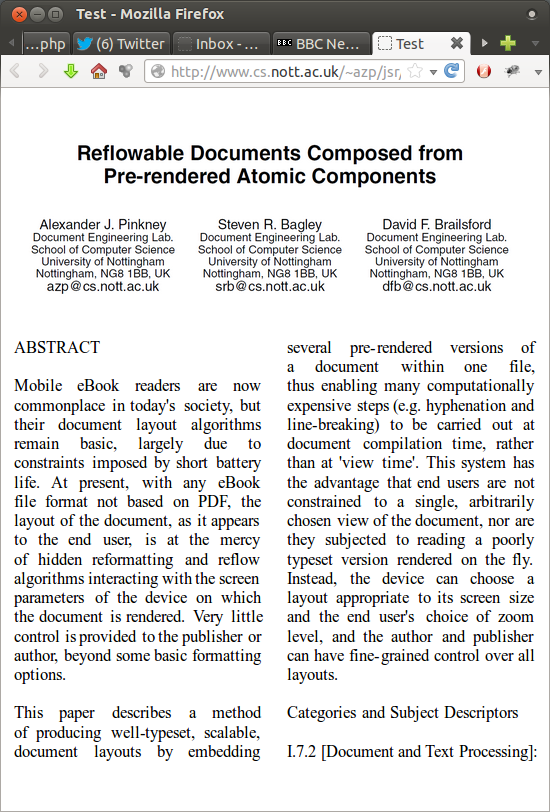
\includegraphics[trim=0in 0in 0in 1.2in, clip=true, width=\imgwid]{gfx/r1}}
\fbox{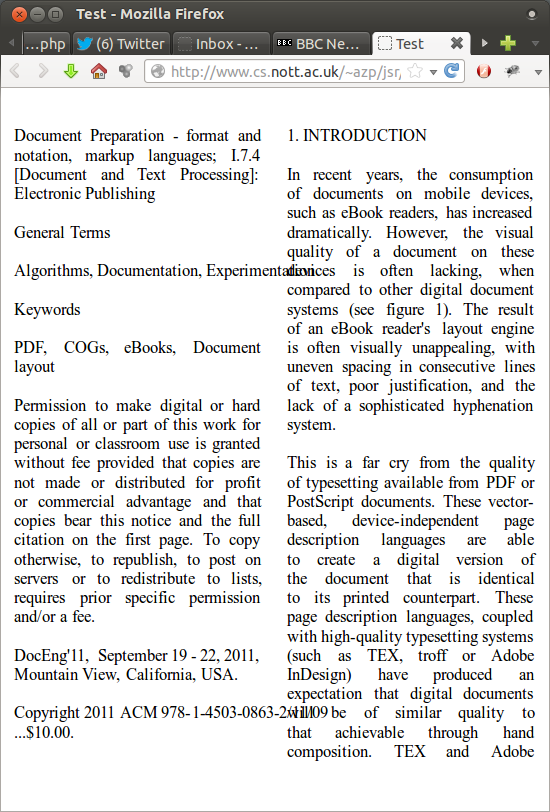
\includegraphics[trim=0in 0in 0in 1.2in, clip=true, width=\imgwid]{gfx/r2}}
\fbox{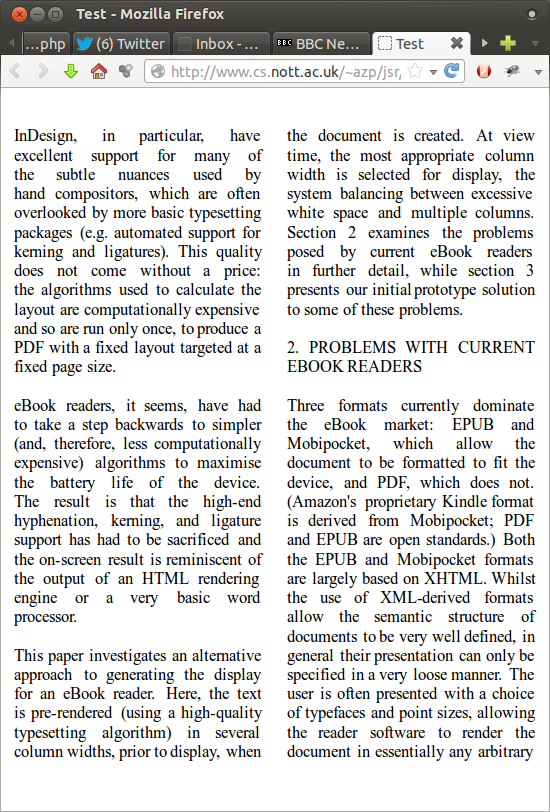
\includegraphics[trim=0in 0in 0in 1.2in, clip=true, width=\imgwid]{gfx/r3}}
\fbox{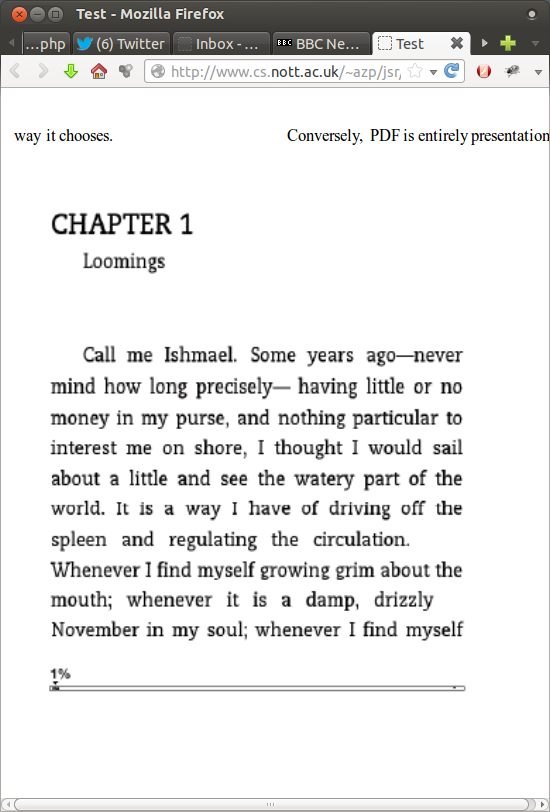
\includegraphics[trim=0in 0in 0in 1.2in, clip=true, width=\imgwid]{gfx/r4}}
\fbox{\includegraphics[trim=0in 0in 0in 1.2in, clip=true, width=\imgwid]{gfx/r5}}
\fbox{\includegraphics[trim=0in 0in 0in 1.2in, clip=true, width=\imgwid]{gfx/r6}}
\fbox{\includegraphics[trim=0in 0in 0in 1.2in, clip=true, width=\imgwid]{gfx/r7}}
\fbox{\includegraphics[trim=0in 0in 0in 1.2in, clip=true, width=\imgwid]{gfx/r8}}
\fbox{\includegraphics[trim=0in 0in 0in 1.2in, clip=true, width=\imgwid]{gfx/r9}}
\fbox{\includegraphics[trim=0in 0in 0in 1.2in, clip=true, width=\imgwid]{gfx/r10}}
\fbox{\includegraphics[trim=0in 0in 0in 1.2in, clip=true, width=\imgwid]{gfx/r11}}
\fbox{\includegraphics[trim=0in 0in 0in 1.2in, clip=true, width=\imgwid]{gfx/r12}}
\fbox{\includegraphics[trim=0in 0in 0in 1.2in, clip=true, width=\imgwid]{gfx/r13}}
\fbox{\includegraphics[trim=0in 0in 0in 1.2in, clip=true, width=\imgwid]{gfx/r14}}
\end{center}
\caption[A sample of document layout]{\cite{Pinkney2011} laid out by the malleable document system, running in Mozilla Firefox. The page size has been selected to resemble that of an \ebook{} reader in a portrait orientation.}
\label{fig:example-ereader}
\end{figure}

\section{Measures of Aesthetic Quality}
In their 2004 paper, Harrington et al.~\cite{Harrington2004} identified nine aesthetic measures for automated document layout. A number of these measures (alignment, regularity, uniform separation, white-space free-flow, uniformity) are inherently well satisfied by this system, due to its use of a grid to provide regular layout. 


\section{The Importance of Typography}
Many studies\cite{Hill1999,Bringhurst2008,Voorhees2011,Legge2011} have shown that good typography is the key to readability. In particular, it is stated in \emph{The Magic of Reading}~\cite{Hill1999} that both regularity of whitespace between words and the evenness of line lengths are of importance\ed the only way to achieve this is to use a line-breaking algorithm that attempts to make line lengths as even as possible. Since line-breaking is performed at compile time, it can be ensured that this is optimal when the malleable document is created. Figure~\ref{fig:greek} compares an ``optimal'' algorithm (Knuth-Plass~\cite{Knuth1981}) against the default layout of a web browser (a first fit, greedy approach).

\begin{figure}
\begin{center}
\includegraphics[height=0.8\textheight]{gfx/greek}
\end{center}
\caption[Knuth-Plass layout versus a first-fit algorithm]{Knuth-Plass layout (left) versus a first-fit algorithm (right). Note that Knuth-Plass results in looser spacing of certain lines where it helps avoid extremely loosely-set lines ahead. Even without using hyphenation (this implementation of Knuth-Plass does not include a hyphenation algorithm) the results are noticeable. }
\label{fig:greek}
\end{figure}

%   - Greeking\\
%       - Default browser layout vs mine\\
%       - Look at \cite{Harrington2004} for some measures and say why mine is awesome\\
%   - some discussion of choices of galley widths for best performance


\section{Summary}
The malleable document system devised in this thesis was designed to be used for linear documents whose content is primarily text. Examples of such documents would be novels and scientific papers, but not reference books or graphic-heavy documents such as comics or children's picture books.

The layouts produced by this system are visually very similar to those of both newspapers and scientific papers, and can be flowed to fit virtually any page size. For smaller screen sizes, where single- or double-column spreads occur, the layouts closely resemble those of physical books and magazines.

\todo{Sum up a bit better}

\chapter{Conclusions, Evaluation, and Future Work}\label{ch:conclusions}


The system described in chapter~\ref{ch:floats} has only very basic support for floats. A particular limitation is that unlike paragraphs, each float has only one rendering, which must be scaled up or down as required, to fit across multiples of columns. Whilst for image-based figures or illustrations, this is probably already the desired behaviour, other types of floats, such as tables or code listings, would almost certainly benefit from the inclusion of multiple width renderings, with the choice of which rendering to display to be made at view-time. % Say that these could be differing hand-renderings, or automated from some source? Probably don't need to...

% coordinating breakpoints? might leave this until I have something sensible to say

Since the malleable document and viewer are composed entirely from HTML, CSS, and JavaScript\ed the core technologies behind EPUB\,---\,modifying the system to produce self-contained EPUB files seems an obvious next step.

%%%%%%%%%%%%%%%%%%%%%%%%%%%%%%%%%%%%%%%%%%%%%%%%%%
\singlespacing

% ********************************************************************
% Backmatter
%*******************************************************
\appendix
\cleardoublepage
\part{Appendices}

%********************************************************************
% Appendix
%*******************************************************
% If problems with the headers: get headings in appendix etc. right
\markboth{\spacedlowsmallcaps{Appendices}}{\spacedlowsmallcaps{Appendices}}
%\chapter{Source Code Listings}

% TODO: Render source code with some other tool and include as a figure. This is breaking LaTeX.

%\section{Paragraph Splitter}
%\label{app:parsplitter}
%\subsection{ParSplitter.java}
%\lstinputlisting[nolol,language=Java,tabsize=4,stringstyle=\color{blue},basicstyle=\ttfamily\scriptsize]{../JSReflow/ParSplitter/src/ParSplitter.java}

%\newpage

\cleardoublepage
\chapter{A Sample Malleable Document}
\label{app:sampledoc}

The following pages contain the full layout data of a reasonably short ($\sim$1200 word) document: the Wikipedia entry for The Butterley Company. (See \url{http://en.wikipedia.org/wiki/Butterley_Company}).

It contains three galley renderings, and has ordered dictionaries both for words, and for position deltas.

\newpage
\includepdf[pages=-,scale=.8,pagecommand={}]{butterley.pdf}



\cleardoublepage
\chapter{Sample Layouts}
\label{app:layouts}

All the layouts in this section are of the author's 2011 paper, \emph{Reflowable Documents Composed from Prerendered Atomic Components}.\cite{Pinkney2011}

All the Malleable Document System layouts use the same selection of galley renderings as were used in Rendering D of the user study\ed see Table~\ref{tab:galleypool} on page~\pageref{tab:galleypool}.


\newpage

\section{Layout by the Malleable Document System}

\newlength{\imgwid}

\subsection{Rendered by Mozilla Firefox on a PC}
\label{app:layout-ff}

\cite{Pinkney2011} laid out by the malleable document system, running in Mozilla Firefox on a PC. The page size has been selected to resemble that of A4 paper in a portrait orientation.

\begin{center}
\setlength{\imgwid}{0.47\textwidth}
\fbox{\includegraphics[trim=0in 0in 0in 1.2in, clip=true, width=\imgwid]{gfx/p1}}\hspace{0.01\textwidth}
\fbox{\includegraphics[trim=0in 0in 0in 1.2in, clip=true, width=\imgwid]{gfx/p2}}

\vspace{0.2in}
\fbox{\includegraphics[trim=0in 0in 0in 1.2in, clip=true, width=\imgwid]{gfx/p3}}\hspace{0.01\textwidth}
\fbox{\includegraphics[trim=0in 0in 0in 1.2in, clip=true, width=\imgwid]{gfx/p4}}
\end{center}


\clearpage


\cite{Pinkney2011} laid out by the malleable document system, running in Mozilla Firefox on a PC. The page size has been selected to resemble that of A4 paper in a landscape orientation.

\begin{center}
\setlength{\imgwid}{0.45\textwidth}
\fbox{\includegraphics[trim=0in 0in 0in 1.2in, clip=true, angle=90, width=\imgwid]{gfx/q2}}\hspace{0.05\textwidth}
\fbox{\includegraphics[trim=0in 0in 0in 1.2in, clip=true, angle=90, width=\imgwid]{gfx/q4}}

\vspace{0.2in}
\fbox{\includegraphics[trim=0in 0in 0in 1.2in, clip=true, angle=90, width=\imgwid]{gfx/q1}}\hspace{0.05\textwidth}
\fbox{\includegraphics[trim=0in 0in 0in 1.2in, clip=true, angle=90, width=\imgwid]{gfx/q3}}
\end{center}


\clearpage


\cite{Pinkney2011} laid out by the malleable document system, running in Mozilla Firefox on a PC. The page size has been selected to resemble that of an \ebook{} reader in a portrait orientation.

\label{app:p:layout-ff-ereader}
\begin{center}
\setlength{\imgwid}{0.26\textwidth}
\fbox{\includegraphics[trim=0in 0in 0in 1.2in, clip=true, width=\imgwid]{gfx/r1}}
\fbox{\includegraphics[trim=0in 0in 0in 1.2in, clip=true, width=\imgwid]{gfx/r2}}
\fbox{\includegraphics[trim=0in 0in 0in 1.2in, clip=true, width=\imgwid]{gfx/r3}}
\fbox{\includegraphics[trim=0in 0in 0in 1.2in, clip=true, width=\imgwid]{gfx/r4}}
\fbox{\includegraphics[trim=0in 0in 0in 1.2in, clip=true, width=\imgwid]{gfx/r5}}
\fbox{\includegraphics[trim=0in 0in 0in 1.2in, clip=true, width=\imgwid]{gfx/r6}}
\fbox{\includegraphics[trim=0in 0in 0in 1.2in, clip=true, width=\imgwid]{gfx/r7}}
\fbox{\includegraphics[trim=0in 0in 0in 1.2in, clip=true, width=\imgwid]{gfx/r8}}
\fbox{\includegraphics[trim=0in 0in 0in 1.2in, clip=true, width=\imgwid]{gfx/r9}}
\fbox{\includegraphics[trim=0in 0in 0in 1.2in, clip=true, width=\imgwid]{gfx/r10}}
\fbox{\includegraphics[trim=0in 0in 0in 1.2in, clip=true, width=\imgwid]{gfx/r11}}
\fbox{\includegraphics[trim=0in 0in 0in 1.2in, clip=true, width=\imgwid]{gfx/r12}}
\fbox{\includegraphics[trim=0in 0in 0in 1.2in, clip=true, width=\imgwid]{gfx/r13}}
\fbox{\includegraphics[trim=0in 0in 0in 1.2in, clip=true, width=\imgwid]{gfx/r14}}
\end{center}


\clearpage


\subsection{Chrome on an Android Phone}
\label{app:layout-android}


\cite{Pinkney2011} laid out by the malleable document system, running in Chrome on an Android phone. This example shows a point size that is a little on the small side, but is still readable.

\begin{center}
\setlength{\imgwid}{0.3\textwidth}
\fbox{\includegraphics[width=\imgwid]{gfx/n5_1_01}}
\fbox{\includegraphics[width=\imgwid]{gfx/n5_1_02}}
\fbox{\includegraphics[width=\imgwid]{gfx/n5_1_03}}
\fbox{\includegraphics[width=\imgwid]{gfx/n5_1_04}}
\fbox{\includegraphics[width=\imgwid]{gfx/n5_1_05}}
\fbox{\includegraphics[width=\imgwid]{gfx/n5_1_06}}
\fbox{\includegraphics[width=\imgwid]{gfx/n5_1_07}}
\fbox{\includegraphics[width=\imgwid]{gfx/n5_1_08}}
\end{center}
 

\clearpage

\cite{Pinkney2011} laid out by the malleable document system, running in Chrome on an Android phone, in portrait and in landscape. This example uses a point size that is likely to be readable by a greater range of people. For brevity's sake, only the first three pages of each rendering are shown.

\begin{center}
\setlength{\imgwid}{0.3\textwidth}
\fbox{\includegraphics[width=\imgwid]{gfx/n5_p_1}}
\fbox{\includegraphics[width=\imgwid]{gfx/n5_p_2}}
\fbox{\includegraphics[width=\imgwid]{gfx/n5_p_3}}

\vspace{2em}

\fbox{\includegraphics[height=\imgwid]{gfx/n5_l_1}}
\fbox{\includegraphics[height=\imgwid]{gfx/n5_l_2}}
\fbox{\includegraphics[height=\imgwid]{gfx/n5_l_3}}
\end{center}


\clearpage


\subsection{Safari on an iPad}
\label{app:layout-ipad}

\cite{Pinkney2011} rendered in Safari on a iPad in portrait orientation:
\begin{center}
\setlength{\imgwid}{0.47\textwidth}
\fbox{\includegraphics[width=\imgwid]{gfx/ipad-p1}}
\fbox{\includegraphics[width=\imgwid]{gfx/ipad-p2}}

\vspace{0.3em}

\fbox{\includegraphics[width=\imgwid]{gfx/ipad-p3}}
\fbox{\includegraphics[width=\imgwid]{gfx/ipad-p4}}

\end{center}

\clearpage
\cite{Pinkney2011} rendered in Safari on a iPad in landscape orientation:
\begin{center}
\setlength{\imgwid}{0.8\textwidth}
\fbox{\includegraphics[width=\imgwid]{gfx/ipad-l1}}

\vspace{0.3em}

\fbox{\includegraphics[width=\imgwid]{gfx/ipad-l2}}

\vspace{0.3em}

\fbox{\includegraphics[width=\imgwid]{gfx/ipad-l3}}

\end{center}
\clearpage
\section{Other systems}
\label{app:layout-other}

\subsection{\LaTeX}

\cite{Pinkney2011} as rendered by \LaTeX. The layout is very similar to that produced by the malleable document system (see \ref{app:layout-ff}) though \LaTeX{} favours placing floats at the top of columns, rather than directly at their logical position.

\begin{center}
\setlength{\imgwid}{0.47\textwidth}
\fbox{\includegraphics[trim=0.1in 2in 0.1in 1in, clip=true, width=\imgwid]{gfx/pbb11-1}}\hspace{0.01\textwidth}
\fbox{\includegraphics[trim=0.1in 2in 0.1in 1in, clip=true, width=\imgwid]{gfx/pbb11-2}}

\vspace{0.2in}
\fbox{\includegraphics[trim=0.1in 2in 0.1in 1in, clip=true, width=\imgwid]{gfx/pbb11-3}}\hspace{0.01\textwidth}
\fbox{\includegraphics[trim=0.1in 2in 0.1in 1in, clip=true, width=\imgwid]{gfx/pbb11-4}}
\end{center}



\clearpage



\subsection{\textsc{html}}

\gls{html} version of \cite{Pinkney2011}, as rendered by Mozilla Firefox, scaled to fit multiple screen sizes. Though \gls{html} can stretch to any screen size, it tends to produce typographically inferior results, for example lines that are too long, or line breaking that results in extremely uneven spacing between adjacent lines.

\begin{center}
\setlength{\imgwid}{0.45\textwidth}
\fbox{\includegraphics[trim=0in 0in 0in 1.2in, clip=true, width=\imgwid]{gfx/html1}}\hspace{0.01\textwidth}
\fbox{\includegraphics[trim=0in 0in 0in 1.2in, clip=true, width=\imgwid]{gfx/html2}}

\vspace{0.2in}
\fbox{\includegraphics[trim=0in 0in 0in 1.2in, clip=true, width=\imgwid]{gfx/html3}}\hspace{0.01\textwidth}
\fbox{\includegraphics[trim=0in 0in 0in 1.2in, clip=true, width=\imgwid]{gfx/html4}}
\end{center}



%********************************************************************
% Other Stuff in the Back
%*******************************************************
\printglossaries
\newpage
\doublespacing
%********************************************************************
% Bibliography
%*******************************************************
% work-around to have small caps also here in the headline
\manualmark
\markboth{\spacedlowsmallcaps{\bibname}}{\spacedlowsmallcaps{\bibname}} % work-around to have small caps also
%\phantomsection 
\refstepcounter{dummy}
\addtocontents{toc}{\protect\vspace{\beforebibskip}} % to have the bib a bit from the rest in the toc
\addcontentsline{toc}{chapter}{\tocEntry{\bibname}}
\bibliographystyle{plainnat}
\label{app:bibliography} 
\bibliography{refs}
\singlespacing
\cleardoublepage
\pagestyle{empty}

\hfill

\vfill


\pdfbookmark[0]{Colophon}{colophon}
\section*{Colophon}
This document was typeset using the typographical look-and-feel \texttt{classicthesis} developed by Andr\'e Miede. 
The style was inspired by Robert Bringhurst's seminal book on typography ``\emph{The Elements of Typographic Style}''. \cite{Bringhurst2008}
\texttt{classicthesis} is available for both \LaTeX\ and \mLyX: 
\begin{center}
\url{http://code.google.com/p/classicthesis/}
\end{center}
Happy users of \texttt{classicthesis} usually send a real postcard to the author, a collection of postcards received so far is featured here: 
\begin{center}
\url{http://postcards.miede.de/}
\end{center}
 
\bigskip

\noindent\finalVersionString






%%*******************************************************
% Declaration
%*******************************************************
\refstepcounter{dummy}
\pdfbookmark[0]{Declaration}{declaration}
\chapter*{Declaration}
\thispagestyle{empty}
Put your declaration here.
\bigskip
 
\noindent\textit{\myLocation, \myTime}

\smallskip

\begin{flushright}
    \begin{tabular}{m{5cm}}
        \\ \hline
        \centering\myName \\
    \end{tabular}
\end{flushright}

% ********************************************************************
% Game Over: Restore, Restart, or Quit?
%*******************************************************
\end{document}
% ********************************************************************


% **************************************************************************************************************
% A Classic Thesis Style
% An Homage to The Elements of Typographic Style
%
% Copyright (C) 2011 Andr\'e Miede http://www.miede.de
%
% If you like the style then I would appreciate a postcard. My address 
% can be found in the file ClassicThesis.pdf. A collection of the 
% postcards I received so far is available online at 
% http://postcards.miede.de
%
% License:
% This program is free software; you can redistribute it and/or modify
% it under the terms of the GNU General Public License as published by
% the Free Software Foundation; either version 2 of the License, or
% (at your option) any later version.
%
% This program is distributed in the hope that it will be useful,
% but WITHOUT ANY WARRANTY; without even the implied warranty of
% MERCHANTABILITY or FITNESS FOR A PARTICULAR PURPOSE.  See the
% GNU General Public License for more details.
%
% You should have received a copy of the GNU General Public License
% along with this program; see the file COPYING.  If not, write to
% the Free Software Foundation, Inc., 59 Temple Place - Suite 330,
% Boston, MA 02111-1307, USA.
%
% **************************************************************************************************************
% Note:
%    * You must not use "u etc. in strings/commands that will be spaced out (use \"u or real umlauts instead)
%    * New enumeration (small caps): \begin{aenumerate} \end{aenumerate}
%    * For margin notes: \marginpar or \graffito{}
%    * Do not use bold fonts in this style, it is designed around them
%    * Use tables as in the examples
%    * See classicthesis-preamble.sty for useful commands
% **************************************************************************************************************
% To Do:
%		 * [high] Check this out: http://www.golatex.de/koma-script-warnung-in-verbindung-mit-listings-package-t2058.html
%    * [medium] mathbb in section-titles/chapter-titles => disappears somehow in headlines!!!
% **************************************************************************************************************